\documentclass[a4paper,12pt]{report}

% Importazione pacchetti
\usepackage[utf8]{inputenc}
\usepackage{geometry}
\usepackage{tikz} 
\usetikzlibrary{positioning}
\usepackage{setspace} %gestione degli spazi
\geometry{
  a4paper,
  left=2.5cm,
  top=2.5cm,
  bottom=2.5cm,
  top=2.5cm
}
\onehalfspacing   % interlinea 1.5
\setlength{\parindent}{0pt} % toglie il rientro
\usepackage{tabularx}
\usepackage{verbatim}
\usepackage{float}
\usepackage[utf8]{inputenc}
\usepackage[T1]{fontenc}
\usepackage{amsmath}
\usepackage{lipsum}
\usepackage{hyperref}
\usepackage{enumitem}
\usepackage{longtable} % Per le tabelle che si estendono su più pagine, se necessario
\usepackage{graphicx} 
\usepackage{colortbl}
\usepackage[table,xcdraw]{xcolor}
\usepackage{booktabs}
\usepackage{multirow} % Pacchetto per celle multiple nelle tabelle
\usepackage{titlesec}
\titlespacing*{\section}{0pt}{1ex}{1ex} % Modifica per \section
\titlespacing*{\subsection}{0pt}{0.5ex}{0.5ex} % Modifica per \subsection
\titlespacing*{\subsubsection}{0pt}{0.5ex}{0.5ex} % Modifica per \subsubsection
\usepackage{array} % Per definire tabelle con colonne adattabili
\usepackage{graphicx} % Per gestire immagini e figure
\usepackage{adjustbox} % Per ridurre tabelle che escono dai margini
\usepackage{ragged2e} % Per la gestione del testo a capo nelle celle
\usepackage{makecell}
\usepackage{listings}
\usepackage{xcolor}



\newcommand{\NomeProgetto}{DietiEstetes25}

\begin{document}

% Copertina Università
\begin{titlepage}
    \centering
    
\includegraphics[width=0.3\textwidth]{Immagini/logo_universita.png} % Inserisci il logo
    
    \vspace{1cm}
    
    {\LARGE UNIVERSITÀ DEGLI STUDI DI NAPOLI FEDERICO II \\}
    \vspace{0.3cm}
    {\Large SCUOLA POLITECNICA E DELLE SCIENZE DI BASE \\}
    \vspace{0.3cm}
    {\Large DIPARTIMENTO DI INGEGNERIA ELETTRICA E \\ TECNOLOGIE DELL'INFORMAZIONE \\}
    
    \vspace{1.5cm}
    
    {\Large \textbf{CORSO DI LAUREA IN INFORMATICA \\}}
    \vspace{0.3cm}
    {\Large INGEGNERIA DEL SOFTWARE \\}
    
    \vspace{1.5cm}
    
    {\Huge \textbf{\NomeProgetto} \\}
    \vspace{0.5cm}
    {\Large Piattaforma per la gestione di agenzie immobiliari \\}
    
    \vfill
    
    {\large Raimondo Morosini - N86003839 \\}
    {\large Roberto Spena - N86003552 \\}
    {\large Lorenzo Sepe - N86003622 \\}
    
    \vspace{1.5cm}
    
    {\large Anno Accademico 2024/2025 \\}\newpage
\end{titlepage}
\newpage
Questa pagina è stata lasciata intenzionalmente bianca

% Pagina del titolo
%\maketitle
\tableofcontents % Crea indice


% Include i capitoli direttamente

\chapter{Revisioni}
% Please add the following required packages to your document preamble:
% \usepackage[table,xcdraw]{xcolor}
% Beamer presentation requires \usepackage{colortbl} instead of \usepackage[table,xcdraw]{xcolor}
% \usepackage{longtable}
% Note: It may be necessary to compile the document several times to get a multi-page table to line up properly
\begin{longtable}{|l|l|l|l|}
\caption{Tabella Revisioni documento }
\label{tab:my-table}\\
\hline
\rowcolor[HTML]{10b981} 
{\color[HTML]{FFFFFF} Data} & {\color[HTML]{FFFFFF} Versione} & {\color[HTML]{FFFFFF} Autore/i} & {\color[HTML]{FFFFFF} Descrizione} \\ \hline
\endhead
%
22/01/25                    & 0.1                             & R. Spena, R. Morosini, L. Sepe  &  Prima Stesura                      \\ \hline
\rowcolor[HTML]{ecfdf5} 
  24/01/25                  & 0.2                             & R. Spena, R. Morosini, L. Sepe  & Aggiunte Personas        \\ \hline
   27/01/25                 & 0.3                             & R. Spena, R. Morosini, L. Sepe  & Aggiunte Tabelle Cockburn\\ \hline
\rowcolor[HTML]{ecfdf5} 
  29/01/25                  &  0.4                            & L. Sepe                         &\begin{tabular}{c}
        Completate Tabelle Cockburn \\
        Inizio Lavoro su MockUp
  \end{tabular}         \\ \hline
    31/01/25                & 0.5                             & R. Spena, R. Morosini, L. Sepe  &    Revisioni minori                          \\ \hline
\rowcolor[HTML]{ecfdf5} 
   19/02/25                 &    0.6                          &    L. Sepe                     &  Revisione Tabelle Cockburn                           \\ \hline
                            &                                 &                                 &                                    \\ \hline
\rowcolor[HTML]{ecfdf5} 
    21/02/25                           & 0.7                                &   R. Spena                              &   Inserita grafica tabelle dei requisiti                                 \\ \hline
                            &                                 &                                 &                                    \\ \hline
\rowcolor[HTML]{ecfdf5} 
    21/02/25                           & 0.7                                &   R. Morosini                              &   Inserita descrizione ai mockup delle estensioni                                 \\ \hline
                            &                                 &                                 &                                    \\ \hline
                            

\end{longtable}

%2.Documento dei requisiti del software
\chapter{Requisiti Software}
\section*{Introduzione}
In questa sezione scriveremo un testo contenendo cosa dovrà fare il nostro software cosi da usarlo come base 

\section*{Obiettivo}
Il sistema deve fornire un'area amministrativa e un'area Cliente, con funzionalità specifiche per i diversi ruoli utente e per la gestione degli immobili. Le funzionalità sono state riformulate in un linguaggio tecnico per favorire chiarezza e comprensione.

\section*{Area Amministrativa}
L'area amministrativa consente la gestione degli account e degli immobili. I ruoli previsti sono:
\begin{itemize}
    \item Amministratore
    \item Amministratore di supporto
    \item Agenti immobiliari
\end{itemize}

\subsection*{Accesso all'Area Amministrativa}
\begin{description}[style=nextline]
    \item[Amministratore:] L'accesso avviene dopo la registrazione di un'agenzia immobiliare tramite richiesta al sistema. Una volta approvata, vengono fornite credenziali predefinite per l'accesso.
    \item[Amministratore di supporto:] Creati dall'Amministratore principale e associati alla stessa agenzia immobiliare. Le credenziali sono generate dall'Amministratore.
    \item[Agenti immobiliari:] Creati dall'Amministratore o dall'Amministratore di supporto. Le credenziali sono anch'esse generate dall'Amministratore.
\end{description}

\section*{Area Cliente}
L'area Cliente è destinata agli utenti registrati che possono:

\begin{itemize}
    \item \textbf{Ricercare immobili:}
    \begin{itemize}
        \item Ricerca avanzata con filtro per posizione geografica (selezionando un punto e un raggio su una mappa).
        \item Visualizzazione degli immobili in lista o su mappa.
        \item Filtri aggiuntivi per caratteristiche dell'immobile e del contratto (es. metratura, numero di stanze, ecc.).
    \end{itemize}

    \item \textbf{Visualizzare immobili completi di dettagli:}
    \begin{itemize}
        \item Inclusi dati come metratura, stanze, servizi, ecc.
        \item Informazioni sui luoghi di interesse vicini (es. scuole, parchi, metro) utilizzando l'integrazione con Geopify.
    \end{itemize}

    \item \textbf{Proporre offerte:}
    \begin{itemize}
        \item L'utente registrato può inviare una proposta sull'immobile, che verrà gestita dall'agente immobiliare.
    \end{itemize}

    \item \textbf{Gestire notifiche push:}
    \begin{itemize}
        \item Notifiche categorizzate (promozionali, private, ecc.).
        \item Possibilità di disattivare categorie specifiche.
    \end{itemize}
\end{itemize}

\section*{Funzionalità dei Ruoli}
\subsection*{Amministratore}
\begin{itemize}
    \item Creare account per Amministratori di supporto e agenti immobiliari.
    \item Modificare e cancellare definitivamente immobili creati dagli agenti.
    \item Modificare la propria password.
\end{itemize}

\subsection*{Amministratore di supporto}
\textbf{Nota:} Non sono stati definiti requisiti specifici per questo ruolo. Si propone di assegnare le stesse funzionalità dell'Amministratore, con eventuali limitazioni future da specificare.

\subsection*{Agenti immobiliari}
\begin{itemize}
    \item Creare, modificare e cancellare immobili da loro creati.
    \item Visualizzare le proposte ricevute sugli immobili.
    \item Registrare proposte esterne.
    \item Accettare o rifiutare proposte.
    \item Modificare la propria password.
\end{itemize}

% punto a)
\newpage
\section{Glossario}

\textbf{Amministratore}: Ruolo all'interno del sistema che gode di accesso a tutti gli Endpoint, autorizzazioni  e metodi.\\
\textbf{Agente}: Ruolo all'interno del sistema che è autorizzato a creare, modificare ed eliminare gli Annunci per gli immobili gestiti dall'Agenzia.\\
\textbf{Agenzia}: Entità caratterizzata dal suo Amministratore e Agenti in  impiego. Alla sua creazione nella base dati verrà automaticamente creato un Amministratore.\\
\textbf{Annunci}: Entità caratterizzata dal un Immobile e il tipo di Contratto.\\

\newpage
% punto b)
\newpage
\section{Modellazione dei Casi d'Uso}
Dopo aver definito i requisiti funzionali e i vincoli del sistema, questa sezione illustra i casi
d'uso (use case), che descrivono in dettaglio le principali interazioni tra gli utenti e il sistema
per il raggiungimento degli obiettivi. Nella nostra analisi preliminare, abbiamo individuato quattro
attori principali che interagiscono con il sistema: Guest, Utente, Agente e Amministratore.\\
\begin{itemize}
    \item Guest: rappresenta l'utente non autenticato, che accede al sito senza effettuare il login. Questo attore ha accesso limitato, ma può comunque compiere alcune azioni di base, come
effettuare ricerche sugli Immobili e visualizzare informazioni pubbliche su di essi.
\item User: questo attore è un utente autenticato con un account registrato. Rispetto al Guest, ha funzionalità aggiuntive, come fare
offerte sugli Immobili, monitorare il proprio storico delle ricerche effettuate e ricevere notifiche in base alle preferenze che ha esibito. Queste notifiche possono esse ulteriormente personalizzata nelle impostazioni con dei filtri.
\item Agente: rappresenta l'utente che può creare e modificare gli Annunci e gli Immobili.
\item Amministratore: l'attore che gestisce l'agenzia immobiliare nella sua interezza, avendo il potere di appuntare sia Agenti che altri Amministratori. Inoltre l'amministratore può curare il catalogo di Annunci, modificando o eliminando elementi dalla lista.
\end{itemize}
Per ciascun attore, sono stati definiti i casi d'uso relativi, illustrati nei diagrammi seguenti.
Questi schemi mostrano le modalità principali d'interazione con il sistema e forniscono una
visione chiara, delineando le possibilità di interazione per ciascun tipo di utente. In questo
modo, è possibile comprendere come le funzionalità definite nei requisiti trovano applicazione
pratica all'interno delle azioni eseguibili da ciascun attore, evidenziando i passaggi chiave delle interazioni.
\newpage
\subsection*{Diagrammi Casi d'uso}

\begin{figure}[H]
\caption{Casi d'uso Guest}
\centering
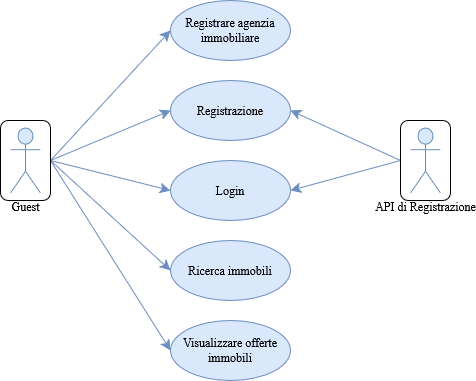
\includegraphics[width=0.8\textwidth]{Immagini/Diagrammi Casi D'uso/UseCase-Utente Non Registrato.drawio.png}
\end{figure}

\begin{figure}[H]
\centering
\caption{Casi d'uso Utente}
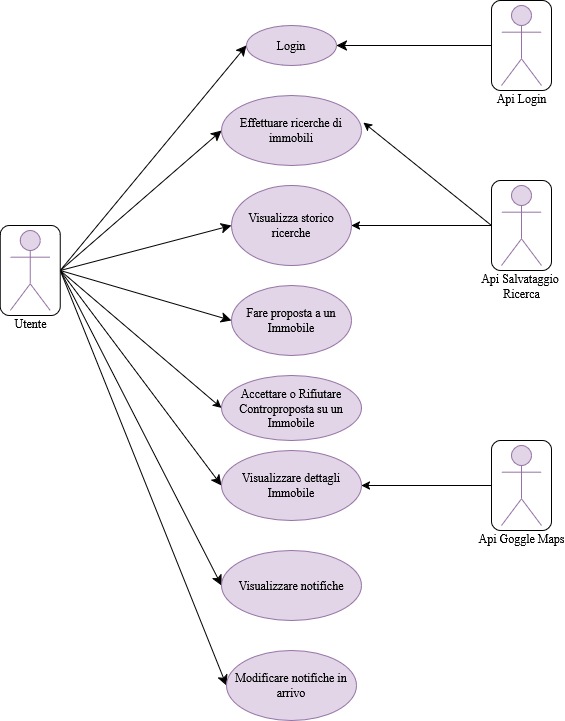
\includegraphics[width=0.8\textwidth]{Immagini/Diagrammi Casi D'uso/UseCase-Utente registrato.drawio.png}
\end{figure}

\begin{figure}[H]
\centering
\caption{Casi d'uso Agente}
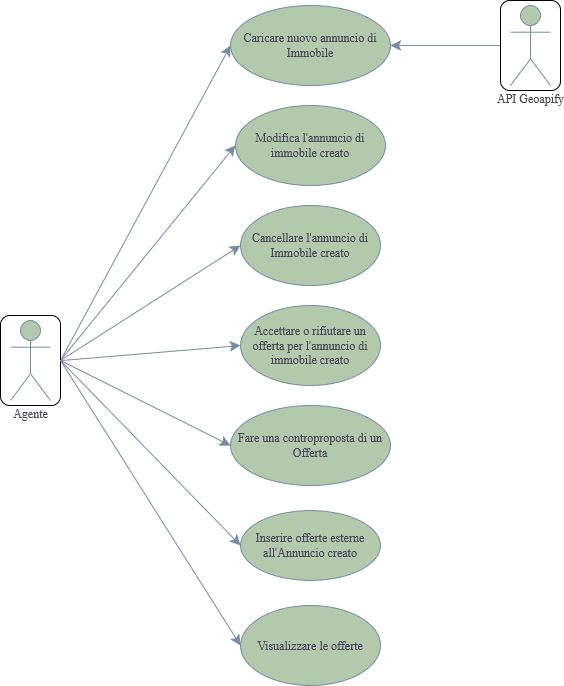
\includegraphics[width=0.8\textwidth]{Immagini/Diagrammi Casi D'uso/UseCase-Agente.drawio.png}
\end{figure}

\begin{figure}[H]
\centering
\caption{Casi d'uso Amministratore}
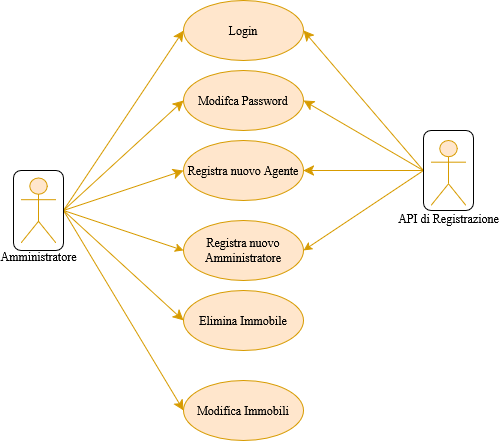
\includegraphics[width=0.8\textwidth]{Immagini/Diagrammi Casi D'uso/UseCase-Admin.drawio.png}
\end{figure}
\newpage

% punto c)
\section{Analisi Target Utenti
}
Quando si crea un software, è importante ricordare che non è necessario soddisfare ogni singolo utente possibile, ma solo la categoria di utenti che usufruiranno del nostra sistema più frequentemente.\\
Questa decisione ci permette di concentrare la nostra analisi e ridurre funzioni che, al momento del rilascio del software al committente, sono superflue.\\
Uno strumento utile per fare questa analisi è la 
Persona, un modello di utente ideale che può essere basato su ricerche di mercato oppure da input dai committenti stessi.\\
\subsection*{Personas Individuate}
Per creare Personas è stato adottato un approccio basato su ipotesi e ricerche secondarie.\\
Abbiamo così definito il contesto, identificando il pubblico target, i loro obiettivi e le situazioni in cui potrebbero utilizzare il prodotto. Si possono utilizzare archetipi comuni del dominio di riferimento per immaginare utenti tipo, discutendo possibili bisogni, obiettivi e preferenze degli utenti.\\
Abbiamo creato le Personas a partire da una template predefinita e usando Figma per il design e l'aggiornamento di esse in corso d'opera.
\\

\begin{figure}[H]
\centering
\caption{Proprietario Agenzia immobiliare}
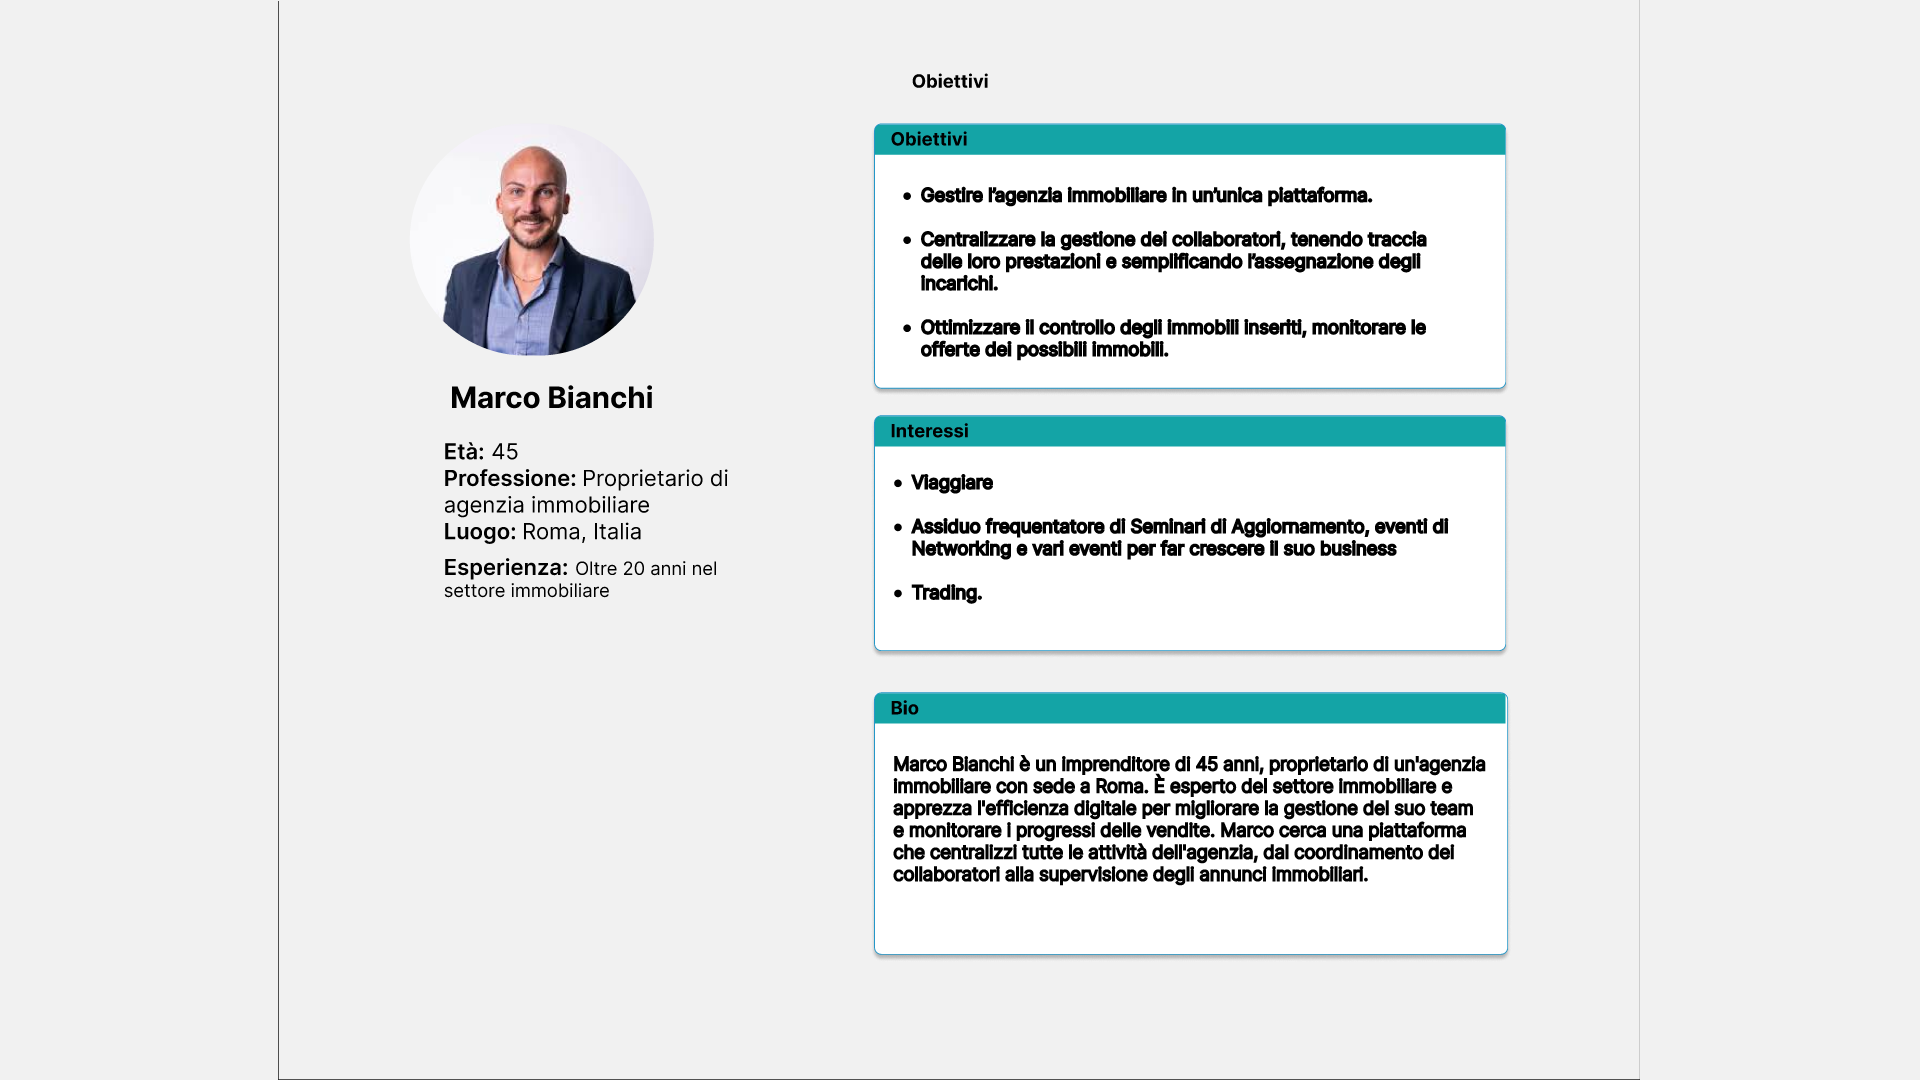
\includegraphics[width=1\textwidth]{{Immagini/Personas/Personas-Propretario di un agenzia immobiliare.png}}
\end{figure}

\begin{figure}[H]
\centering
\caption{Agente immobiliare}
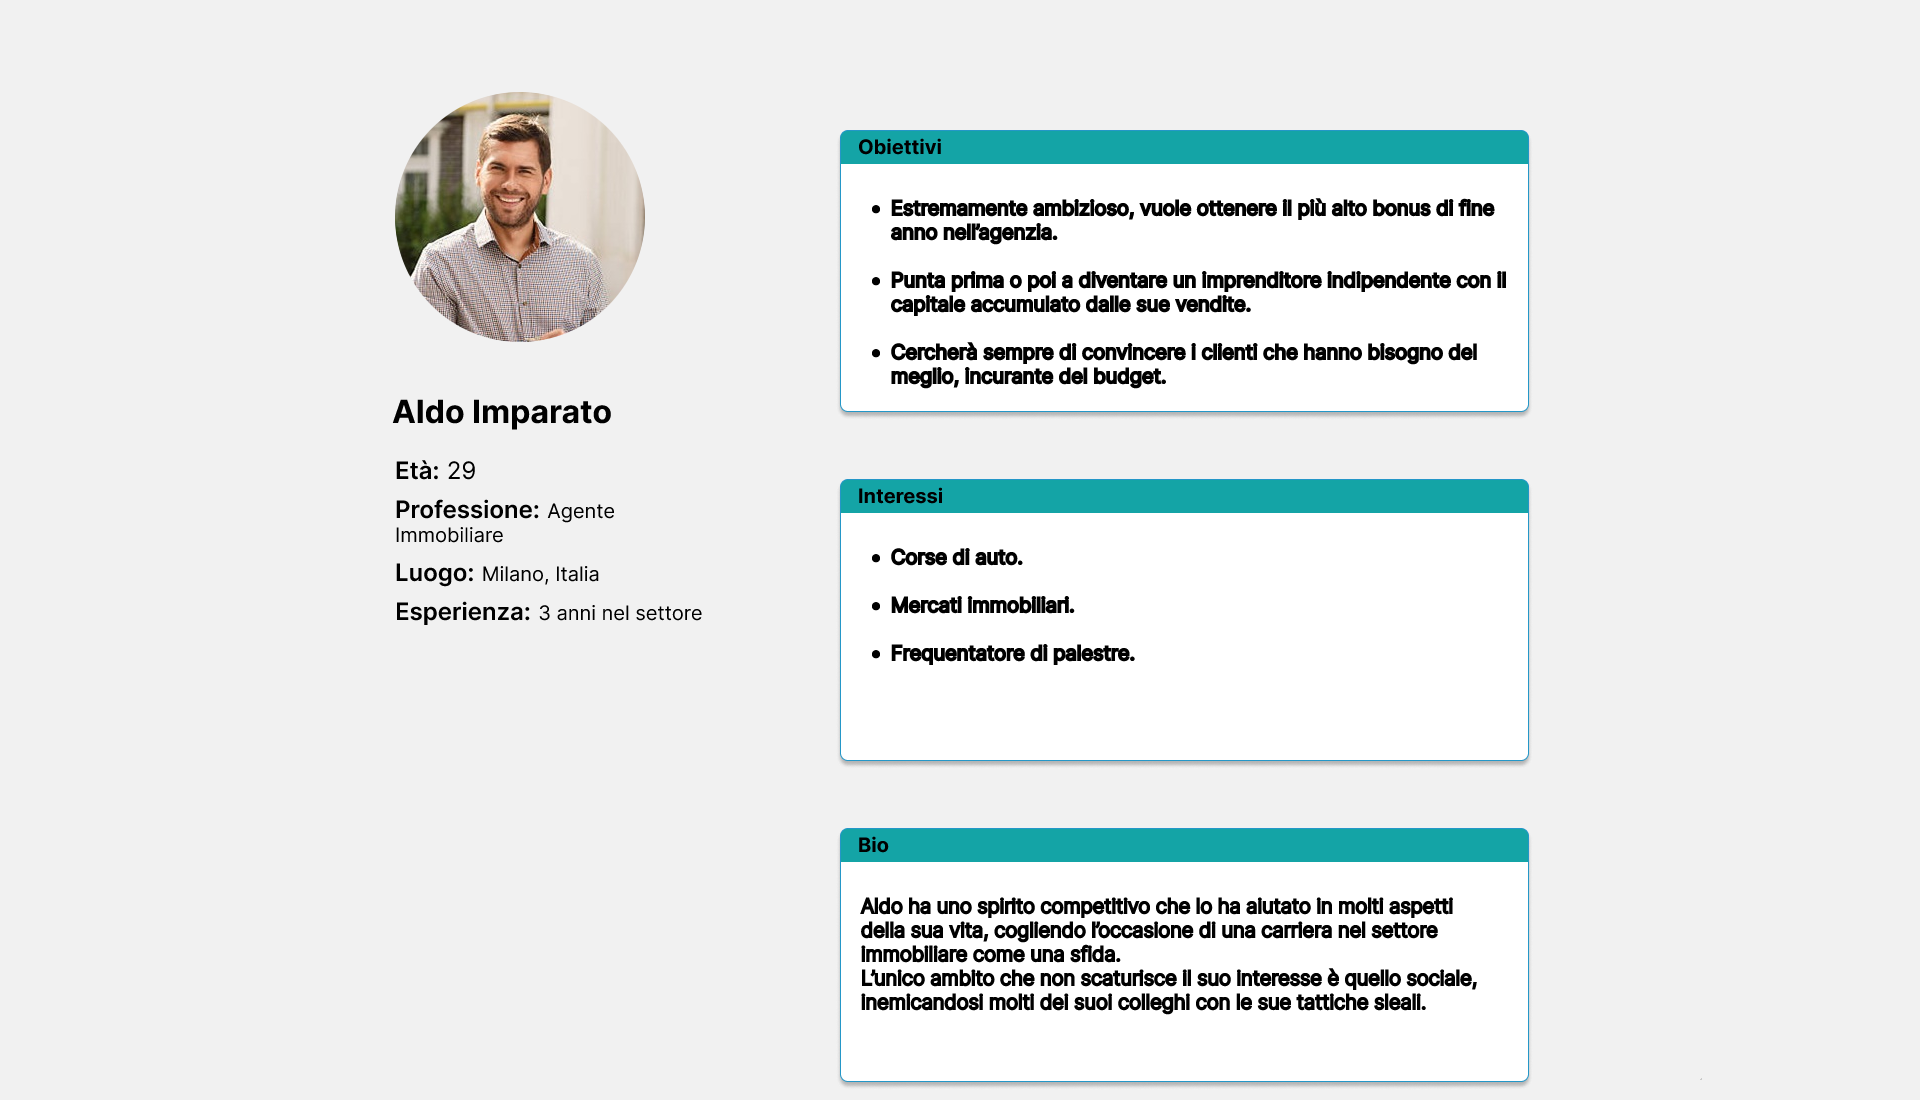
\includegraphics[width=1\textwidth]{{Immagini/Personas/Personas-Agente Immobiliare.png}}
\end{figure}

\begin{figure}[H]
\centering
\caption{Manager di azienda tecnologica}
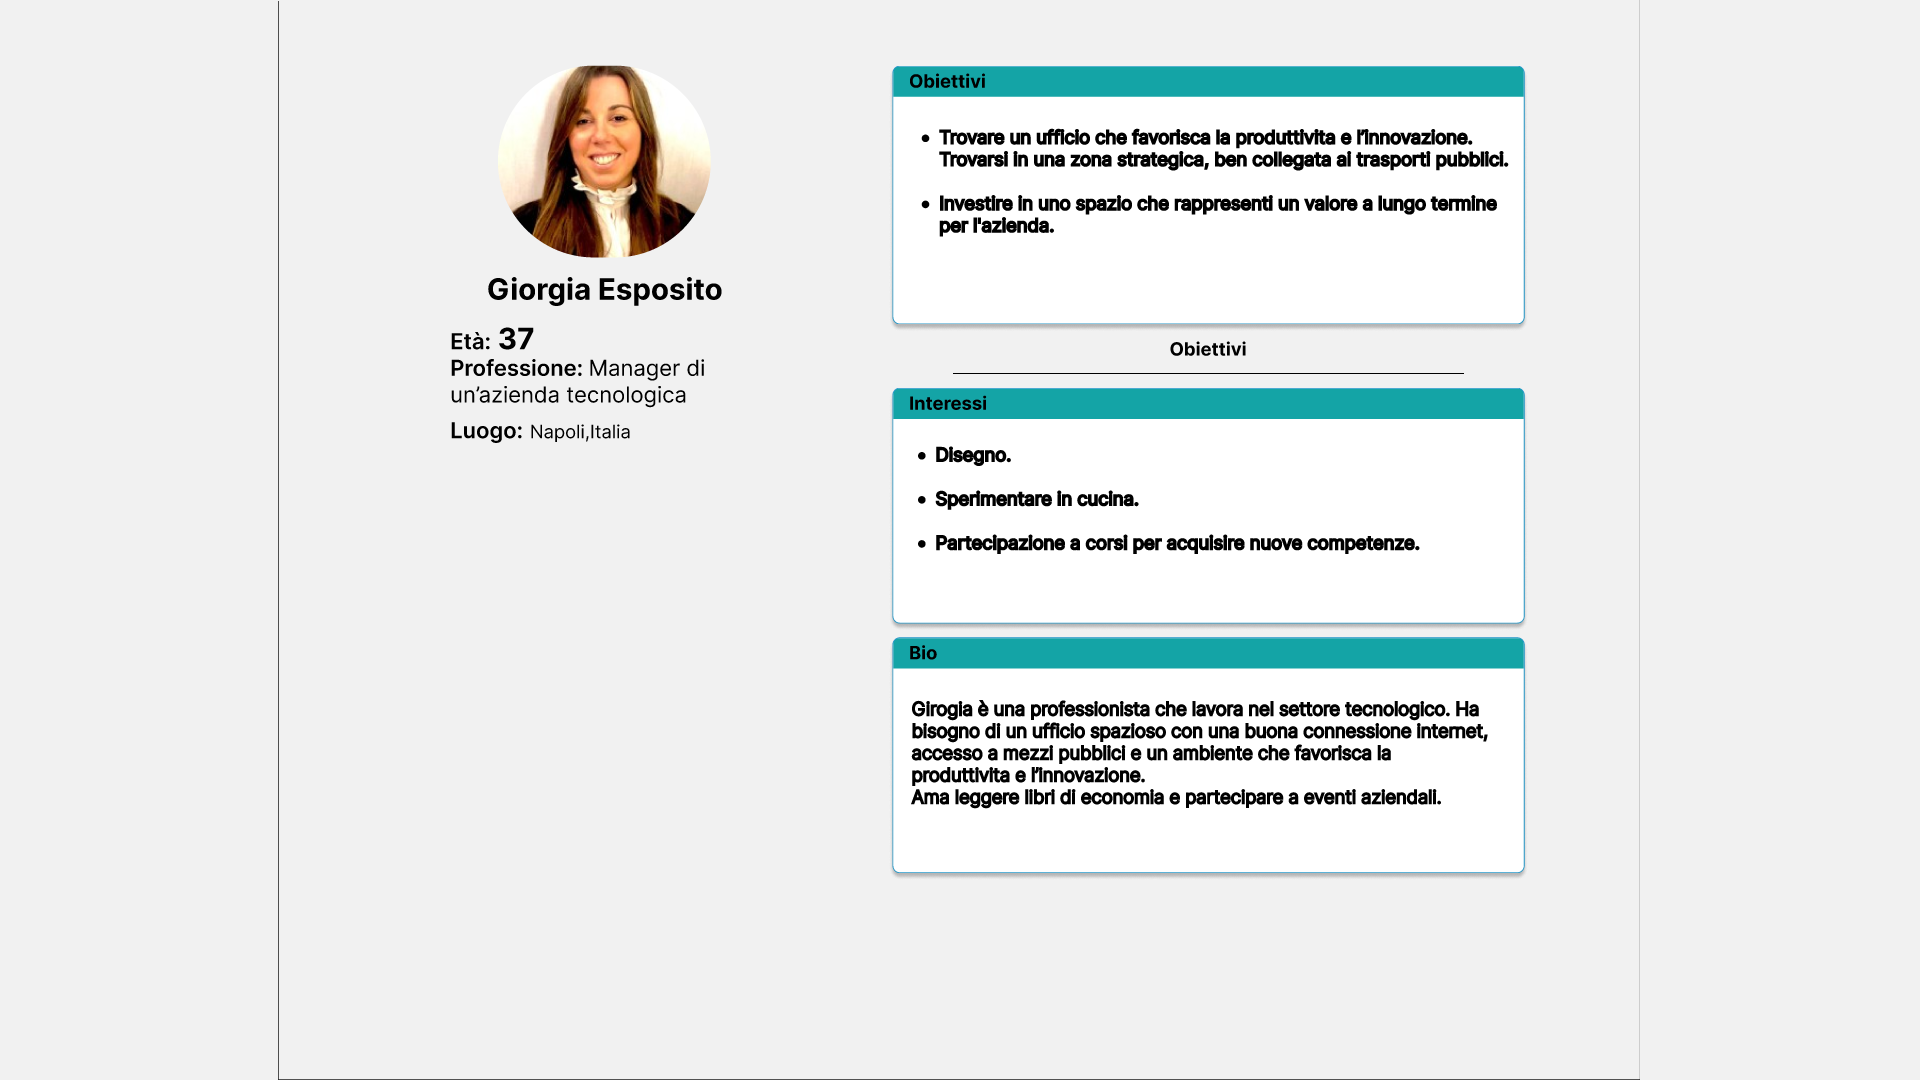
\includegraphics[width=1\textwidth]{Immagini/Personas/Personas-manager di azienda tecnologica.png}
\end{figure}

\begin{figure}[H]
\centering
\caption{Padre di famiglia}
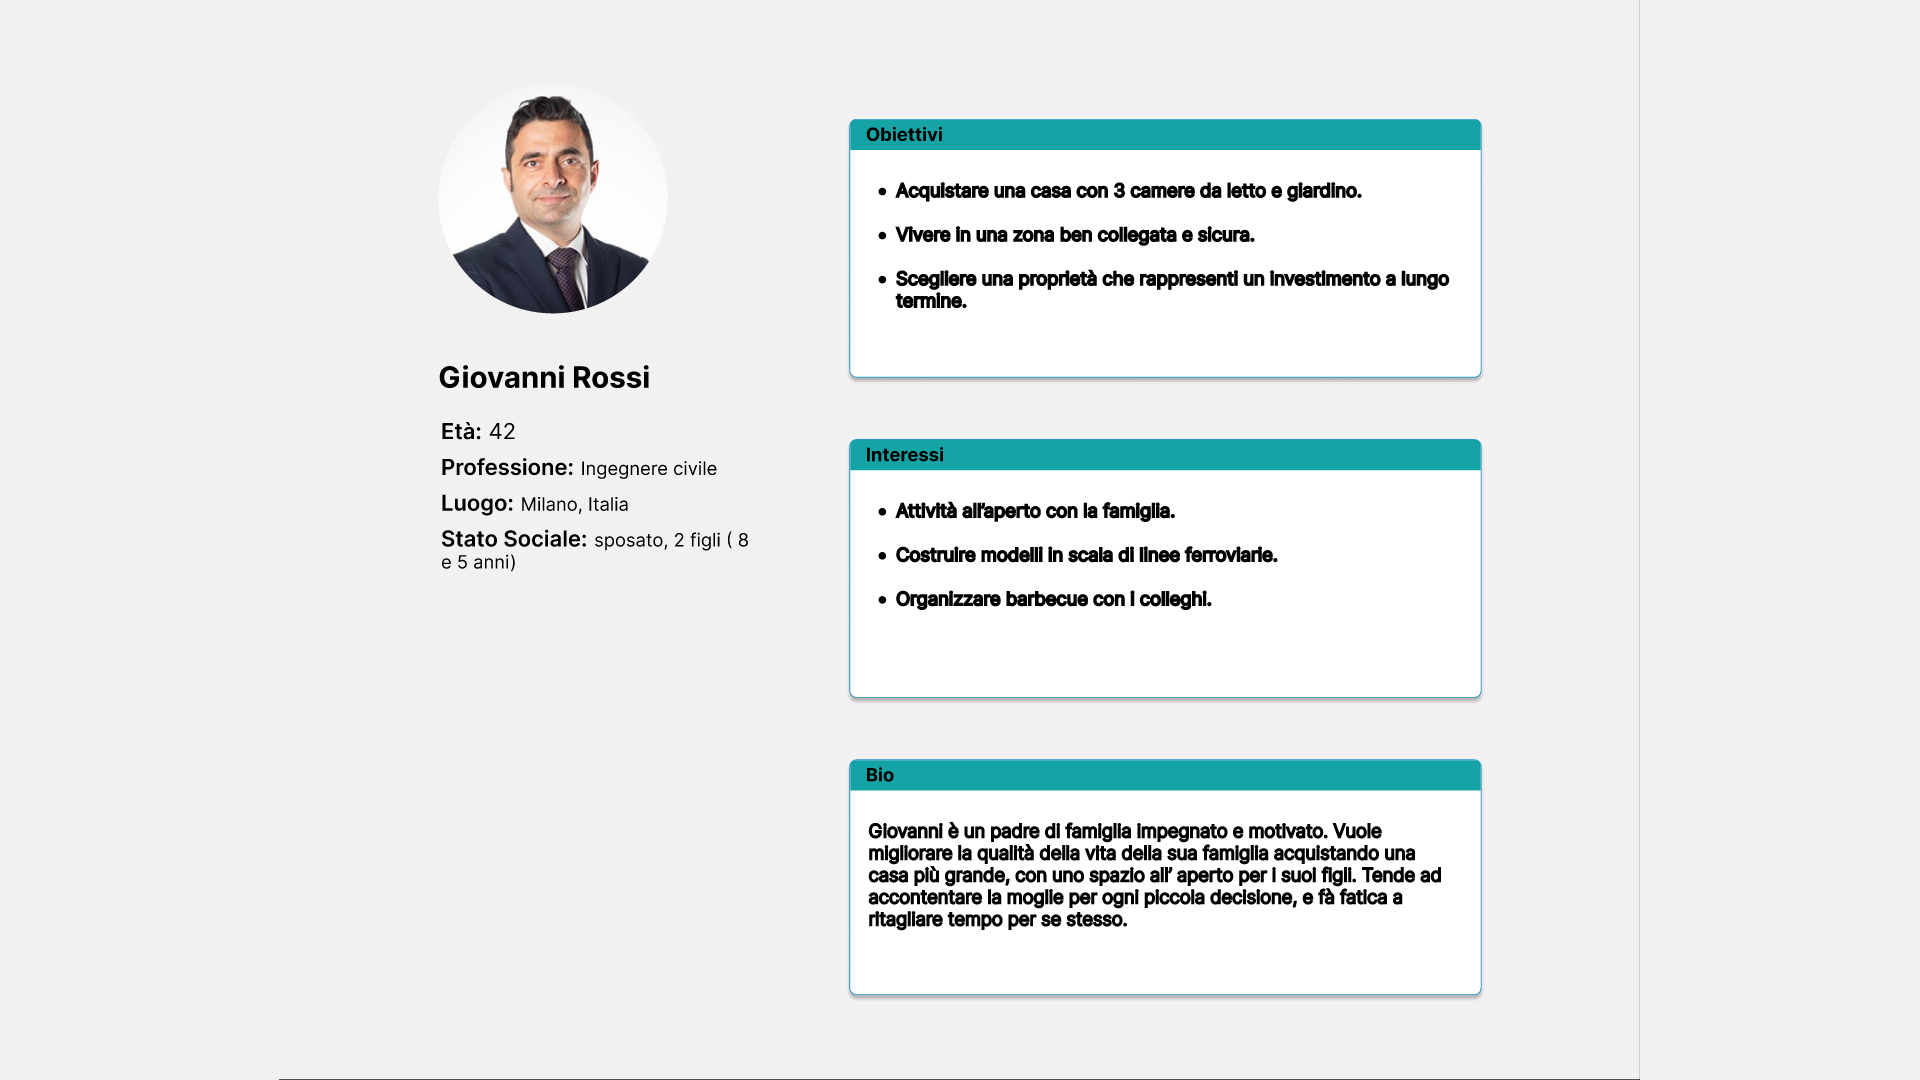
\includegraphics[width=1\textwidth]{Immagini/Personas/Personas-Padre di famiglia.png}
\end{figure}
\newpage
\subsection*{Tratti Caratteristici}
Analizzando queste Personas possiamo notare dei tratti che possiamo usare nella nostra applicazione:
\begin{itemize}
    \item  L'Agente- Aldo Imparato: questa categoria di utenti è parte dello staff dell'Agenzia immobiliare e quindi ha accesso al lato di amministrazione degli Immobili, e potrebbe volere una sezione nella sa pagina personale che gli mostra tutti gli Immobili a suo carico.
    \item  Il Padre di Famiglia - Giovanni Rossi: l'archetipo che incarna il Utente medio che ha vaghe idee su cosa vuole e si affida all'agente immobiliare. Dobbiamo quindi tener conto che le informazioni visibili a questo tipo di utenti deve essere chiara e concisa, come ad esempio le etichette che indicando punti di interesse come parchi e scuole.
    \item Il Manager di Azienda Tecnologica - Giorgia Esposito: l'utente che sta cercando qualcosa di ben definito, ma l'agenzia non offre Immobili con le caratteristiche cercate. Per questo tipo di persone offriremo un servizio di iscrizione ai tag di interesse per ricevere notifiche quando un immobile che rispecchia tali desideri viene messo in vendita.
    \item Il Proprietario dell'Agenzia Immobiliare - Marco Bianchi: gli amministratori del sistema che gestiscono dipendenti e il catalogo di Immobili, questo tipo di utente deve gestire multipli dati personali e sensibili. Quando crea un Agente o Amministratore, le nuove informazioni verranno generate dal sistema e inviate tramite un servizio di posta elettronica.
\end{itemize}
\newpage
% punto d)
\clearpage
\section{Descrizione Requisiti}

\subsection{Requisiti non funzionali}

\subsection*{Sicurezza}

\begin{table}[H]
    \centering
    \renewcommand{\arraystretch}{1.3} % Aumenta leggermente l'altezza delle righe
    
    \begin{tabular}{|p{3cm}|p{10cm}|} 
        \hline
        \textbf{ID} & \textbf{Descrizione} \\  
        \hline
        NF-S1 &  Implementazione di protocolli standard di sicurezza (es. HTTPS per il trasporto sicuro
        dei dati). \\ 
        \hline
        NF-S2 &  Le credenziali devono essere salvate in modo sicuro, utilizzando tecniche di hashing sicuro. \\ 
        \hline
        NF-S3 &  Le richieste alle REST API devono essere autenticate utilizzando JWT (JSON Web Tokens), per garantire che solo gli utenti autenticati possano accedere alle risorse protette. \\ 
        \hline
    \end{tabular}
    
\end{table}
\subsection*{Interfaccia utente}

\begin{table}[H]
    \centering
    \renewcommand{\arraystretch}{1.3} % Aumenta leggermente l'altezza delle righe
    \begin{tabular}{|p{3cm}|p{10cm}|} 
        \hline
        \textbf{ID} & \textbf{Descrizione} \\  
        \hline
        NF-UI11 & L'interfaccia utente deve adattarsi automaticamente alla risoluzione dello schermo dell’utente, garantendo un’esperienza di utilizzo ottimale su dispositivi mobili e desktop. \\ 
        \hline
    \end{tabular}
\end{table}
\subsection*{Prestazioni}

\begin{table}[H]
    \centering
    \renewcommand{\arraystretch}{1.3} % Aumenta leggermente l'altezza delle righe
    \begin{tabular}{|p{3cm}|p{10cm}|} 
        \hline
        \textbf{ID} & \textbf{Descrizione} \\  
        \hline
        NF-P1 & La ricerca e la visualizzazione degli immobili devono avere un tempo di risposta inferiore
        a 2 secondi, con un database contenente almeno 10.000 record. \\ 
        \hline
    \end{tabular}
\end{table}
\subsection*{Manutenibilità e scalabilità}

\begin{table}[H]
    \centering
    \renewcommand{\arraystretch}{1.3} % Aumenta leggermente l'altezza delle righe
    \begin{tabular}{|p{3cm}|p{10cm}|} 
        \hline
        \textbf{ID} & \textbf{Descrizione} \\  
        \hline
        NF-MS1 & Il sistema deve essere progettato per supportare l’aggiunta di nuove tipologie di immobili
        e contratti (ad esempio, affitti brevi) senza modificare l’architettura esistente. \\ 
        \hline
    \end{tabular}
\end{table}

\newpage

\subsection{Requisiti di dominio}

\subsection*{Gestione dell'agenzia immobiliare}

\begin{table}[H]
    \centering
    \renewcommand{\arraystretch}{1.3} % Aumenta leggermente l'altezza delle righe
    
    \begin{tabular}{|p{3cm}|p{10cm}|} 
        \hline
        \textbf{ID} & \textbf{Descrizione} \\  
        \hline
        D-A1 &  Un’agenzia immobiliare è composta da un fondatore e da una lista di dipendenti, ciascuno
        dei quali ricopre il ruolo di amministratore o agente immobiliare. \\ 
        \hline
        D-A2 &  La registrazione di un’agenzia immobiliare comporta la generazione automatica di un
        amministratore con il ruolo di fondatore. \\ 
        \hline
        D-A3 &  Alla creazione di un account amministratore vengono assegnate credenziali predefinite
        che possono essere modificate in seguito. \\ 
        \hline
        D-A4 &   Le credenziali di un amministratore includono uno username, costruito seguendo il formato [nome][cognome]@DIETI25.com, e una password scelta dall’utente. \\ 
        \hline
    \end{tabular}
    
\end{table}
\subsection*{Gestione degli utenti}

\begin{table}[H]
    \centering
    \renewcommand{\arraystretch}{1.3} % Aumenta leggermente l'altezza delle righe
    
    \begin{tabular}{|p{3cm}|p{10cm}|} 
        \hline
        \textbf{ID} & \textbf{Descrizione} \\  
        \hline
        D-U1 & Un guest può registrarsi al sistema fornendo un’email valida e una password, diventando così un utente. \\ 
        \hline
        D-U2 & Un guest può registrarsi o accedere tramite l’uso di API di terze parti. \\ 
        \hline
    \end{tabular}
    
\end{table}
\subsection*{Gestione degli immobili}

\begin{table}[H]
    \centering
    \renewcommand{\arraystretch}{1.3} % Aumenta leggermente l'altezza delle righe
    
    \begin{tabular}{|p{3cm}|p{10cm}|} 
        \hline
        \textbf{ID} & \textbf{Descrizione} \\  
        \hline
        D-G1 &  Ogni immobile è descritto da una serie di dettagli obbligatori, tra cui: foto, descrizione, prezzo, dimensioni, indirizzo, numero di stanze, piano, presenza di ascensore, classe energetica e ulteriori servizi (es. portineria, climatizzazione). \\ 
        \hline
        D-G2 &  Ogni immobile è associato a una delle seguenti tipologie contrattuali: "vendita" o "affitto". \\ 
        \hline
        D-G3 &  Ogni immobile, al momento della creazione, ha associata una lista di punti di riferimento generata automaticamente utilizzando il servizio GEOAPIFY. \\ 
        \hline
    \end{tabular}
    
\end{table}
\subsection*{Ricerca e visualizzazione}

\begin{table}[H]
    \centering
    \renewcommand{\arraystretch}{1.3} % Aumenta leggermente l'altezza delle righe
    
    \begin{tabular}{|p{3cm}|p{10cm}|} 
        \hline
        \textbf{ID} & \textbf{Descrizione} \\  
        \hline
        D-R1 &  La ricerca degli immobili consente di effettuare una selezione geografica basata su un punto centrale e un raggio, garantendo una precisione pari o superiore al 95\%. \\ 
        \hline
        D-R2 &  La ricerca avanzata degli immobili permette di utilizzare parametri multipli, tra cui tipologia di inserzione, prezzo minimo e massimo, numero di stanze, classe energetica e area geografica tramite mappa interattiva. \\ 
        \hline
        D-R3 &  Gli immobili ricercati possono essere visualizzati su una mappa interattiva. \\ 
        \hline
    \end{tabular}
    
\end{table}
\subsection*{Gestione delle offerte}

\begin{table}[H]
    \centering
    \renewcommand{\arraystretch}{1.3} % Aumenta leggermente l'altezza delle righe
    
    \begin{tabular}{|p{3cm}|p{10cm}|} 
        \hline
        \textbf{ID} & \textbf{Descrizione} \\  
        \hline
        D-O1 & Le inserzioni degli immobili possono ricevere offerte da parte degli utenti, composte da un prezzo proposto e dalle credenziali dell’offerente. Le offerte sono visibili a tutti gli utenti. \\ 
        \hline
    \end{tabular}
    
\end{table}
\subsection*{Gestione delle notifiche}

\begin{table}[H]
    \centering
    \renewcommand{\arraystretch}{1.3} % Aumenta leggermente l'altezza delle righe
    
    \begin{tabular}{|p{3cm}|p{10cm}|} 
        \hline
        \textbf{ID} & \textbf{Descrizione} \\  
        \hline
        D-N1 & Il sistema di notifiche consente di inviare avvisi personalizzati agli utenti, categorizzati in base a eventi come: nuove proprietà in linea con ricerche precedenti, conferme o rifiuti di proposte, e messaggi promozionali. \\ 
        \hline
        D-N2 & Le notifiche promozionali sono composte da un contenuto in formato RICH TEXT, definito dagli amministratori, e sono visibili esclusivamente agli utenti iscritti alla relativa newsletter. \\ 
        \hline
    \end{tabular}
    
\end{table}


% punto e. I)
\section{Descrizione Testuale strutturata del Sistema}
In questa sezione faremo un analisi più approfondita di alcuni dei casi d'uso campione del sistema, per esporre il nostro ragionamento per modellare e sviluppare il Software .\\
Questa descrizione ci servirà per pensare a che tipo di interazioni con l'Utente sono necessarie, i passaggi da effettuare  dal sistema in risposta alle richieste ricevute e 
I casi d'uso scelti per questo scopo sono la Creazione di un nuovo Annuncio di un Immobile e Modifica notifiche in Arrivo.
  
\subsection{Cockburn: nuovo annuncio}

\begin{figure}[H]
	\centering
	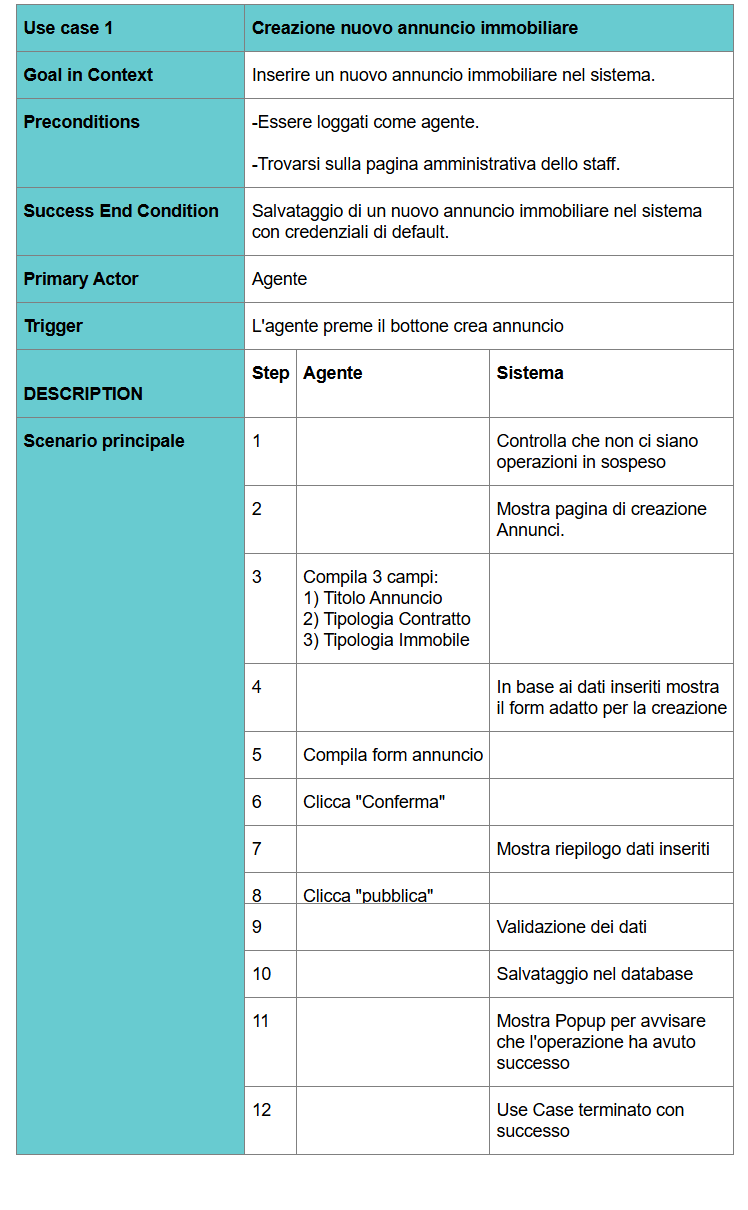
\includegraphics[width=1\linewidth]{"Immagini/cockburn/nuovo annuncio principale.png"}
	\caption[CockBurn extensions: registra nuovo annuncio]{}
	\label{fig:registra-nuovo-annuncio-principale}
\end{figure}

\newpage

\begin{figure}[H]
	\centering
	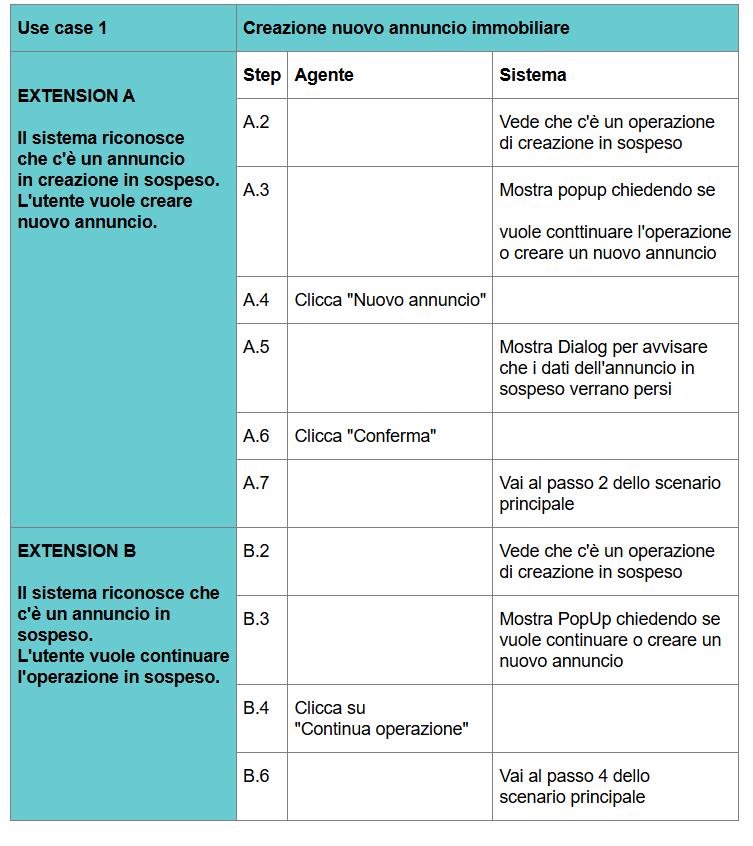
\includegraphics[width=1\linewidth]{"Immagini/cockburn/nuovo annuncio estensioni 1.png"}
	\caption[CockBurn extensions: registra nuovo annuncio]{}
	\label{fig:registra-nuovo-annuncio-extensions1}
\end{figure}

\newpage

\begin{figure}[H]
	\centering
	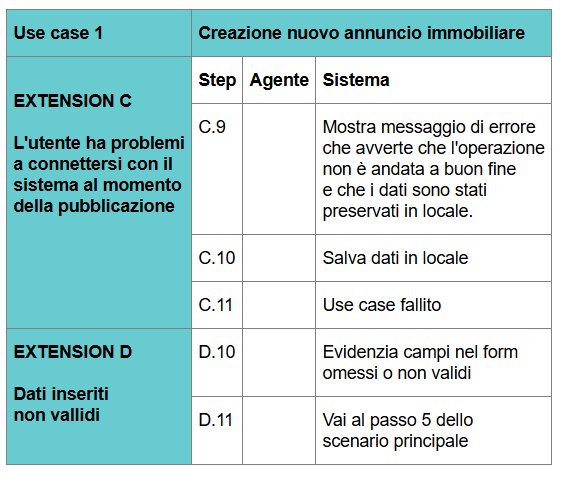
\includegraphics[width=1\linewidth]{"Immagini/cockburn/nuovo annuncio estensioni 2.png"}
	\caption[CockBurn extensions: registra nuovo annuncio]{}
	\label{fig:registra-nuovo-annuncio-extensions2}
\end{figure}
\newpage
% Please add the following required packages to your document preamble:
% \usepackage{multirow}
% \usepackage[table,xcdraw]{xcolor}
% Beamer presentation requires \usepackage{colortbl} instead of \usepackage[table,xcdraw]{xcolor}
% \usepackage{longtable}
% Note: It may be necessary to compile the document several times to get a multi-page table to line up properly
\begin{longtable}{|l|lll|}
\caption{}
\label{tab:my-table}\\
\hline
\rowcolor[HTML]{E1D5E7} 
\textbf{Use Case 2}                                                                                                                                                                 & \multicolumn{3}{l|}{\cellcolor[HTML]{E1D5E7}\textbf{Modifica notifiche in Arrivo}}                                                                                                                                                                                                                                                                                                                        \\ \hline
\endhead
%
\cellcolor[HTML]{E1D5E7}\textbf{Goal In Context}                                                                                                                                    & \multicolumn{3}{l|}{Cambia lo stato di notiche a scelta}                                                                                                                                                                                                                                                                                                                                                  \\ \hline
\cellcolor[HTML]{E1D5E7}\textbf{Preconditions}                                                                                                                                      & \multicolumn{3}{l|}{\begin{tabular}[c]{@{}l@{}}- Login effettuato con account con\\ ruolo Utente. \\ - Si trova nella pagina di Visualizazione notifiche\end{tabular}}                                                                                                                                                                                                                                    \\ \hline
\cellcolor[HTML]{E1D5E7}\textbf{\begin{tabular}[c]{@{}l@{}}Success End\\ Conditions\end{tabular}}                                                                                   & \multicolumn{3}{l|}{Lo stato di abilitazione di notifica viene modificato}                                                                                                                                                                                                                                                                                                                                \\ \hline
\cellcolor[HTML]{E1D5E7}\textbf{Primary Actor}                                                                                                                                      & \multicolumn{3}{l|}{Utente}                                                                                                                                                                                                                                                                                                                                                                               \\ \hline
\cellcolor[HTML]{E1D5E7}\textbf{Trigger}                                                                                                                                            & \multicolumn{3}{l|}{Utente preme il bottone Gestisci Notifiche}                                                                                                                                                                                                                                                                                                                                           \\ \hline
\rowcolor[HTML]{E1D5E7} 
\textbf{Descrizione}                                                                                                                                                                & \multicolumn{1}{l|}{\cellcolor[HTML]{E1D5E7}\textbf{Step n.}} & \multicolumn{1}{l|}{\cellcolor[HTML]{E1D5E7}\textbf{Utente}}                                                                            & \textbf{Sistema}                                                                                                                                                                                \\ \hline
\cellcolor[HTML]{E1D5E7}                                                                                                                                                            & \multicolumn{1}{l|}{1}                                        & \multicolumn{1}{l|}{}                                                                                                                   & \textit{\begin{tabular}[c]{@{}l@{}}Mostra pagina delle\\ notifiche\end{tabular}}                                                                                                                \\ \cline{2-4} 
\cellcolor[HTML]{E1D5E7}                                                                                                                                                            & \multicolumn{1}{l|}{2}                                        & \multicolumn{1}{l|}{\begin{tabular}[c]{@{}l@{}}Click Bottone per\\ modificare stato notifica\end{tabular}}                              &                                                                                                                                                                                                 \\ \cline{2-4} 
\cellcolor[HTML]{E1D5E7}                                                                                                                                                            & \multicolumn{1}{l|}{3}                                        & \multicolumn{1}{l|}{}                                                                                                                   & \textit{\begin{tabular}[c]{@{}l@{}}Mosta una Popup con \\ elenco di tutte le \\ categorie che possono \\ essere Modificate\end{tabular}}                                                        \\ \cline{2-4} 
\cellcolor[HTML]{E1D5E7}                                                                                                                                                            & \multicolumn{1}{l|}{4}                                        & \multicolumn{1}{l|}{\begin{tabular}[c]{@{}l@{}}Click su la casella/e \\ relativa/e alla categoria/e \\ da Modificare\end{tabular}}      & \textit{}                                                                                                                                                                                       \\ \cline{2-4} 
\cellcolor[HTML]{E1D5E7}                                                                                                                                                            & \multicolumn{1}{l|}{5}                                        & \multicolumn{1}{l|}{Click Bottone Conferma}                                                                                             & \textit{}                                                                                                                                                                                       \\ \cline{2-4} 
\cellcolor[HTML]{E1D5E7}                                                                                                                                                            & \multicolumn{1}{l|}{6}                                        & \multicolumn{1}{l|}{}                                                                                                                   & \textit{\begin{tabular}[c]{@{}l@{}}Mostra Dialog con \\ un messaggio che \\ avverte l'Utente \\ che non riceverà \\ più nuove Notifiche \\ relative alla \\ categoria selezionata\end{tabular}} \\ \cline{2-4} 
\cellcolor[HTML]{E1D5E7}                                                                                                                                                            & \multicolumn{1}{l|}{7}                                        & \multicolumn{1}{l|}{\begin{tabular}[c]{@{}l@{}}Click Bottone Conferma \\ nella Dialog\end{tabular}}                                     & \textit{}                                                                                                                                                                                       \\ \cline{2-4} 
\cellcolor[HTML]{E1D5E7}                                                                                                                                                            & \multicolumn{1}{l|}{8}                                        & \multicolumn{1}{l|}{}                                                                                                                   & \textit{\begin{tabular}[c]{@{}l@{}}Modifica Stato \\ Notifica in Database\end{tabular}}                                                                                                         \\ \cline{2-4} 
\cellcolor[HTML]{E1D5E7}                                                                                                                                                            & \multicolumn{1}{l|}{9}                                        & \multicolumn{1}{l|}{}                                                                                                                   & \textit{\begin{tabular}[c]{@{}l@{}}Feedback visivo del \\ cambio di visibilità\end{tabular}}                                                                                                    \\ \cline{2-4} 
\multirow{-50}{*}{\cellcolor[HTML]{E1D5E7}\textbf{\begin{tabular}[c]{@{}l@{}}Scenario \\ Principale\end{tabular}}}                                                                  & \multicolumn{1}{l|}{10}                                       & \multicolumn{1}{l|}{}                                                                                                                   & \textit{\begin{tabular}[c]{@{}l@{}}Use Case terminato \\ con Successo\end{tabular}}                                                                                                             \\ \hline
\newpage
\rowcolor[HTML]{E1D5E7} 
\textbf{Extension}                                                                                                                                                                  & \multicolumn{1}{l|}{\cellcolor[HTML]{E1D5E7}\textbf{Step n.}} & \multicolumn{1}{l|}{\cellcolor[HTML]{E1D5E7}\textbf{Utente}}                                                                            & \textbf{Sistema}                                                                                                                                                                                \\ \hline
\cellcolor[HTML]{E1D5E7}                                                                                                                                                            & \multicolumn{1}{l|}{A.2}                                      & \multicolumn{1}{l|}{click su notifica ricevuta}                                                                                         & \textit{}                                                                                                                                                                                       \\ \cline{2-4} 
\cellcolor[HTML]{E1D5E7}                                                                                                                                                            & \multicolumn{1}{l|}{A.3}                                      & \multicolumn{1}{l|}{}                                                                                                                   & \textit{\begin{tabular}[c]{@{}l@{}}Mostra il contenuto \\ della notifica\end{tabular}}                                                                                                          \\ \cline{2-4} 
\cellcolor[HTML]{E1D5E7}                                                                                                                                                            & \multicolumn{1}{l|}{A.4}                                      & \multicolumn{1}{l|}{\begin{tabular}[c]{@{}l@{}}Click Bottone Disattiva\\ Notifica\end{tabular}}                                         & \textit{}                                                                                                                                                                                       \\ \cline{2-4} 
\cellcolor[HTML]{E1D5E7}                                                                                                                                                            & \multicolumn{1}{l|}{A.5}                                      & \multicolumn{1}{l|}{}                                                                                                                   & \textit{\begin{tabular}[c]{@{}l@{}}Bottone\\ Disattiva Notifica \\ diventa Bottone \\ Attiva Notifica\end{tabular}}                                                                             \\ \cline{2-4} 

\multirow{-15}{*}{\cellcolor[HTML]{E1D5E7}\begin{tabular}[c]{@{}l@{}}Utente vuole \\ disabilitare una categoria \\ di notifiche a partire da \\ una notifica ricevuta\end{tabular}}    & \multicolumn{1}{l|}{A.6}                                      & \multicolumn{1}{l|}{}                                                                                                                   & \textit{\begin{tabular}[c]{@{}l@{}}Vai allo step 6 dello\\ Scenario Principale\end{tabular}}                                                                                                    \\ \hline
\cellcolor[HTML]{E1D5E7}                                                                                                                                                            & \multicolumn{1}{l|}{B.6}                                      & \multicolumn{1}{l|}{}                                                                                                                   & \textit{\begin{tabular}[c]{@{}l@{}}Il sistema nota che \\ non ci sono state \\ modifiche\end{tabular}}                                                                                          \\ \cline{2-4} 
\multirow{-4}{*}{\cellcolor[HTML]{E1D5E7}\begin{tabular}[c]{@{}l@{}}Utente non modifica \\ nessuna categoria \\ durante lo \\ Scenario Principale\end{tabular}}                     & \multicolumn{1}{l|}{B.7}                                      & \multicolumn{1}{l|}{}                                                                                                                   & \textit{\begin{tabular}[c]{@{}l@{}}Use case Terminato \\ con Successo\end{tabular}}                                                                                                             \\ \hline
\cellcolor[HTML]{E1D5E7}                                                                                                                                                            & \multicolumn{1}{l|}{C.2}                                      & \multicolumn{1}{l|}{\begin{tabular}[c]{@{}l@{}}Utente preme Bottone\\ Disabilita dalla lista delle\\ categorie Visibili\end{tabular}}   &                                                                                                                                                                                                 \\ \cline{2-4} 
\cellcolor[HTML]{E1D5E7}                                                                                                                                                            & \multicolumn{1}{l|}{C.3}                                      & \multicolumn{1}{l|}{}                                                                                                                   & \textit{\begin{tabular}[c]{@{}l@{}}Bottone Disabilita \\ diventa\\ Bottone Abilita\end{tabular}}                                                                                                \\ \cline{2-4} 
\multirow{-6}{*}{\cellcolor[HTML]{E1D5E7}\begin{tabular}[c]{@{}l@{}}Utente vuole disabilitare \\ categoria dalla lista \\ delle Categorie Attive\end{tabular}}                      & \multicolumn{1}{l|}{C.4}                                      & \multicolumn{1}{l|}{\textit{}}                                                                                                          & \textit{\begin{tabular}[c]{@{}l@{}}Vai al Passo 6 dello \\ Scenario Principale\end{tabular}}                                                                                                    \\ \hline
\cellcolor[HTML]{E1D5E7}                                                                                                                                                            & \multicolumn{1}{l|}{D.2}                                      & \multicolumn{1}{l|}{\begin{tabular}[c]{@{}l@{}}Utente Preme Bottone\\ Abilita dalla lista delle \\ Categorie disabilitate\end{tabular}} &                                                                                                                                                                                                 \\ \cline{2-4} 
\cellcolor[HTML]{E1D5E7}                                                                                                                                                            & \multicolumn{1}{l|}{D.3}                                      & \multicolumn{1}{l|}{}                                                                                                                   & \textit{\begin{tabular}[c]{@{}l@{}}Bottone Abilita \\ diventa\\ Bottone Disabilita\end{tabular}}                                                                                                \\ \cline{2-4} 
\multirow{-6}{*}{\cellcolor[HTML]{E1D5E7}\begin{tabular}[c]{@{}l@{}}Utente vuole abilitare\\ categoria dalla lista delle\\ Categorie Disabilitate\end{tabular}}                     & \multicolumn{1}{l|}{D.4}                                      & \multicolumn{1}{l|}{\textit{}}                                                                                                          & \textit{\begin{tabular}[c]{@{}l@{}}Vai al Passo 8 dello \\ Scenario Principale\end{tabular}}                                                                                                    \\ \hline
\cellcolor[HTML]{E1D5E7}                                                                                                                                                            & \multicolumn{1}{l|}{E.7}                                      & \multicolumn{1}{l|}{}                                                                                                                   & \textit{\begin{tabular}[c]{@{}l@{}}Mostra messaggio di \\ Errore il quale \\ avverte che \\ l'operazione non è \\ andata a buon fine.\end{tabular}}                                             \\ \cline{2-4} 
\cellcolor[HTML]{E1D5E7}                                                                                                                                                            & \multicolumn{1}{l|}{}                                         & \multicolumn{1}{l|}{}                                                                                                                   &                                                                                                                                                                                                 \\
\cellcolor[HTML]{E1D5E7}                                                                                                                                                            & \multicolumn{1}{l|}{}                                         & \multicolumn{1}{l|}{}                                                                                                                   &                                                                                                                                                                                                 \\
\multirow{-7}{*}{\cellcolor[HTML]{E1D5E7}\begin{tabular}[c]{@{}l@{}}Il sistema è Offline al \\ click del bottone \\ dell’Utente oppure \\ non è collegato a Internet.\end{tabular}} & \multicolumn{1}{l|}{\multirow{-3}{*}{E.8}}                    & \multicolumn{1}{l|}{\multirow{-3}{*}{}}                                                                                                 & \multirow{-3}{*}{\textit{\begin{tabular}[c]{@{}l@{}}Use Case Terminato \\ in Fallimento.\end{tabular}}}                                                                                         \\ \hline
\newpage
\cellcolor[HTML]{E1D5E7}                                                                                                                                                            & \multicolumn{1}{l|}{\cellcolor[HTML]{FFFFFF}F.2}              & \multicolumn{1}{l|}{Click su notifica ricevuta}                                                                                         & \textit{}                                                                                                                                                                                       \\ \cline{2-4} 
\cellcolor[HTML]{E1D5E7}                                                                                                                                                            & \multicolumn{1}{l|}{\cellcolor[HTML]{FFFFFF}F.3}              & \multicolumn{1}{l|}{}                                                                                                                   & \textit{\begin{tabular}[c]{@{}l@{}}Mostra il contenuto \\ della notifica\end{tabular}}                                                                                                          \\ \cline{2-4} 
\cellcolor[HTML]{E1D5E7}                                                                                                                                                            & \multicolumn{1}{l|}{\cellcolor[HTML]{FFFFFF}F.4}              & \multicolumn{1}{l|}{\begin{tabular}[c]{@{}l@{}}Click Bottone Attiva\\ Notifica\end{tabular}}                                            &                                                                                                                                                                                                 \\ \cline{2-4} 
\cellcolor[HTML]{E1D5E7}                                                                                                                                                            & \multicolumn{1}{l|}{F.5}                                      & \multicolumn{1}{l|}{}                                                                                                                   & \textit{\begin{tabular}[c]{@{}l@{}}Bottone \\ Attiva Notifiche\\ diventa Bottone \\ Disabilita Notifiche\end{tabular}}                                                                          \\ 

\cline{2-4} 
\multirow{-15}{*}{\cellcolor[HTML]{E1D5E7}\begin{tabular}[c]{@{}l@{}}Utente vuole abilitare \\ una categoria di \\ notifiche a partire \\ da una notica ricevuta\end{tabular}}       & \multicolumn{1}{l|}{\cellcolor[HTML]{FFFFFF}F.6}              & \multicolumn{1}{l|}{\cellcolor[HTML]{FFFFFF}\textbf{}}                                                                                  & \textit{\begin{tabular}[c]{@{}l@{}}Vai al Passo 8 dello \\ Scenario Principale\end{tabular}}                                                                                                    \\ \hline
\end{longtable}
\newpage
\subsection{Cockburn: Effettua controproposta di un'offerta}

\begin{figure}[H]
	\centering
	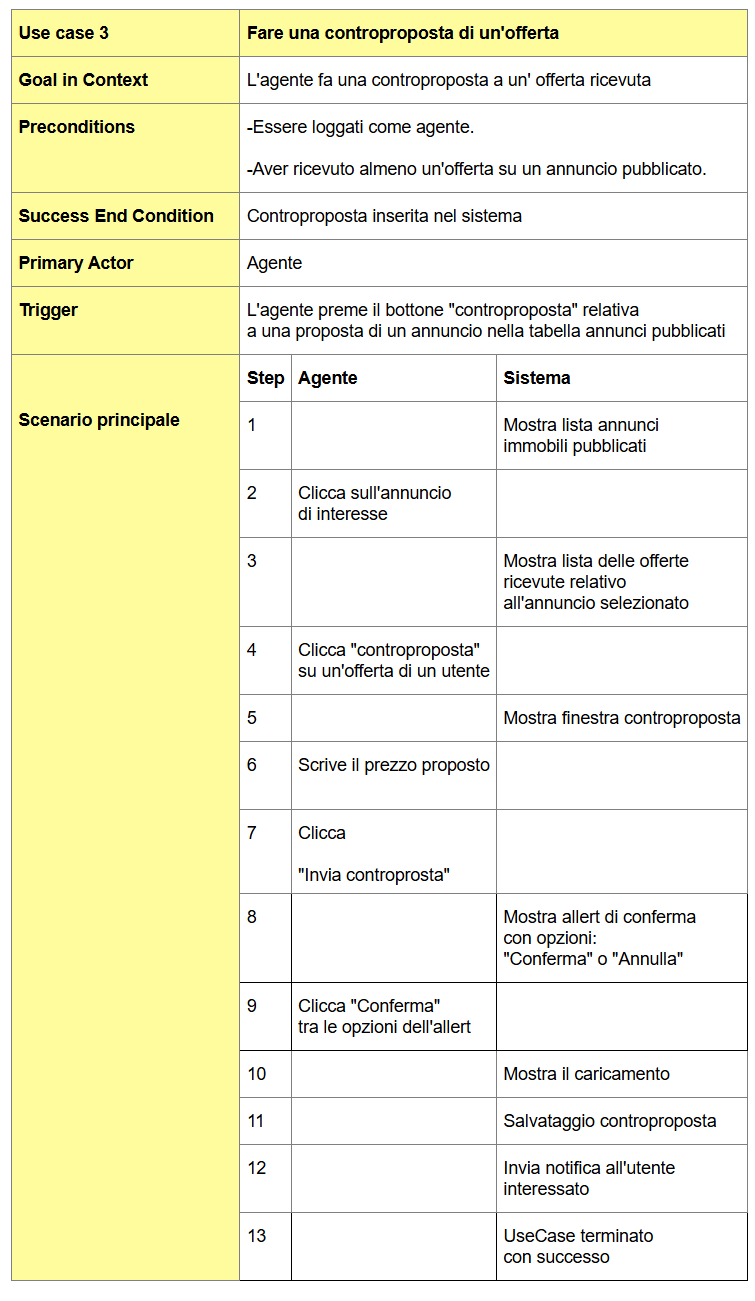
\includegraphics[width=0.8\linewidth]{"Immagini/cockburn/controproposta principale.png"}
	\caption[CockBurn extensions: registra nuovo agente]{}
	\label{fig:controproposta-principale}
\end{figure}

\newpage

\begin{figure}[H]
	\centering
	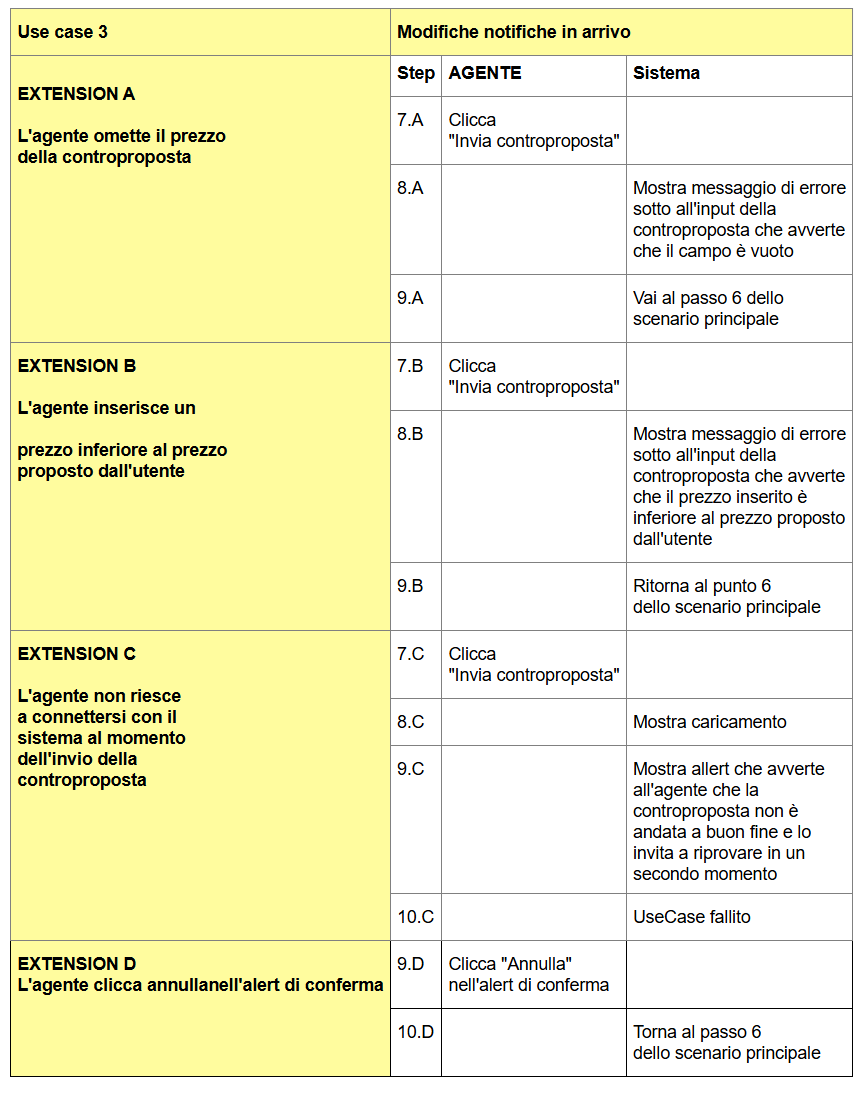
\includegraphics[width=1\linewidth]{"Immagini/cockburn/controproposta estensioni.png"}
	\caption[CockBurn extensions: registra nuovo agente]{}
	\label{fig:controproposta-estensioni}
\end{figure}
\newpage
\subsection{Cockburn: Registra nuovo agente} 

\begin{table}[H]
	\begin{tabular}{|
			>{\columncolor[HTML]{9AFF99}}l |lll|}
		\hline
		\textbf{Use case 4}                                            & \multicolumn{3}{l|}{\cellcolor[HTML]{9AFF99}\textbf{Registra nuovo agente}}                                                                                                                                                                                           \\ \hline
		Goal in Context                                                & \multicolumn{3}{l|}{Inserire un nuovo agente di un agenzia immobiliare nel sistema.}                                                                                                                                                                                  \\ \hline
		Preconditions                                                  & \multicolumn{3}{l|}{\begin{tabular}[c]{@{}l@{}}-Essere loggati come agente.\\ \\ -Aver ricevuto almeno un offerta su un \\ immobile pubblicato.\end{tabular}}                                                                                                         \\ \hline
		Success End Condition                                          & \multicolumn{3}{l|}{Salvataggio di un nuovo agente nel sistema con credenziali di default.}                                                                                                                                                                           \\ \hline
		DESCRIPTION                                                    & \multicolumn{1}{l|}{\textbf{Step}} & \multicolumn{1}{l|}{\textbf{Manager}}                                                                          & \textbf{Sistema}                                                                                                \\ \hline
		\cellcolor[HTML]{9AFF99}                                       & \multicolumn{1}{l|}{1}             & \multicolumn{1}{l|}{\begin{tabular}[c]{@{}l@{}}Clicca \\ “Registra nuovo dipendente”\end{tabular}}             &                                                                                                                 \\ \cline{2-4} 
		\cellcolor[HTML]{9AFF99}                                       & \multicolumn{1}{l|}{2}             & \multicolumn{1}{l|}{}                                                                                          & \begin{tabular}[c]{@{}l@{}}Mostra pagina \\ registrazione dipendente\end{tabular}                               \\ \cline{2-4} 
		\cellcolor[HTML]{9AFF99}                                       & \multicolumn{1}{l|}{3}             & \multicolumn{1}{l|}{\begin{tabular}[c]{@{}l@{}}Compila form\\ selezionando "Agente"\\ come ruolo\end{tabular}} &                                                                                                                 \\ \cline{2-4} 
		\cellcolor[HTML]{9AFF99}                                       & \multicolumn{1}{l|}{4}             & \multicolumn{1}{l|}{Clicca "Registra dipendente"}                                                              &                                                                                                                 \\ \cline{2-4} 
		\cellcolor[HTML]{9AFF99}                                       & \multicolumn{1}{l|}{5}             & \multicolumn{1}{l|}{}                                                                                          & \begin{tabular}[c]{@{}l@{}}Mostra allert di conferma\\ con opzioni\\ "Annulla" e "Conferma"\end{tabular}        \\ \cline{2-4} 
		\cellcolor[HTML]{9AFF99}                                       & \multicolumn{1}{l|}{6}             & \multicolumn{1}{l|}{Clicca "Conferma"}                                                                         &                                                                                                                 \\ \cline{2-4} 
		\cellcolor[HTML]{9AFF99}                                       & \multicolumn{1}{l|}{7}             & \multicolumn{1}{l|}{}                                                                                          & Mostra caricamento                                                                                              \\ \cline{2-4} 
		\cellcolor[HTML]{9AFF99}                                       & \multicolumn{1}{l|}{8}             & \multicolumn{1}{l|}{}                                                                                          & Genera credenziali di default                                                                                   \\ \cline{2-4} 
		\cellcolor[HTML]{9AFF99}                                       & \multicolumn{1}{l|}{9}             & \multicolumn{1}{l|}{}                                                                                          & \begin{tabular}[c]{@{}l@{}}Salvataggio nuovo agente\\ nel sistema con\\ credenziali di default\end{tabular}     \\ \cline{2-4} 
		\cellcolor[HTML]{9AFF99}                                       & \multicolumn{1}{l|}{10}            & \multicolumn{1}{l|}{}                                                                                          & \begin{tabular}[c]{@{}l@{}}Mostra messaggio di conferma\\ con allegato le credenziali di\\ default\end{tabular} \\ \cline{2-4} 
		\multirow{-11}{*}{\cellcolor[HTML]{9AFF99}Scenario principale} & \multicolumn{1}{l|}{11}            & \multicolumn{1}{l|}{}                                                                                          & \begin{tabular}[c]{@{}l@{}}Use case terminato\\ con successo\end{tabular}                                       \\ \hline
	\end{tabular}
\end{table}

\newpage

\begin{table}[H]
	\begin{tabular}{
			>{\columncolor[HTML]{9AFF99}}l lll}
		\hline
		\textbf{Use case 4}                                                                                                                                                                                                                                                                                 & \multicolumn{3}{l}{\cellcolor[HTML]{9AFF99}\textbf{Registra nuovo agente}}                                                                                                                                                                   \\ \hline
		\multicolumn{1}{|l|}{\cellcolor[HTML]{9AFF99}}                                                                                                                                                                                                                                                      & \multicolumn{1}{l|}{\textbf{Step}} & \multicolumn{1}{l|}{\textbf{Manager}}              & \multicolumn{1}{l|}{\textbf{Sistema}}                                                                                                              \\ \cline{2-4} 
		\multicolumn{1}{|l|}{\cellcolor[HTML]{9AFF99}}                                                                                                                                                                                                                                                      & \multicolumn{1}{l|}{4.A}           & \multicolumn{1}{l|}{Clicca  “Registra dipendente”} & \multicolumn{1}{l|}{}                                                                                                                              \\ \cline{2-4} 
		\multicolumn{1}{|l|}{\cellcolor[HTML]{9AFF99}}                                                                                                                                                                                                                                                      & \multicolumn{1}{l|}{5.A}           & \multicolumn{1}{l|}{}                              & \multicolumn{1}{l|}{\begin{tabular}[c]{@{}l@{}}Mostra errori \\ nei campi non\\ compilati correttamente\end{tabular}}                              \\ \cline{2-4} 
		\multicolumn{1}{|l|}{\multirow{-4}{*}{\cellcolor[HTML]{9AFF99}\textbf{\begin{tabular}[c]{@{}l@{}}EXTENSION A\\ \\ Non tutti i campi\\ sono compilati\\ oppure compilati\\ correttamente\end{tabular}}}}                                                                                             & \multicolumn{1}{l|}{6.A}           & \multicolumn{1}{l|}{}                              & \multicolumn{1}{l|}{\begin{tabular}[c]{@{}l@{}}Ritorna al passo 3 dello\\ scenario principale\end{tabular}}                                        \\ \hline
		\multicolumn{1}{|l|}{\cellcolor[HTML]{9AFF99}{\color[HTML]{000000} }}                                                                                                                                                                                                                               & \multicolumn{1}{l|}{6.B}           & \multicolumn{1}{l|}{Clicca "Conferma"}             & \multicolumn{1}{l|}{}                                                                                                                              \\ \cline{2-4} 
		\multicolumn{1}{|l|}{\cellcolor[HTML]{9AFF99}{\color[HTML]{000000} }}                                                                                                                                                                                                                               & \multicolumn{1}{l|}{7.B}           & \multicolumn{1}{l|}{}                              & \multicolumn{1}{l|}{Mostra caricamento}                                                                                                            \\ \cline{2-4} 
		\multicolumn{1}{|l|}{\cellcolor[HTML]{9AFF99}{\color[HTML]{000000} }}                                                                                                                                                                                                                               & \multicolumn{1}{l|}{8.B}           & \multicolumn{1}{l|}{}                              & \multicolumn{1}{l|}{\begin{tabular}[c]{@{}l@{}}Il sistema genera automaticamente\\ un email alternativa che aggiunge\\ un id univoco\end{tabular}} \\ \cline{2-4} 
		\multicolumn{1}{|l|}{\multirow{-4}{*}{\cellcolor[HTML]{9AFF99}{\color[HTML]{000000} \textbf{\begin{tabular}[c]{@{}l@{}}EXTENSION B\\ \\ Il manager tenta\\ di registrare un\\ agente il cui nome\\ e cognome sono\\ in comune con\\ un altro agente già\\ registato nel \\ sistema\end{tabular}}}}} & \multicolumn{1}{l|}{9.B}           & \multicolumn{1}{l|}{}                              & \multicolumn{1}{l|}{\begin{tabular}[c]{@{}l@{}}Ritorna al passo 9 dello\\ scenario principale\end{tabular}}                                        \\ \hline
		\multicolumn{1}{|l|}{\cellcolor[HTML]{9AFF99}}                                                                                                                                                                                                                                                      & \multicolumn{1}{l|}{6.C}           & \multicolumn{1}{l|}{Clicca "Annulla"}              & \multicolumn{1}{l|}{}                                                                                                                              \\ \cline{2-4} 
		\multicolumn{1}{|l|}{\multirow{-2}{*}{\cellcolor[HTML]{9AFF99}\textbf{\begin{tabular}[c]{@{}l@{}}EXTENSION C\\ \\ Clicca "Annulla"\\ invece di\\ "Conferma" nell'\\ allert di conferma\end{tabular}}}}                                                                                              & \multicolumn{1}{l|}{7.C}           & \multicolumn{1}{l|}{}                              & \multicolumn{1}{l|}{\begin{tabular}[c]{@{}l@{}}Ritorna al passo 3 dello\\ scenario principale\end{tabular}}                                        \\ \hline
		\multicolumn{1}{|l|}{\cellcolor[HTML]{9AFF99}}                                                                                                                                                                                                                                                      & \multicolumn{1}{l|}{6.D}           & \multicolumn{1}{l|}{Clicca "Conferma"}             & \multicolumn{1}{l|}{}                                                                                                                              \\ \cline{2-4} 
		\multicolumn{1}{|l|}{\cellcolor[HTML]{9AFF99}}                                                                                                                                                                                                                                                      & \multicolumn{1}{l|}{7.D}           & \multicolumn{1}{l|}{}                              & \multicolumn{1}{l|}{Mostra caricamento}                                                                                                            \\ \cline{2-4} 
		\multicolumn{1}{|l|}{\cellcolor[HTML]{9AFF99}}                                                                                                                                                                                                                                                      & \multicolumn{1}{l|}{8.D}           & \multicolumn{1}{l|}{}                              & \multicolumn{1}{l|}{\begin{tabular}[c]{@{}l@{}}Avvisa l'utente dell'operazione\\ fallita per motivi tecnici\end{tabular}}                          \\ \cline{2-4} 
		\multicolumn{1}{|l|}{\multirow{-4}{*}{\cellcolor[HTML]{9AFF99}\textbf{\begin{tabular}[c]{@{}l@{}}EXTENSION D\\ \\ L'utente non \\ riesce a connettersi\\ con il sistema\end{tabular}}}}                                                                                                             & 9.D                                &                                                    & User case fallito                                                                                                                                  \\ \hline
	\end{tabular}
\end{table}
% punto e.II)
\newpage
\section{Mock up e motivazioni dell’interfaccia utente adottata}
\subsection*{Introduzione}
Dopo aver definito gli use case utilizzando il metodo Cockburn, siamo passati alla fase di progettazione visiva realizzando una serie di mockup interattivi in Figma. Questi mockup hanno lo scopo di rappresentare graficamente le interazioni dell'utente con il sistema, traducendo le specifiche funzionali in un'interfaccia visibile e navigabile. Ogni mockup è stato sviluppato tenendo conto delle diverse casistiche previste negli use case e nelle loro estensioni, in modo da garantire un’esperienza utente coerente e intuitiva.

Nei paragrafi seguenti verranno presentati i vari mockup, suddivisi per use case. Ogni sezione illustrerà le scelte progettuali effettuate, evidenziando come la UI si adatti alle diverse situazioni previste dai casi d'uso.

\subsection{Caso d'Uso: Aggiungi un Annuncio Immobiliare}

Per garantire un’esperienza utente ottimale, abbiamo progettato i mockup del caso d'uso \textit{Aggiungi un Annuncio Immobiliare} seguendo i principi della user experience (UX) e dell'usabilità. Il percorso utente è stato studiato attentamente per minimizzare il carico cognitivo e semplificare l’interazione, in linea con i modelli proposti da Nielsen e Norman \cite{nielsen1995,norman1988}.

\subsection*{Schermata Iniziale: Gestione Annunci Immobiliari}
L’azione di aggiungere un nuovo annuncio parte dalla schermata di Gestione Annunci Immobiliari, dove l’utente trova:
\begin{itemize}
    \item \textbf{Una lista degli immobili a lui associati}, che consente una rapida contestualizzazione.
    \item \textbf{Un pulsante unico ed evidente}, etichettato “Aggiungi Annuncio Immobiliare”, che centralizza l’azione primaria.
\end{itemize}

\subsection*{Flusso di Navigazione e Segmentazione del Form}
Al click del pulsante, l’utente viene indirizzato a una schermata dedicata alla compilazione di un form articolato in più step. Questa segmentazione si basa sul principio del \textbf{chunking dell’informazione} \cite{miller1956}, riducendo il carico di memoria e rendendo il processo meno gravoso. In particolare:
\begin{itemize}
    \item \textbf{Step 1:} Richiede le informazioni basilari, quali il titolo, il tipo di contratto e il tipo di immobile.
    \item \textbf{Step 2 e successivi:} Raccolgono i dati principali e le caratteristiche secondarie dell’immobile, organizzati in modo logico e intuitivo.
\end{itemize}

\subsection*{Navigazione Sticky e Accessibilità degli Step}
I pulsanti di navigazione, posizionati in alto con comportamento \textit{sticky}, consentono all’utente di passare agevolmente da uno step all’altro, anche in presenza di schermate particolarmente lunghe. Tale scelta:
\begin{itemize}
    \item Riduce il tempo necessario per individuare i controlli di navigazione.
    \item Favorisce un’interazione continua e fluida, in linea con i principi di design centrato sull’utente e le best practice in ambito HCI (Human-Computer Interaction) \cite{shneiderman2004}.
\end{itemize}

\subsection*{Integrazione della Mappa Interattiva}
Per quanto riguarda l’inserimento dell’indirizzo:
\begin{itemize}
    \item \textbf{La mappa interattiva} permette di visualizzare immediatamente la posizione indicata, offrendo un feedback visivo diretto.
    \item L’utente ha la possibilità di regolare la posizione direttamente sulla mappa, migliorando la precisione del dato inserito \cite{wickens2008}.
\end{itemize}

\subsection*{Gestione delle Immagini e Feedback Visivo}
La sezione dedicata alle immagini è progettata per:
\begin{itemize}
    \item \textbf{Consentire l’aggiunta di foto} tramite pulsante dedicato o drag and drop, facilitando l’upload in maniera intuitiva.
    \item \textbf{Permettere l’inserimento di una descrizione} per ogni immagine, migliorando la contestualizzazione visiva dell’annuncio \cite{pieters2004}.
\end{itemize}

\subsection*{Anteprima e Conferma Finale}
Infine, viene presentato uno schema riepilogativo che funge da anteprima dell’annuncio così come apparirà agli utenti finali. Una volta verificata la correttezza dei dati:
\begin{itemize}
    \item L’utente può cliccare il pulsante \textbf{“Pubblica”}, che innesca un processo di caricamento e validazione.
    \item Al termine del processo, viene mostrato un messaggio di conferma che attesta il successo dell’operazione, riducendo l’ansia da incertezza e rafforzando la fiducia nel sistema \cite{nielsen1995}.
\end{itemize}

\newpage

\input{Requisiti Del Software/Analisi dei Requisiti/Mockup/aggiungi annuncio/scenario principale}

\input{Requisiti Del Software/Analisi dei Requisiti/Mockup/aggiungi annuncio/scenario principale Parte II}

\input{Requisiti Del Software/Analisi dei Requisiti/Mockup/aggiungi annuncio/estensione A}

\input{Requisiti Del Software/Analisi dei Requisiti/Mockup/aggiungi annuncio/estensione B}


\input{Requisiti Del Software/Analisi dei Requisiti/Mockup/aggiungi annuncio/estensione C}

\input{Requisiti Del Software/Analisi dei Requisiti/Mockup/aggiungi annuncio/estensione D}

\clearpage
\newpage

\subsection{Caso d'Uso: Attivazione e Disattivazione Notifiche}

Il sistema prevede un'interfaccia dedicata alla gestione delle preferenze di notifica, pensata per permettere all'utente di curare la propria esperienza d'uso dell'applicazione, ricevendo news solo sugli argomenti di interesse.\\
In questa sezione andremo a esaminare le scelte effettuate durante la progettazione, l'impatto sull'esperienza utente e i prototipi generati alla fine dell'analisi. 

\vspace{0.5cm}
\subsubsection{Tipologie di Notifiche e Controllo Utente}
Le notifiche sono suddivise in diverse categorie per permettere una personalizzazione granulare:
\begin{itemize}
    \item \textbf{Annunci di nuovi immobili}: notifiche basate sulle ricerche dell’utente.
    \item \textbf{Risposte alle offerte}: aggiornamenti sulle interazioni con gli annunci pubblicati.
    \item \textbf{Messaggi promozionali}: comunicazioni di marketing e offerte esclusive.
\end{itemize}
L’utente può, in qualsiasi momento, disattivare le notifiche per una o più categorie, mantenendo un controllo totale sulla propria esperienza \cite{shneiderman2004}.

\vspace{0.5cm}
\subsubsection{Gestione delle Notifiche e Conferma delle Modifiche}
La gestione delle notifiche avviene principalmente attraverso la schermata delle notifiche, composta da:
\begin{itemize}
    \item \textbf{Lista delle notifiche ricevute}, ognuna cliccabile per visualizzare i dettagli.
    \item \textbf{Barra laterale con le categorie di notifiche}, suddivise in:
    \begin{itemize}
        \item \textbf{Categorie attive}, con notifiche attualmente abilitate.
        \item \textbf{Categorie disattivate}, che non inviano più notifiche.
    \end{itemize}
\end{itemize}

In cima alla barra laterale è presente un’icona che, se cliccata, apre una schermata popup intitolata “Attiva e Disattiva Notifiche”. All’interno, ogni categoria è rappresentata da un toggle switch che indica lo stato attuale delle notifiche.

\vspace{0.5cm}
\subsubsection{Feedback Visivo e Animazioni Intuitive}
Per garantire un’interazione chiara e immediata, il sistema utilizza diverse tecniche di UX design:
\begin{itemize}
    \item \textbf{Animazione di transizione}: quando un toggle viene modificato, la categoria si sposta visivamente tra la sezione attiva e quella disattiva, sfruttando il principio di \textbf{gestalt della continuità} \cite{miller1956} per rendere il cambiamento intuitivo.
    \item \textbf{Feedback visivo immediato}: l’utente percepisce immediatamente l’effetto dell’azione senza necessità di un testo esplicativo eccessivo.
\end{itemize}

\newpage
\subsubsection{Conferma e Implicazioni della Disattivazione}
Per evitare errori accidentali e garantire consapevolezza delle conseguenze, la disattivazione di una categoria di notifiche è accompagnata da:
\begin{itemize}
    \item Un popup di conferma che informa l’utente che, durante il periodo in cui le notifiche sono disattivate, le notifiche non potranno essere recuperate \cite{wickens2008}.
    \item Un ulteriore messaggio di avviso prima della conferma definitiva, in linea con le \textbf{heuristiche di usabilità di Nielsen} \cite{nielsen1995} per la prevenzione degli errori.
\end{itemize}

Solo dopo la conferma finale, il sistema applica le modifiche alle preferenze dell'utente, garantendo un'interazione consapevole e trasparente.\\
Nel prototipo questi comportamenti sono stati modellati con un pulsante, tuttavia nell'applicazione finale è stato deciso di sostituirlo con un menù contestuale.



\input{Requisiti Del Software/Analisi dei Requisiti/Mockup/disattivazione notifiche/Scenario principale}

\input{Requisiti Del Software/Analisi dei Requisiti/Mockup/disattivazione notifiche/estensione A}
\input{Requisiti Del Software/Analisi dei Requisiti/Mockup/disattivazione notifiche/estensione B}

\input{Requisiti Del Software/Analisi dei Requisiti/Mockup/disattivazione notifiche/estensione c}

\input{Requisiti Del Software/Analisi dei Requisiti/Mockup/disattivazione notifiche/estensione D}

\input{Requisiti Del Software/Analisi dei Requisiti/Mockup/disattivazione notifiche/estensione E}

\input{Requisiti Del Software/Analisi dei Requisiti/Mockup/disattivazione notifiche/estensione F}


\subsection{Caso d'Uso: Controproposta di un'Offerta}

Il caso d’uso Controproposta di un’offerta è stato progettato seguendo la stessa logica di interazione non intrusiva adottata per altre operazioni simili.
L’obiettivo principale è mantenere la continuità del contesto visivo, riducendo al minimo le interruzioni nel flusso di lavoro dell’utente. Per questo motivo, l’azione viene gestita all’interno di una finestra modale (popup) che consente di operare senza abbandonare la vista principale.

\vspace{0.5cm}
\subsubsection{Struttura e Flusso dell’Interazione}
L’interazione si articola in più fasi distinte, ognuna delle quali mira a garantire chiarezza e controllo all’utente:
\begin{itemize}
	\item \textbf{Popup iniziale}: la finestra modale mostra i dettagli della proposta selezionata (mittente, testo sintetico e valore corrente) e include un campo dedicato all’inserimento del nuovo valore della controproposta.
	In calce è presente un pulsante di azione principale con etichetta \textbf{«Invia controproposta»}.
	
	\item \textbf{Conferma dell’invio}: al clic su \textbf{«Invia controproposta»}, viene visualizzato un dialog di conferma per prevenire invii accidentali.  
	I pulsanti di conferma e annullamento sono caratterizzati da colori neutri, così da differenziarli visivamente dalle azioni primarie della piattaforma e migliorare la leggibilità percettiva \cite{nielsen1995}.
	
	\item \textbf{Feedback di caricamento}: dopo la conferma, il sistema mostra una barra di avanzamento stilizzata con i colori istituzionali dell’applicazione.  
	Anche in presenza di tempi di risposta brevi, viene introdotto un lieve ritardo percettivo per garantire un feedback visivo chiaro sull’elaborazione in corso \cite{shneiderman2004}.
	
	
\end{itemize}

\vspace{0.5cm}
\subsubsection{Esito dell’Operazione e Aggiornamento della Lista}
Al completamento dell’operazione, il sistema applica una serie di aggiornamenti automatici per riflettere lo stato corrente:
\begin{itemize}
	\item la finestra modale viene chiusa automaticamente;
	\item nella lista delle proposte, la voce corrispondente viene aggiornata con il nuovo valore della controproposta;
	\item il testo della proposta precedente può essere troncato o sintetizzato per preservare la leggibilità complessiva della tabella;
	\item lo stato della proposta viene aggiornato a \emph{«Controproposta inviata»}, rendendo immediatamente visibile l’esito dell’azione.
\end{itemize}

\vspace{0.5cm}
\subsubsection{Considerazioni di Usabilità e Sicurezza}
La soluzione basata su finestra modale garantisce un’esperienza utente coerente con i principi di usabilità e sicurezza dell’interfaccia:
\begin{itemize}
	\item \textbf{Continuità contestuale}: l’utente rimane all’interno del proprio flusso operativo, con possibilità di annullamento rapido.
	\item \textbf{Prevenzione degli errori}: la doppia conferma riduce il rischio di invii accidentali, in linea con le \textbf{heuristiche di Nielsen} per la prevenzione degli errori \cite{nielsen1995}.
	\item \textbf{Feedback percettivo affidabile}: la barra di caricamento fornisce un riscontro visivo chiaro sullo stato del processo, migliorando la percezione di controllo dell’utente \cite{wickens2008}.
\end{itemize}

Dal punto di vista della gestione dei dati, è raccomandata la validazione \textit{server-side} del valore della controproposta e l’applicazione di politiche di accesso coerenti con i principi di \textbf{minimizzazione delle informazioni} e \textbf{sicurezza dei dati}.
In caso di errore di invio, il sistema deve presentare messaggi chiari e impedire l’invio ripetuto della stessa controproposta fino al completamento dell’elaborazione, prevenendo possibili condizioni di \textit{race} o incongruenze nei dati.

\begin{figure}[H]
	\centering
	\begin{tikzpicture}[node distance=1.5cm and 1cm, auto]
		% Nodo per immagine 1 con didascalia sotto
		\node (img1) {
			\begin{tabular}{c}
				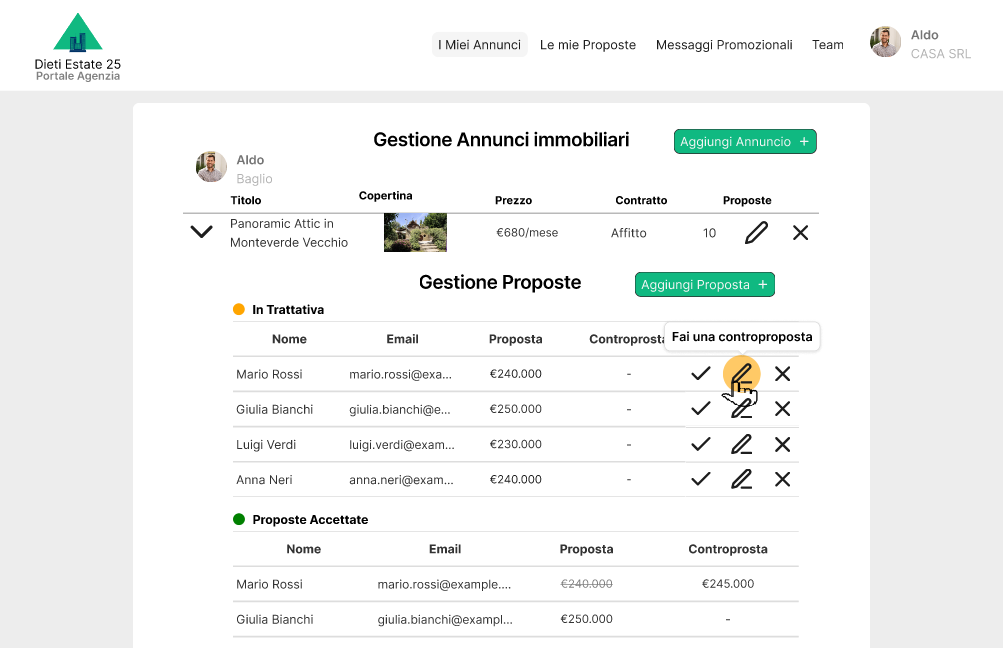
\includegraphics[width=0.7\textwidth]{Immagini/Mockup/controproposte/scenario principale/clickControproposta.png} \\
				Cockburn: step 1/2/3/4
			\end{tabular}
		};
		
		% Nodo per immagine 2 con didascalia sotto, posizionato a destra di img1
		\node (img2) [below=of img1] {
			\begin{tabular}{c}
				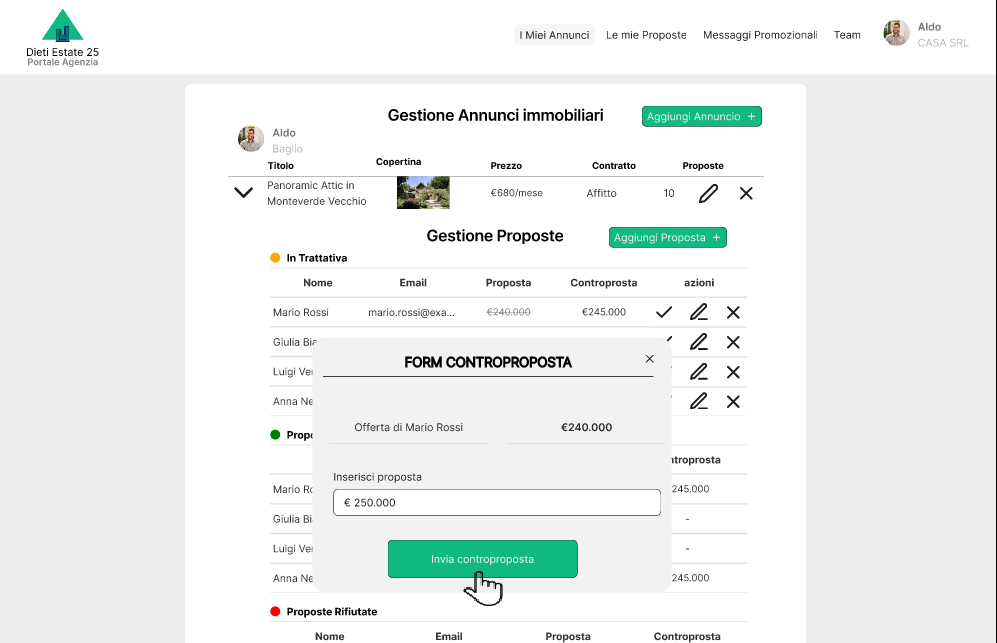
\includegraphics[width=0.7\textwidth]{Immagini/Mockup/controproposte/scenario principale/ClickInviaControproposta.png} \\
				Cockburn: step 5/6/7
			\end{tabular}
		};
		
		% Nodo per immagine 3 con didascalia sotto, posizionato sotto img2
		\node (img3) [below=of img2] {
			\begin{tabular}{c}
				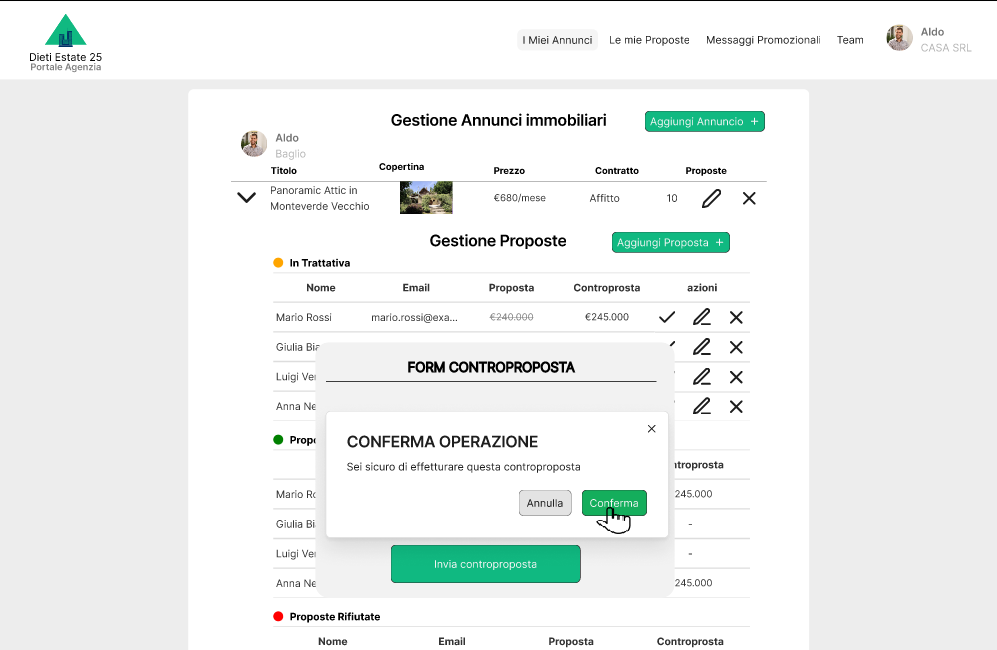
\includegraphics[width=0.7\textwidth]{Immagini/Mockup/controproposte/scenario principale/allertConfermaInvio.png} \\
				Cockburn: step 8/9/10
			\end{tabular}
		};
		
		% Disegna le frecce
		\draw[->, thick] (img1) -- (img2);
		\draw[->, thick] (img2) -- (img3);
		
	\end{tikzpicture}
	\caption{Mockup: scenario principale della tabella di Cockburn del caso d'uso: Fare una controproposta a un'offerta.}
	\label{fig:tikz_flow}
\end{figure}

\newpage

\begin{figure}[H]
	\centering
	\includegraphics[width=0.7\linewidth]{"Immagini/Mockup/controproposte/scenario principale/visualizzazioneControproposta"}
	\caption[Visualizzazione della controproposta]{}
	\label{fig:visualizzazionecontroproposta}
\end{figure}

\input{Requisiti Del Software/Analisi dei Requisiti/Mockup/controproposta/MockUp Controproposta extensions A}

\newpage

\input{Requisiti Del Software/Analisi dei Requisiti/Mockup/controproposta/MockUp Controproposta extensions B}

\newpage

\input{Requisiti Del Software/Analisi dei Requisiti/Mockup/controproposta/MockUp Controproposta extensions C}

\input{Requisiti Del Software/Analisi dei Requisiti/Mockup/controproposta/MockUp Controproposta extensions D}

\clearpage
\newpage



\subsection{Caso d'Uso: Registrazione di un Nuovo Agente}

Il caso d’uso «Registra nuovo agente» è stato progettato con l’obiettivo di garantire un’esperienza utente fluida e coerente con il resto dell’interfaccia, evitando interruzioni del contesto visivo. Per questo motivo, si è scelto di non introdurre una schermata dedicata, ma di utilizzare una finestra modale (popup), che consente all’utente di eseguire l’operazione senza abbandonare la vista corrente.

\vspace{0.5cm}
\subsubsection{Struttura e Flusso dell’Interazione}
L’interazione si articola in più fasi, guidando l’utente in modo progressivo e controllato:
\begin{itemize}
	\item \textbf{Popup iniziale}: contiene un form per l’inserimento dei dati anagrafici e professionali dell’agente, accompagnato da un unico pulsante in calce con etichetta «Registra nuovo utente».
	\item \textbf{Conferma dell’operazione}: al clic sul pulsante, viene mostrato un \textit{dialog} di doppia conferma per ridurre il rischio di azioni involontarie. I pulsanti di conferma e annullamento sono caratterizzati da colori neutri, in modo da distinguerli visivamente dall’azione primaria dell’applicazione.
	\item \textbf{Feedback di caricamento}: dopo la conferma, il sistema mostra una barra di avanzamento stilizzata con i colori istituzionali del sito. Anche nei casi in cui l’operazione risulti immediata, la barra può essere mantenuta visibile per una breve durata, al fine di fornire un riscontro percettivo chiaro e rassicurante \cite{nielsen1995}.
\end{itemize}

\vspace{0.5cm}
\subsubsection{Messaggio di Conferma e Gestione delle Credenziali}
Al completamento del processo di registrazione, il sistema visualizza un messaggio di successo che informa l’utente dell’avvenuta generazione delle credenziali di accesso.
Il pulsante contestuale assume l’etichetta \textbf{«Copia credenziali»}, permettendo di salvare in modo sicuro i dati generati.
Per prevenire la perdita delle credenziali, la chiusura del dialog è temporaneamente disabilitata fino a quando l’utente non conferma l’avvenuta copia.

\vspace{0.5cm}
\subsubsection{Visualizzazione e Sicurezza dei Dati}
In linea con i principi di \textbf{minimizzazione dei dati} e \textbf{sicurezza dell’informazione} \cite{wickens2008}, la visualizzazione completa delle credenziali non è obbligatoria:
il sistema privilegia la protezione dei dati sensibili, evitando di esporre informazioni in chiaro nell’interfaccia.
In alternativa, è possibile prevedere una versione mascherata delle credenziali o la sola visualizzazione di elementi non sensibili, mantenendo comunque la trasparenza informativa per l’utente.
\begin{figure}[H]
	\centering
	\begin{tikzpicture}[node distance=1.5cm and 1cm, auto]
		% Nodo per immagine 1 con didascalia sotto
		\node (img1) {
			\begin{tabular}{c}
				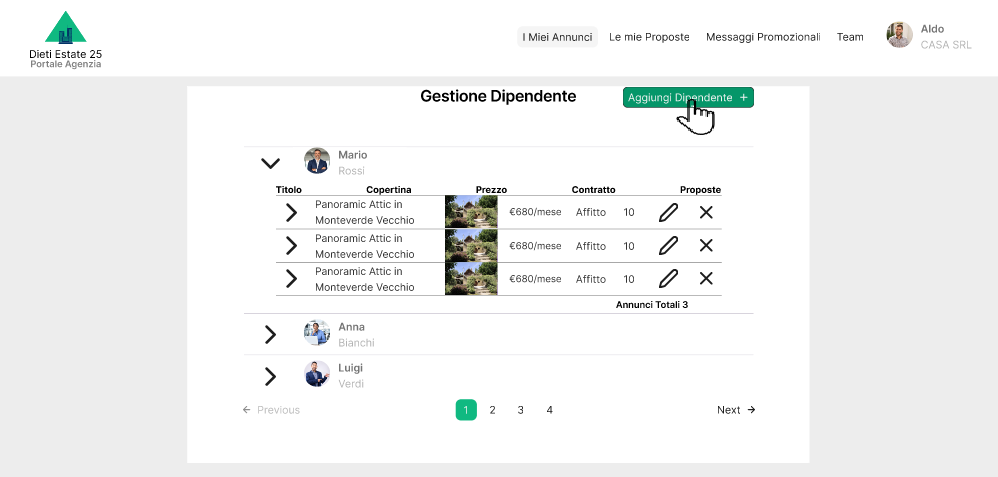
\includegraphics[width=0.7\textwidth]{Immagini/Mockup/nuovoAgente/scenario principale/clickNuovoDipendente.png} \\
				Cockburn: step 1
			\end{tabular}
		};
		
		% Nodo per immagine 2 con didascalia sotto, posizionato a destra di img1
		\node (img2) [below=of img1] {
			\begin{tabular}{c}
				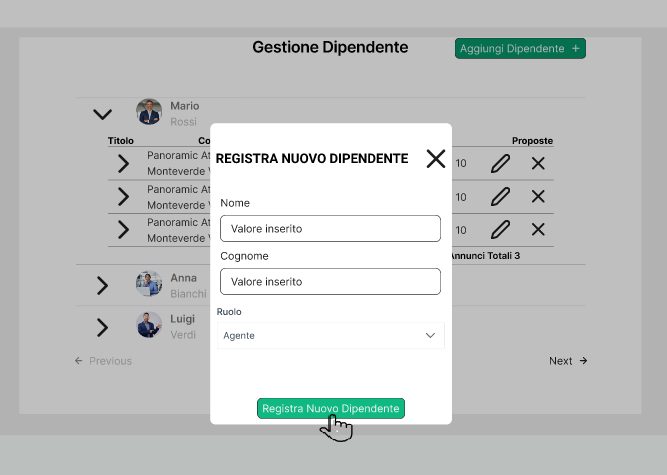
\includegraphics[width=0.7\textwidth]{Immagini/Mockup/nuovoAgente/scenario principale/clickFormNuovoAgente.png} \\
				Cockburn: step 2/3/4
			\end{tabular}
		};
		
		% Nodo per immagine 3 con didascalia sotto, posizionato sotto img2
		\node (img3) [below=of img2] {
			\begin{tabular}{c}
				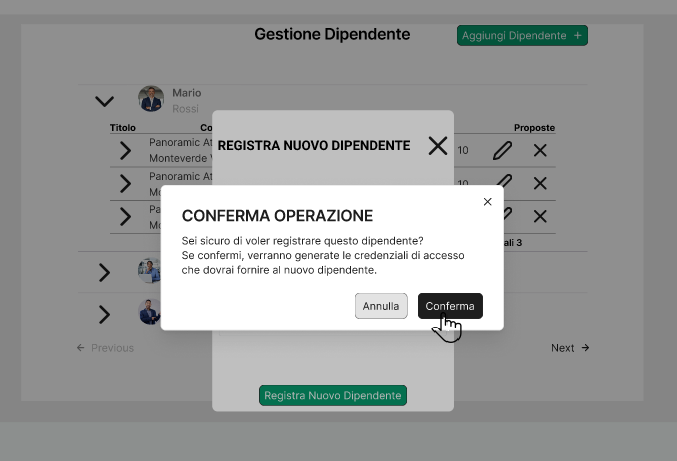
\includegraphics[width=0.7\textwidth]{Immagini/Mockup/nuovoAgente/scenario principale/ClickAllertConferma.png} \\
				Cockburn: step 5/6
			\end{tabular}
		};
		
		% Disegna le frecce
		\draw[->, thick] (img1) -- (img2);
		\draw[->, thick] (img2) -- (img3);
		
	\end{tikzpicture}
	\caption{Mockup: scenario principale della tabella di Cockburn del caso d'uso: Registra nuovo agente.}
	\label{fig:tikz_flow}
\end{figure}

\newpage

\begin{figure}[H]
	\centering
	\begin{tikzpicture}[node distance=1.5cm and 1cm, auto]
		% Nodo per immagine 1 con didascalia sotto
		\node (img1) {
			\begin{tabular}{c}
				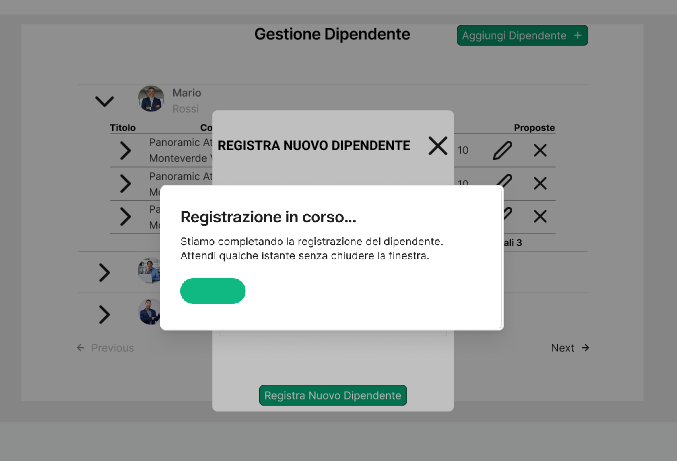
\includegraphics[width=0.7\textwidth]{Immagini/Mockup/nuovoAgente/scenario principale/caricamentoRegistrazione.png} \\
				Cockburn: step 6/7/9
			\end{tabular}
		};
		
		% Nodo per immagine 2 con didascalia sotto, posizionato a destra di img1
		\node (img2) [below=of img1] {
			\begin{tabular}{c}
				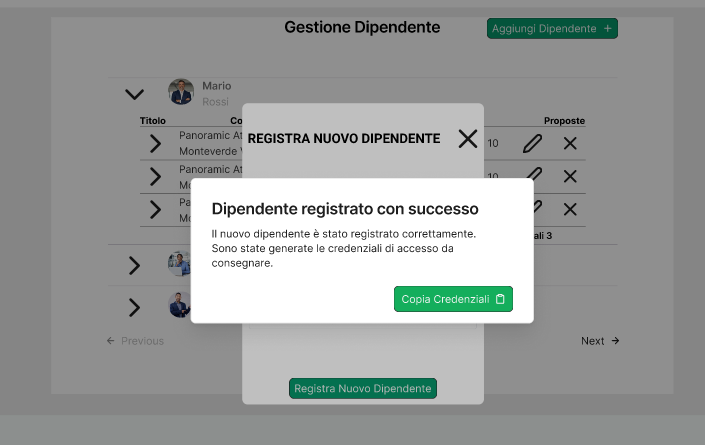
\includegraphics[width=0.7\textwidth]{Immagini/Mockup/nuovoAgente/scenario principale/allertRegistrazioneEffettuata.png} \\
				Cockburn: step 10
			\end{tabular}
		};
		
		% Nodo per immagine 3 con didascalia sotto, posizionato sotto img2
		\node (img3) [below=of img2] {
			\begin{tabular}{c}
				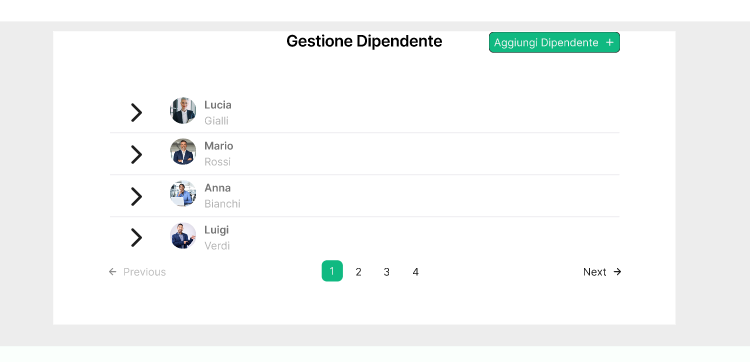
\includegraphics[width=0.7\textwidth]{Immagini/Mockup/nuovoAgente/scenario principale/visualizzazioneNuovaRegistrazione.png} \\
				Cockburn: step 11
			\end{tabular}
		};
		
		% Disegna le frecce
		\draw[->, thick] (img1) -- (img2);
		\draw[->, thick] (img2) -- (img3);
		
	\end{tikzpicture}
	\caption{Mockup: scenario principale della tabella di Cockburn del caso d'uso: Registra nuovo agente.}
	\label{fig:tikz_flow}
\end{figure}

\newpage

\input{Requisiti Del Software/Analisi dei Requisiti/Mockup/aggiungi nuovo agente/MockUp NuovoAgente extensions A}
\input{Requisiti Del Software/Analisi dei Requisiti/Mockup/aggiungi nuovo agente/MockUp NuovoAgente extensions B}
\input{Requisiti Del Software/Analisi dei Requisiti/Mockup/aggiungi nuovo agente/MockUp NuovoAgente extensions C}
\input{Requisiti Del Software/Analisi dei Requisiti/Mockup/aggiungi nuovo agente/MockUp NuovoAgente extensions D}


\clearpage
\newpage





% 3.Documento di Design del sistema
\chapter{Design del Sistema}
\section{Descrizione dell'architettura proposta}
L'architettura del nostro server è stata progettata per rispondere alle esigenze richieste dal cliente, dove è stata prioritizzata la velocità di sviluppo e deployment senza sacrificare robustezza e sicurezza. Abbiamo adottato un'architettura monolitica basata su una struttura a livelli, che facilita la separazione delle responsabilità e garantisce una maggiore manutenibilità nel tempo.

In particolare, il sistema è suddiviso nei seguenti strati:

\begin{itemize}
    \item Controllers: Responsabili della gestione delle richieste HTTP, questo livello si occupa di ricevere le chiamate dai client e di instradarle verso il livello successivo.
    \item Services: Qui risiede la logica di business. Il livello Service elabora le richieste provenienti dai Controllers, gestendo le regole e i processi applicativi.
    \item Repositories: Questo strato è dedicato alla persistenza dei dati, interagendo con il database attraverso l’uso di Hibernate e JPA per mappare le entità e gestire le operazioni di lettura/scrittura.

\end{itemize}
La scelta di un'architettura monolitica si giustifica con la necessità di ridurre la complessità iniziale e non rallentare lo sviluppo, mantenendo comunque una struttura modulare che potrà essere facilmente evoluta nel tempo – ad esempio, trasformando parti del sistema in microservizi qualora il progetto dovesse espandersi in futuro.

\newpage
\section{Descrizione e motivazione delle scelte tecnologiche adottate}
Le tecnologie selezionate per lo sviluppo del backend sono state scelte in base a una combinazione di familiarità e facilità d'uso, con l'obiettivo di accelerare il processo di implementazione e garantire al contempo solidità e qualità del codice. In particolare:

\begin{itemize}
    \item Java con Spring Boot: Abbiamo optato per questo framework grazie alle sue numerose configurazioni predefinite e utili estensioni come Lombok, che ci permettono di concentrarci sulla logica di business anziché su complesse configurazioni di sistema o codice ripetuto. Spring Boot consente di avviare rapidamente un'applicazione web robusta e scalabile.
    \item Hibernate: Per la gestione della persistenza, Hibernate si rivela una scelta efficace, in quanto astrae le operazioni di accesso al database e riduce significativamente il lavoro manuale nella scrittura di query SQL. Questo approccio rende il codice più leggibile e facilmente mantenibile.
    \item JWT (JSON Web Token): Per garantire un'autenticazione stateless e sicura, abbiamo deciso di utilizzare i JWT. Questa soluzione permette di gestire le sessioni degli utenti in maniera efficiente, differenziando eventuali ruoli o permessi e riducendo il carico sul server.
    \item Swagger: L’adozione di Swagger per la documentazione delle REST API agevola notevolmente il testing e la verifica degli endpoint, creando al contempo una documentazione ricca di informazioni utili per condividere informazioni critiche .
\end{itemize}

 
\section{Descrizione dello schema per la persistenza dati}
La gestione della persistenza dei dati è centrale per il nostro backend e si basa su un modello che sfrutta le potenzialità di Hibernate.  PostgreSQL, per la loro affidabilità e diffusione nell’ecosistema Java.

Hibernate si occupa di:

Mappare le entità: Le classi Java rappresentano le entità del dominio, le quali vengono automaticamente correlate alle tabelle del database.
Gestire le relazioni: Le associazioni fra le entità (uno-a-uno, uno-a-molti, molti-a-molti) sono gestite in modo trasparente, riducendo la complessità nella scrittura delle query.
Ottimizzare le operazioni di lettura e scrittura: Grazie al supporto per caching e gestione delle transazioni, Hibernate semplifica l’interazione con il DBMS e contribuisce a mantenere il sistema performante e affidabile.
\newpage
\begin{figure}
    \centering
    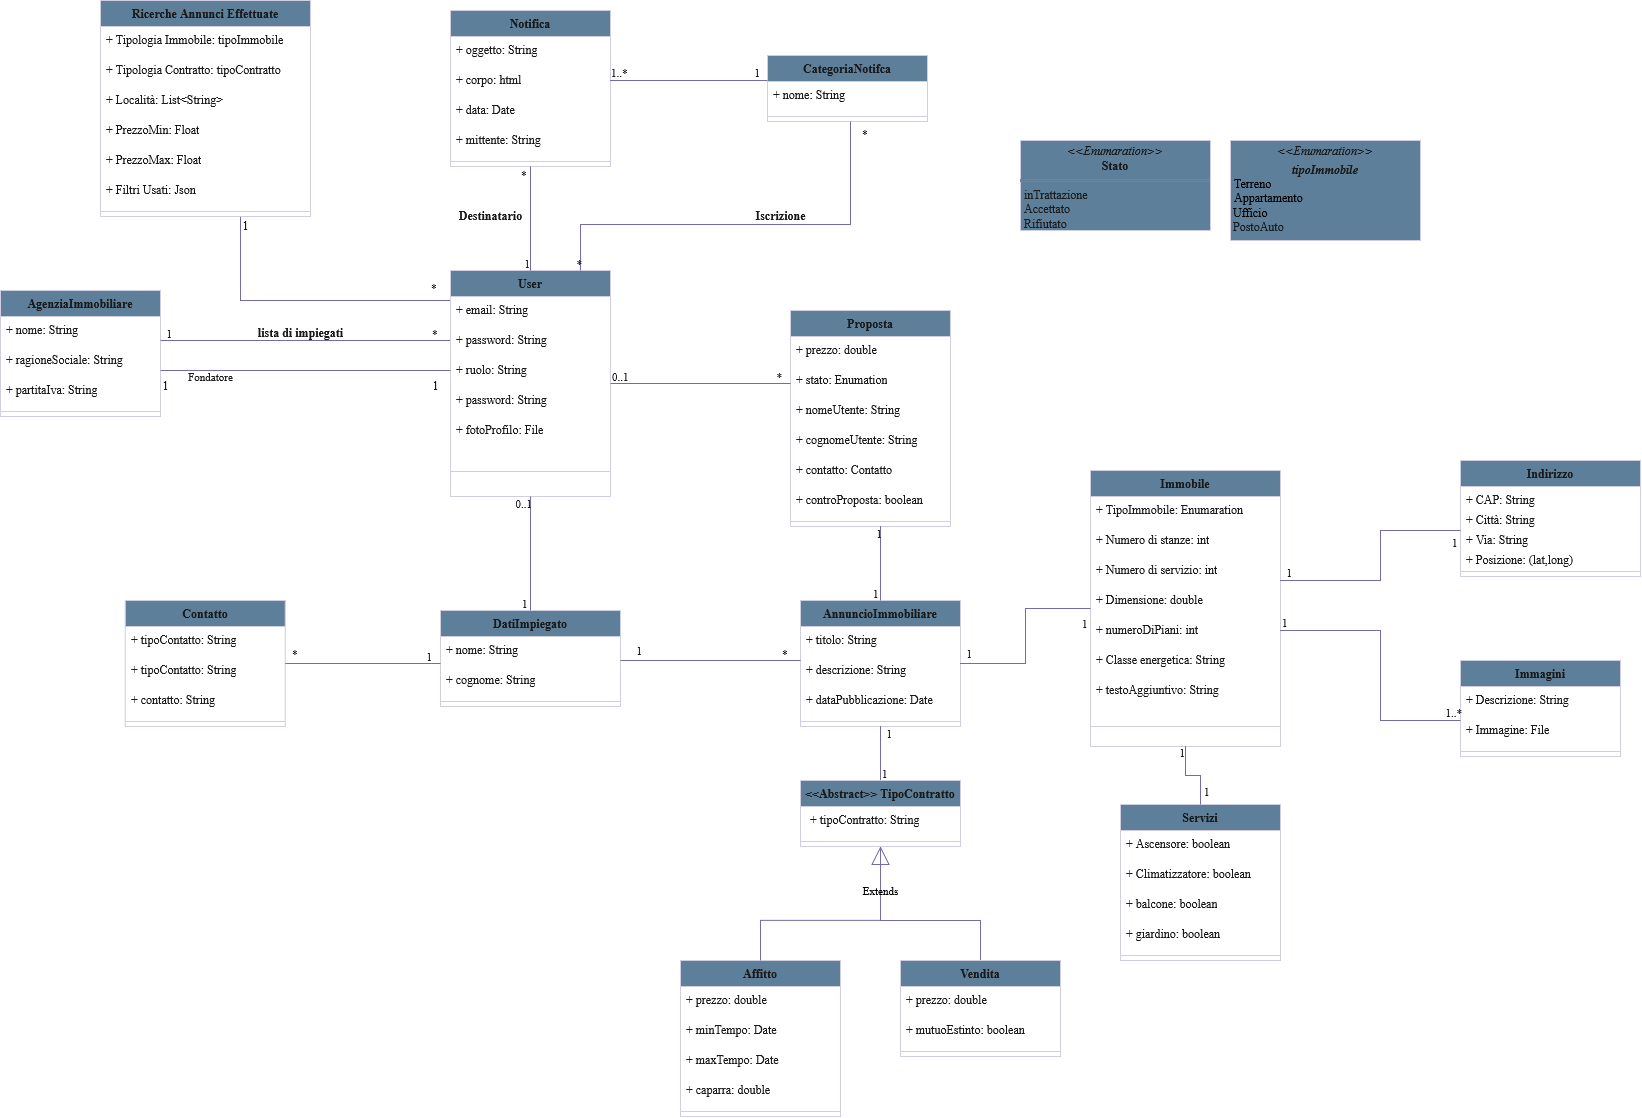
\includegraphics[width=1
    \linewidth]{Immagini/diagramma delle classi.drawio.png}
    \caption{Diagramma delle classi usate}
    \label{fig:enter-label}
\end{figure}

\section{Descrizione e motivazioni delle tecnologie adottate }
In questa sezione vengono presentate le tecnologie adottate per l’implementazione delle componenti client e server del sistema.
Inoltre, vengono descritte le architetture specifiche utilizzate nel back-end, in relazione alle tecnologie impiegate, e quelle adottate nel front-end.

\subsection{Tecnologie e architettura beckend}
L'architettura del nostro server è stata progettata per rispondere alle esigenze richieste dal cliente, dove è stata prioritizzata la velocità di sviluppo e deployment senza sacrificare robustezza e sicurezza. Abbiamo adottato un'architettura \textbf{monolitica} basata su una struttura a livelli, che facilita la separazione delle responsabilità e garantisce una maggiore manutenibilità nel tempo. La scelta di un'architettura monolitica si giustifica con la necessità di ridurre la complessità iniziale e non rallentare lo sviluppo, mantenendo comunque una struttura modulare che potrà essere facilmente evoluta nel tempo, ad esempio, trasformando parti del sistema in microservizi qualora il progetto dovesse espandersi in futuro.
\\
Le tecnologie selezionate per lo sviluppo del backend sono state scelte in base a una combinazione di familiarità e facilità d'uso, con l'obiettivo di accelerare il processo di implementazione e garantire al contempo solidità e qualità del codice.
\\
Il back-end è stato sviluppato utilizzando \textbf{Spring Boot}, abbiamo optato per questo framework grazie alle sue numerose configurazioni predefinite e utili estensioni come \textbf{Lombok}, che ci permettono di concentrarci sulla logica di business anziché su complesse configurazioni di sistema o codice ripetuto. Spring Boot consente di avviare rapidamente un'applicazione web robusta e scalabile.
esso sono state integrate diverse tecnologie complementari, tra cui:

\begin{itemize}
	\item \textbf{Hibernate}: Per la gestione della persistenza, Hibernate si rivela una scelta efficace, in quanto astrae le operazioni di accesso al database e riduce significativamente il lavoro manuale nella scrittura di query SQL. Questo approccio rende il codice più leggibile e facilmente mantenibile.
	
	\item \textbf{Spring Security e JWT (JSON Web Token)}: Per garantire un'autenticazione stateless e sicura, abbiamo deciso di utilizzare i JWT. Questa soluzione permette di gestire le sessioni degli utenti in maniera efficiente, differenziando eventuali ruoli o permessi e riducendo il carico sul server.
	
	\item \textbf{Jackson}: È uno strumento potente per serializzare e deserializzare oggetti Java in \textbf{JSON} e viceversa.
	Quando si utilizza l’annotazione \colorbox{lightgray}{@RestController} o \colorbox{lightgray}{@ResponseBody}, Spring Boot restituisce automaticamente le risposte in formato JSON senza necessità di configurazioni aggiuntive.
	
	\item \textbf{Swagger}: L’adozione di Swagger per la documentazione delle REST API agevola notevolmente il testing e la verifica degli endpoint, creando al contempo una documentazione ricca di informazioni utili per condividere informazioni critiche.
\end{itemize}

Il back-end del sistema segue il pattern architetturale \textbf{MVC (Model-View-Controller)}, nativamente supportato dal framework \textbf{Spring Boot}.
Nel nostro caso, il \textbf{Model} è rappresentato dalle entità e dalla logica di business implementata nei servizi; il \textbf{Controller} è costituito dai componenti RESTful che gestiscono e mappano le richieste HTTP.
La \textbf{View} non è gestita all’interno del back-end, poiché l’applicazione svolge il ruolo di \textbf{API REST}, restituendo risposte in formato JSON al client, che si occupa della rappresentazione dei dati.
Questo approccio garantisce una chiara \textbf{separazione delle responsabilità}, migliorando la \textbf{modularità} e la \textbf{manutenibilità} del sistema.
\\ \\
Di seguito viene riportato uno schema del design utilizzato del backend

\begin{figure}[H]
	\centering
	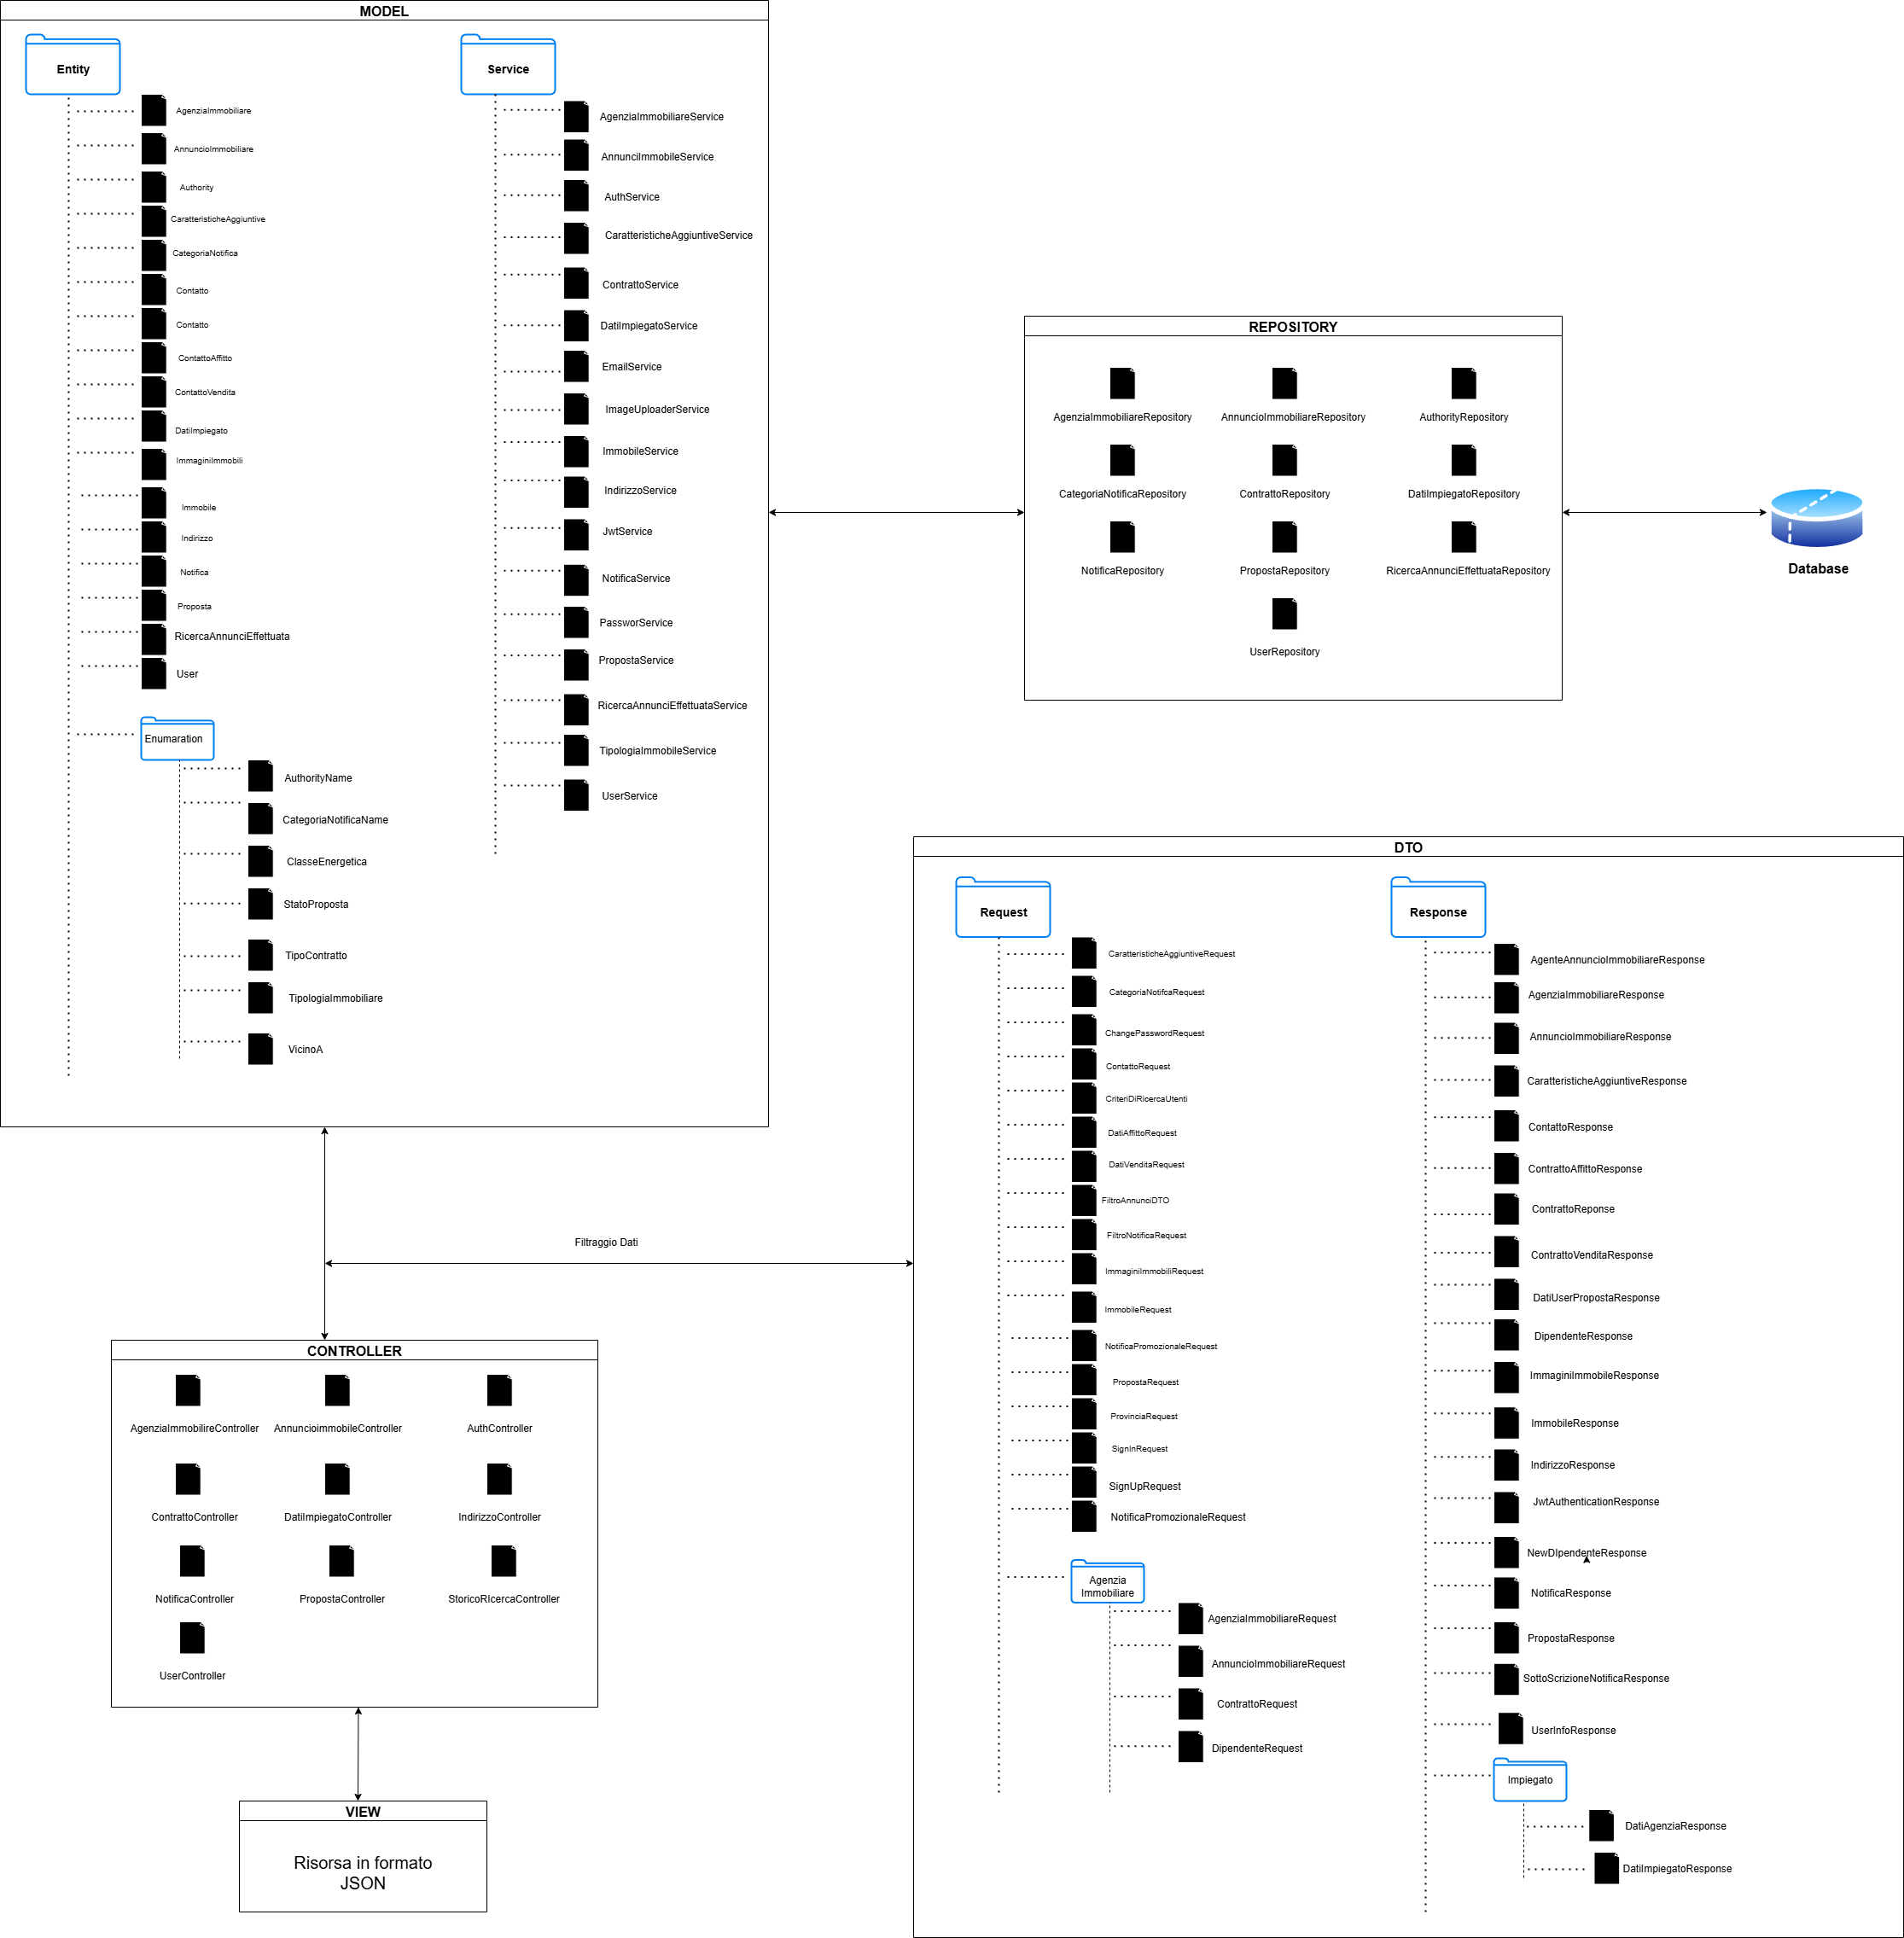
\includegraphics[width=0.7\linewidth]{Immagini/Schema backend.png}
	\caption[schema backend]{Schema sintetico dell'architettura del backend}
\end{figure}

\section{Descrizione dello schema per la persistenza dati}
La gestione della persistenza dei dati è centrale per il nostro backend e si basa su un modello che sfrutta le potenzialità di Hibernate.  PostgreSQL, per la loro affidabilità e diffusione nell’ecosistema Java.

Hibernate si occupa di:

Mappare le entità: Le classi Java rappresentano le entità del dominio, le quali vengono automaticamente correlate alle tabelle del database.
Gestire le relazioni: Le associazioni fra le entità (uno-a-uno, uno-a-molti, molti-a-molti) sono gestite in modo trasparente, riducendo la complessità nella scrittura delle query.
Ottimizzare le operazioni di lettura e scrittura: Grazie al supporto per caching e gestione delle transazioni, Hibernate semplifica l’interazione con il DBMS e contribuisce a mantenere il sistema performante e affidabile.
\newpage
\begin{figure}
	\centering
	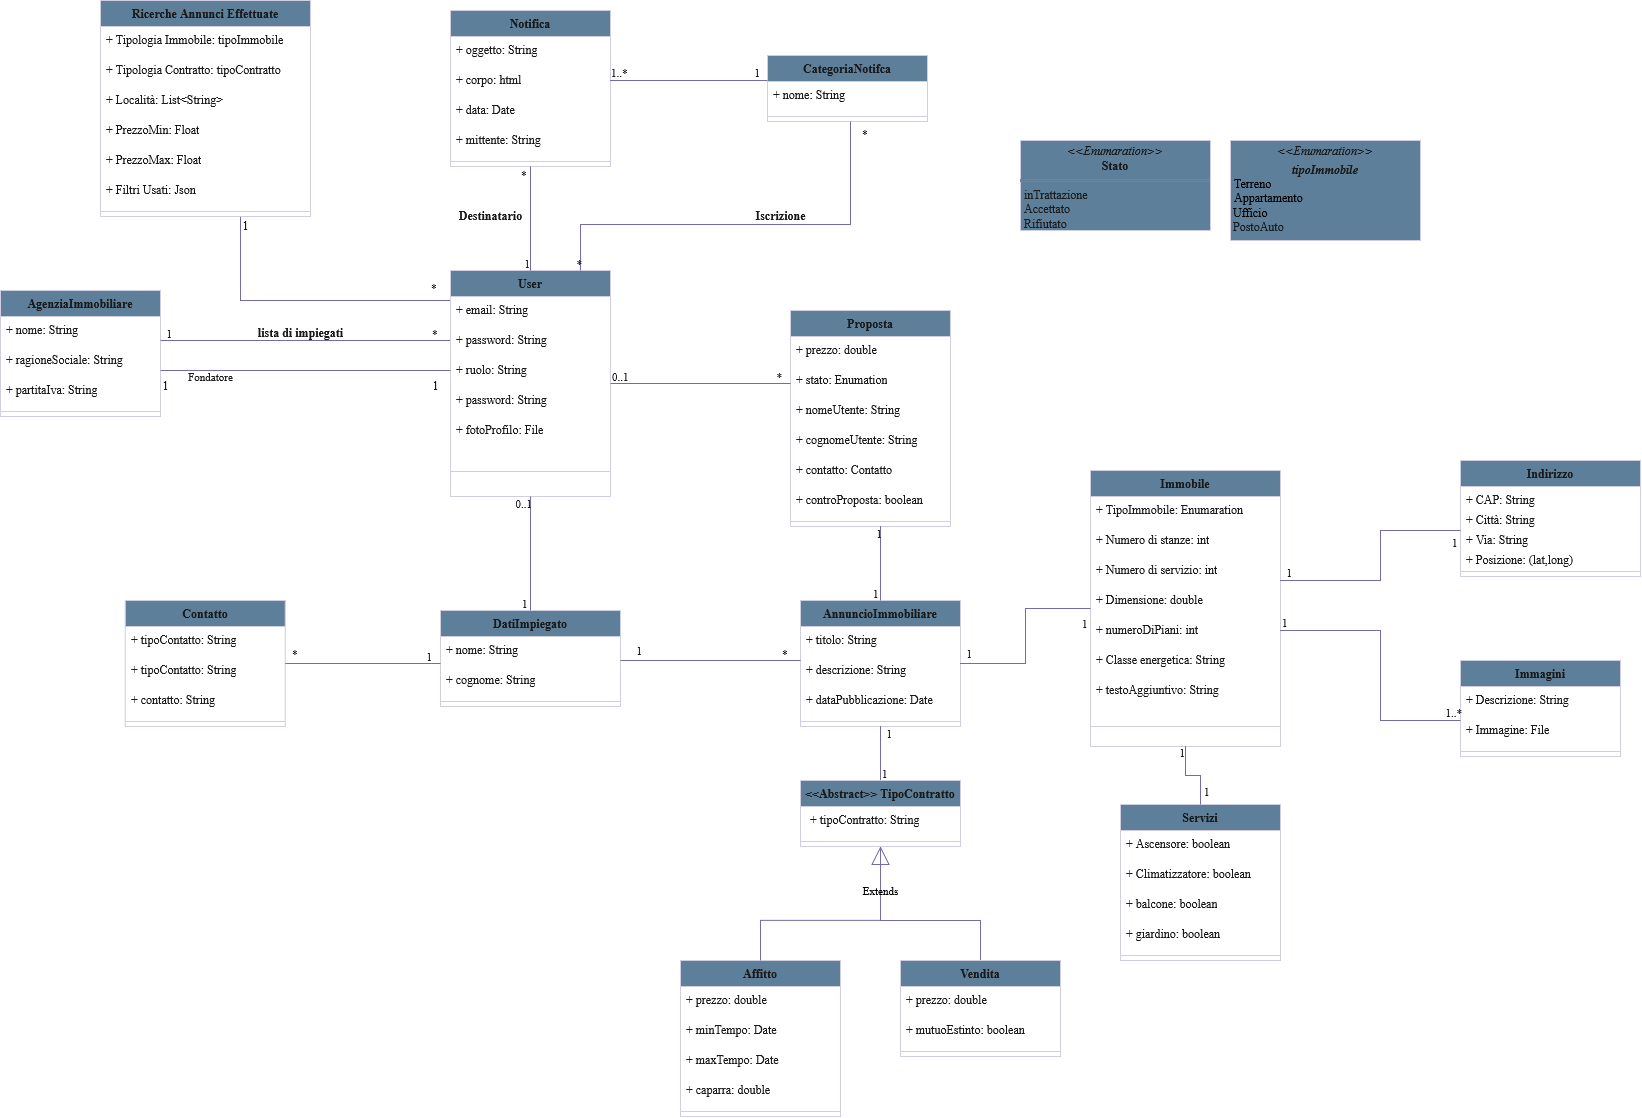
\includegraphics[width=1
	\linewidth]{Immagini/diagramma delle classi.drawio.png}
	\caption{Diagramma delle classi usate}
	\label{fig:enter-label}
\end{figure}

\input{Design del Sistema/Diagramma delle classi di design}
\section{Sequence diagram}

\subsection{Caso d'uso: Aggiungi un Annuncio Immobiliare}

\begin{figure}[H]
	\centering
	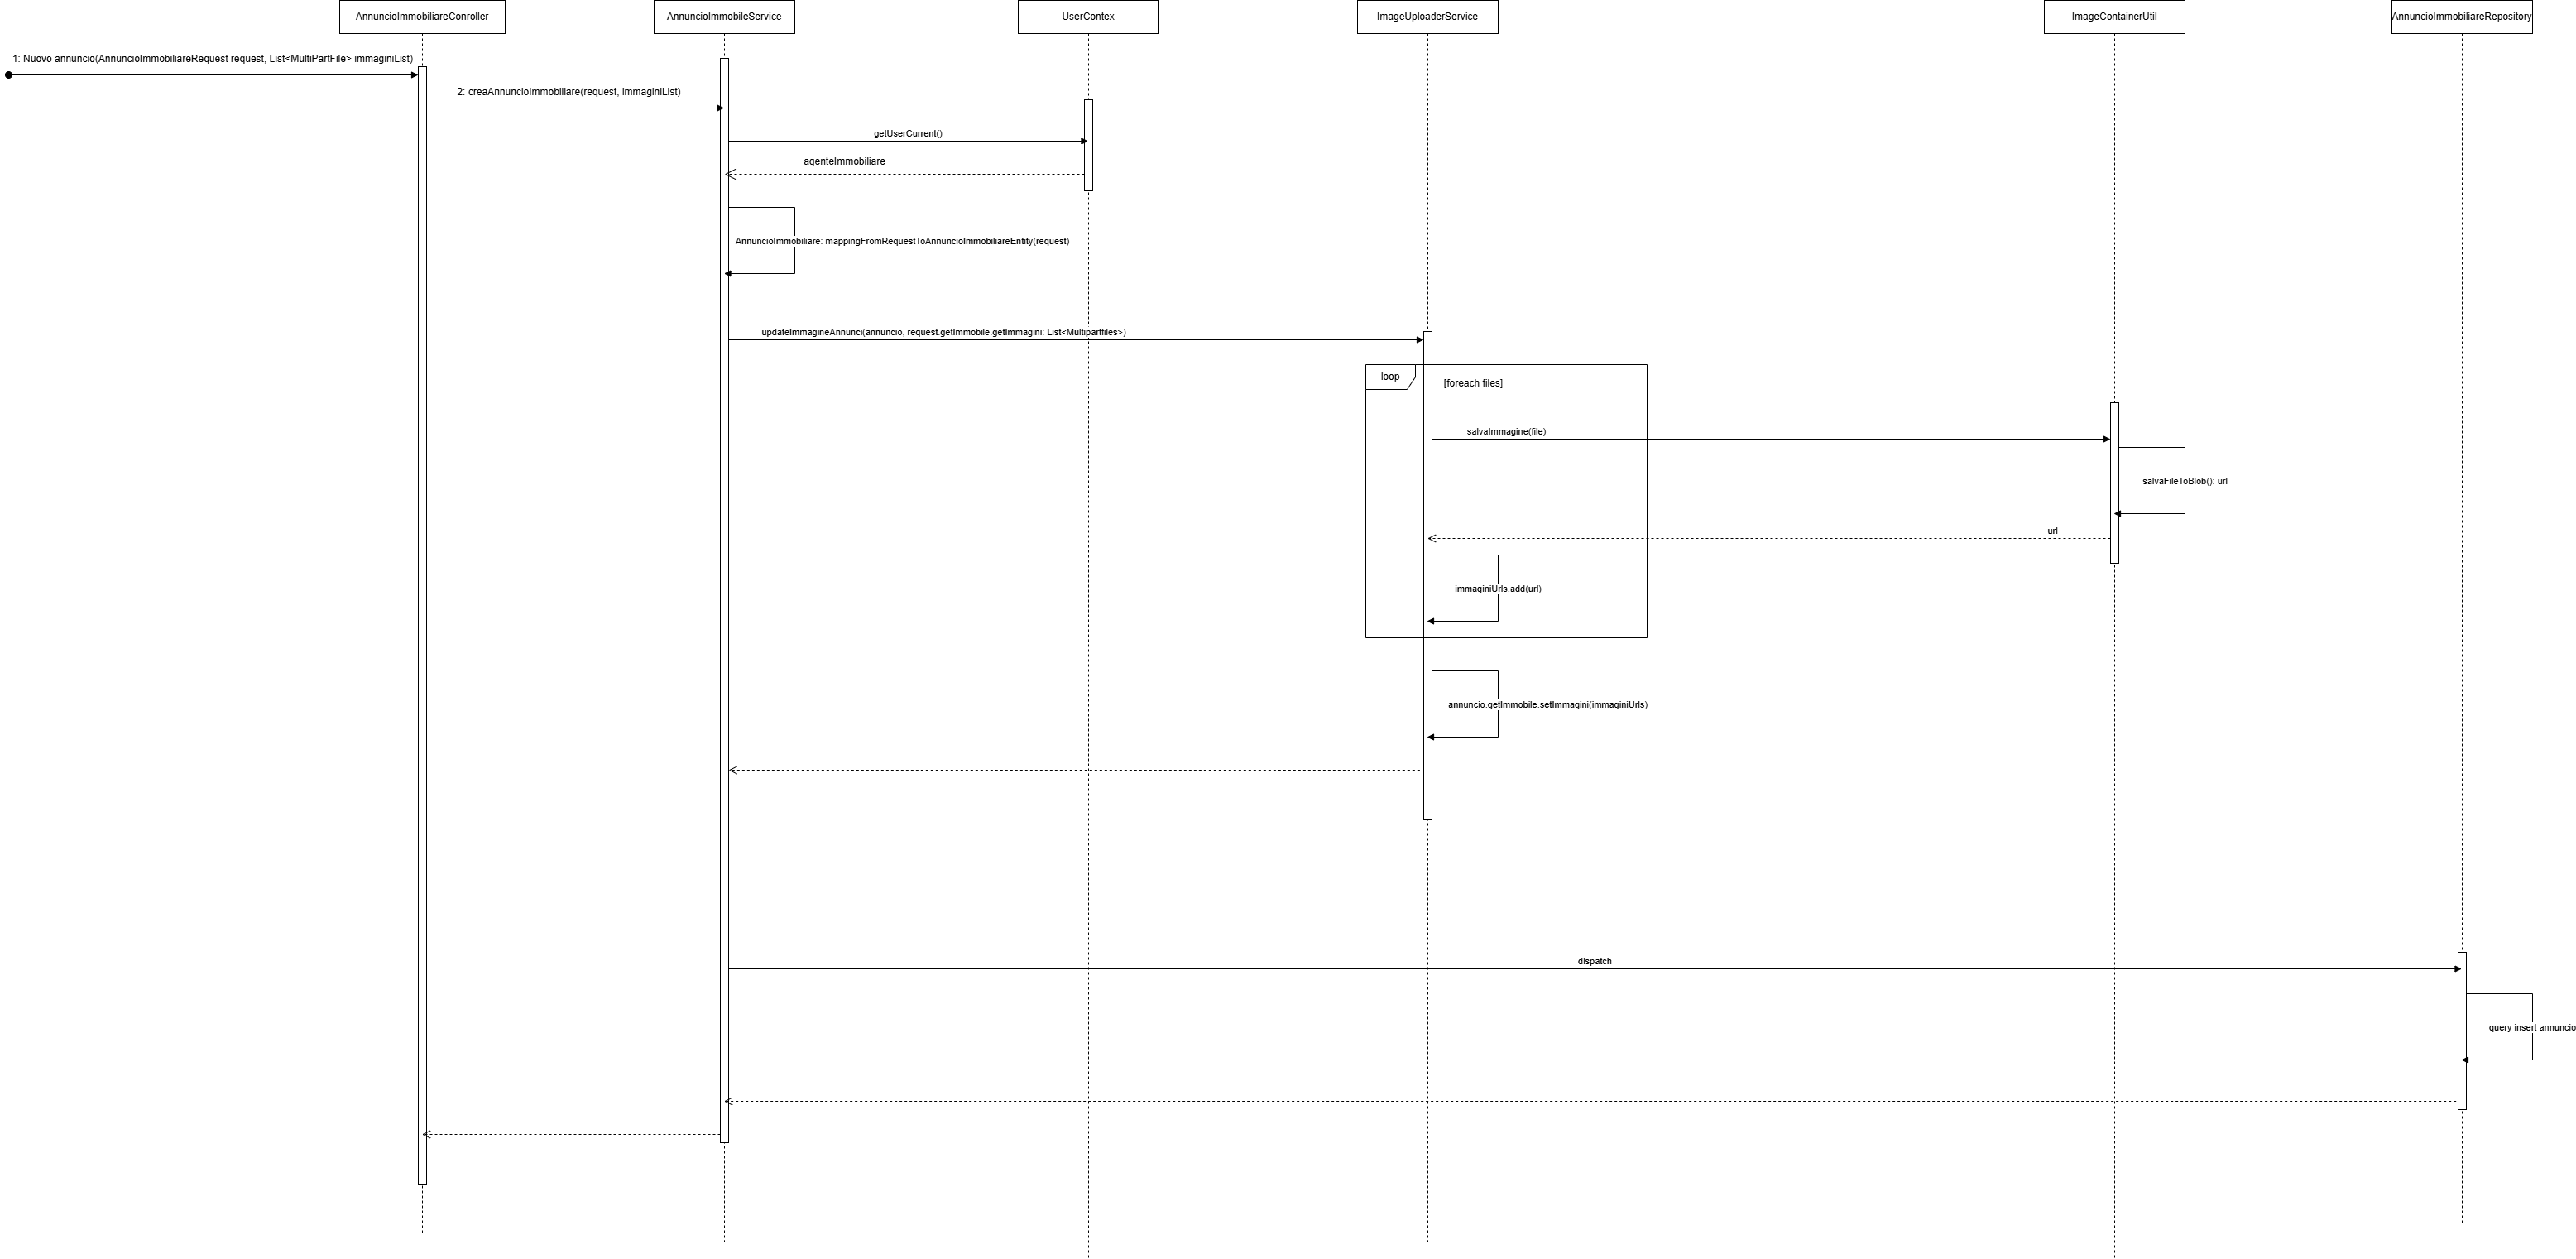
\includegraphics[width=\textwidth,height=\textheight,keepaspectratio]{Immagini/Sequence diagram/SequenceDiagram inserimentoAnnuncio.png}
	\caption[Sequence diagram 1]{Sequence Diagram del caso d'uso: Inserimento annuncio immobiliare}
\end{figure}

\subsection{Caso d'uso: Attivazione e Disattivazione Notifiche}

\begin{figure}[H]
	\centering
	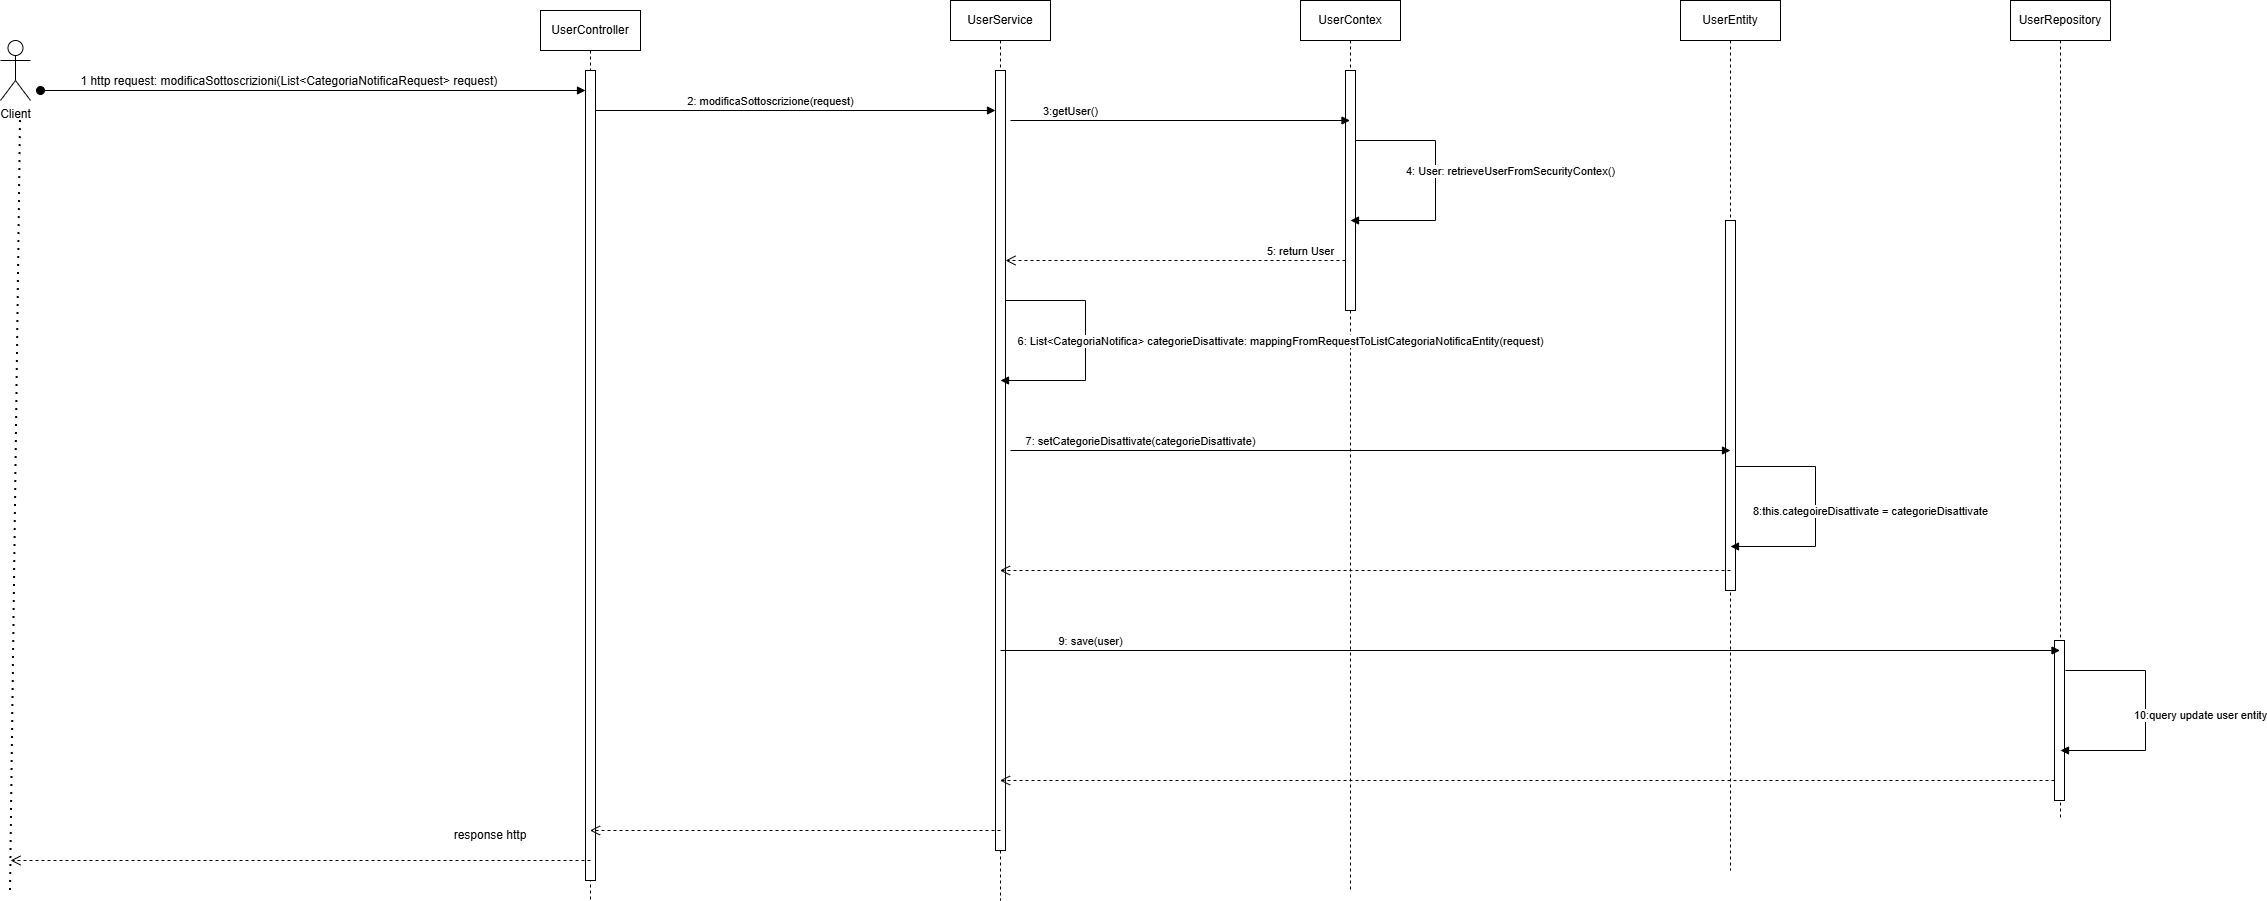
\includegraphics[width=\textwidth,height=\textheight,keepaspectratio]{Immagini/Sequence diagram/Sequence Diagram Gestione Notifiche.png}
	\caption[Sequence diagram 2]{Sequence Diagram del caso d'uso: Attivazione e Disattivazione Notifiche}
\end{figure}

\subsection{Caso d'uso: Controproposta di un'offerta}

\begin{figure}[H]
	\centering
	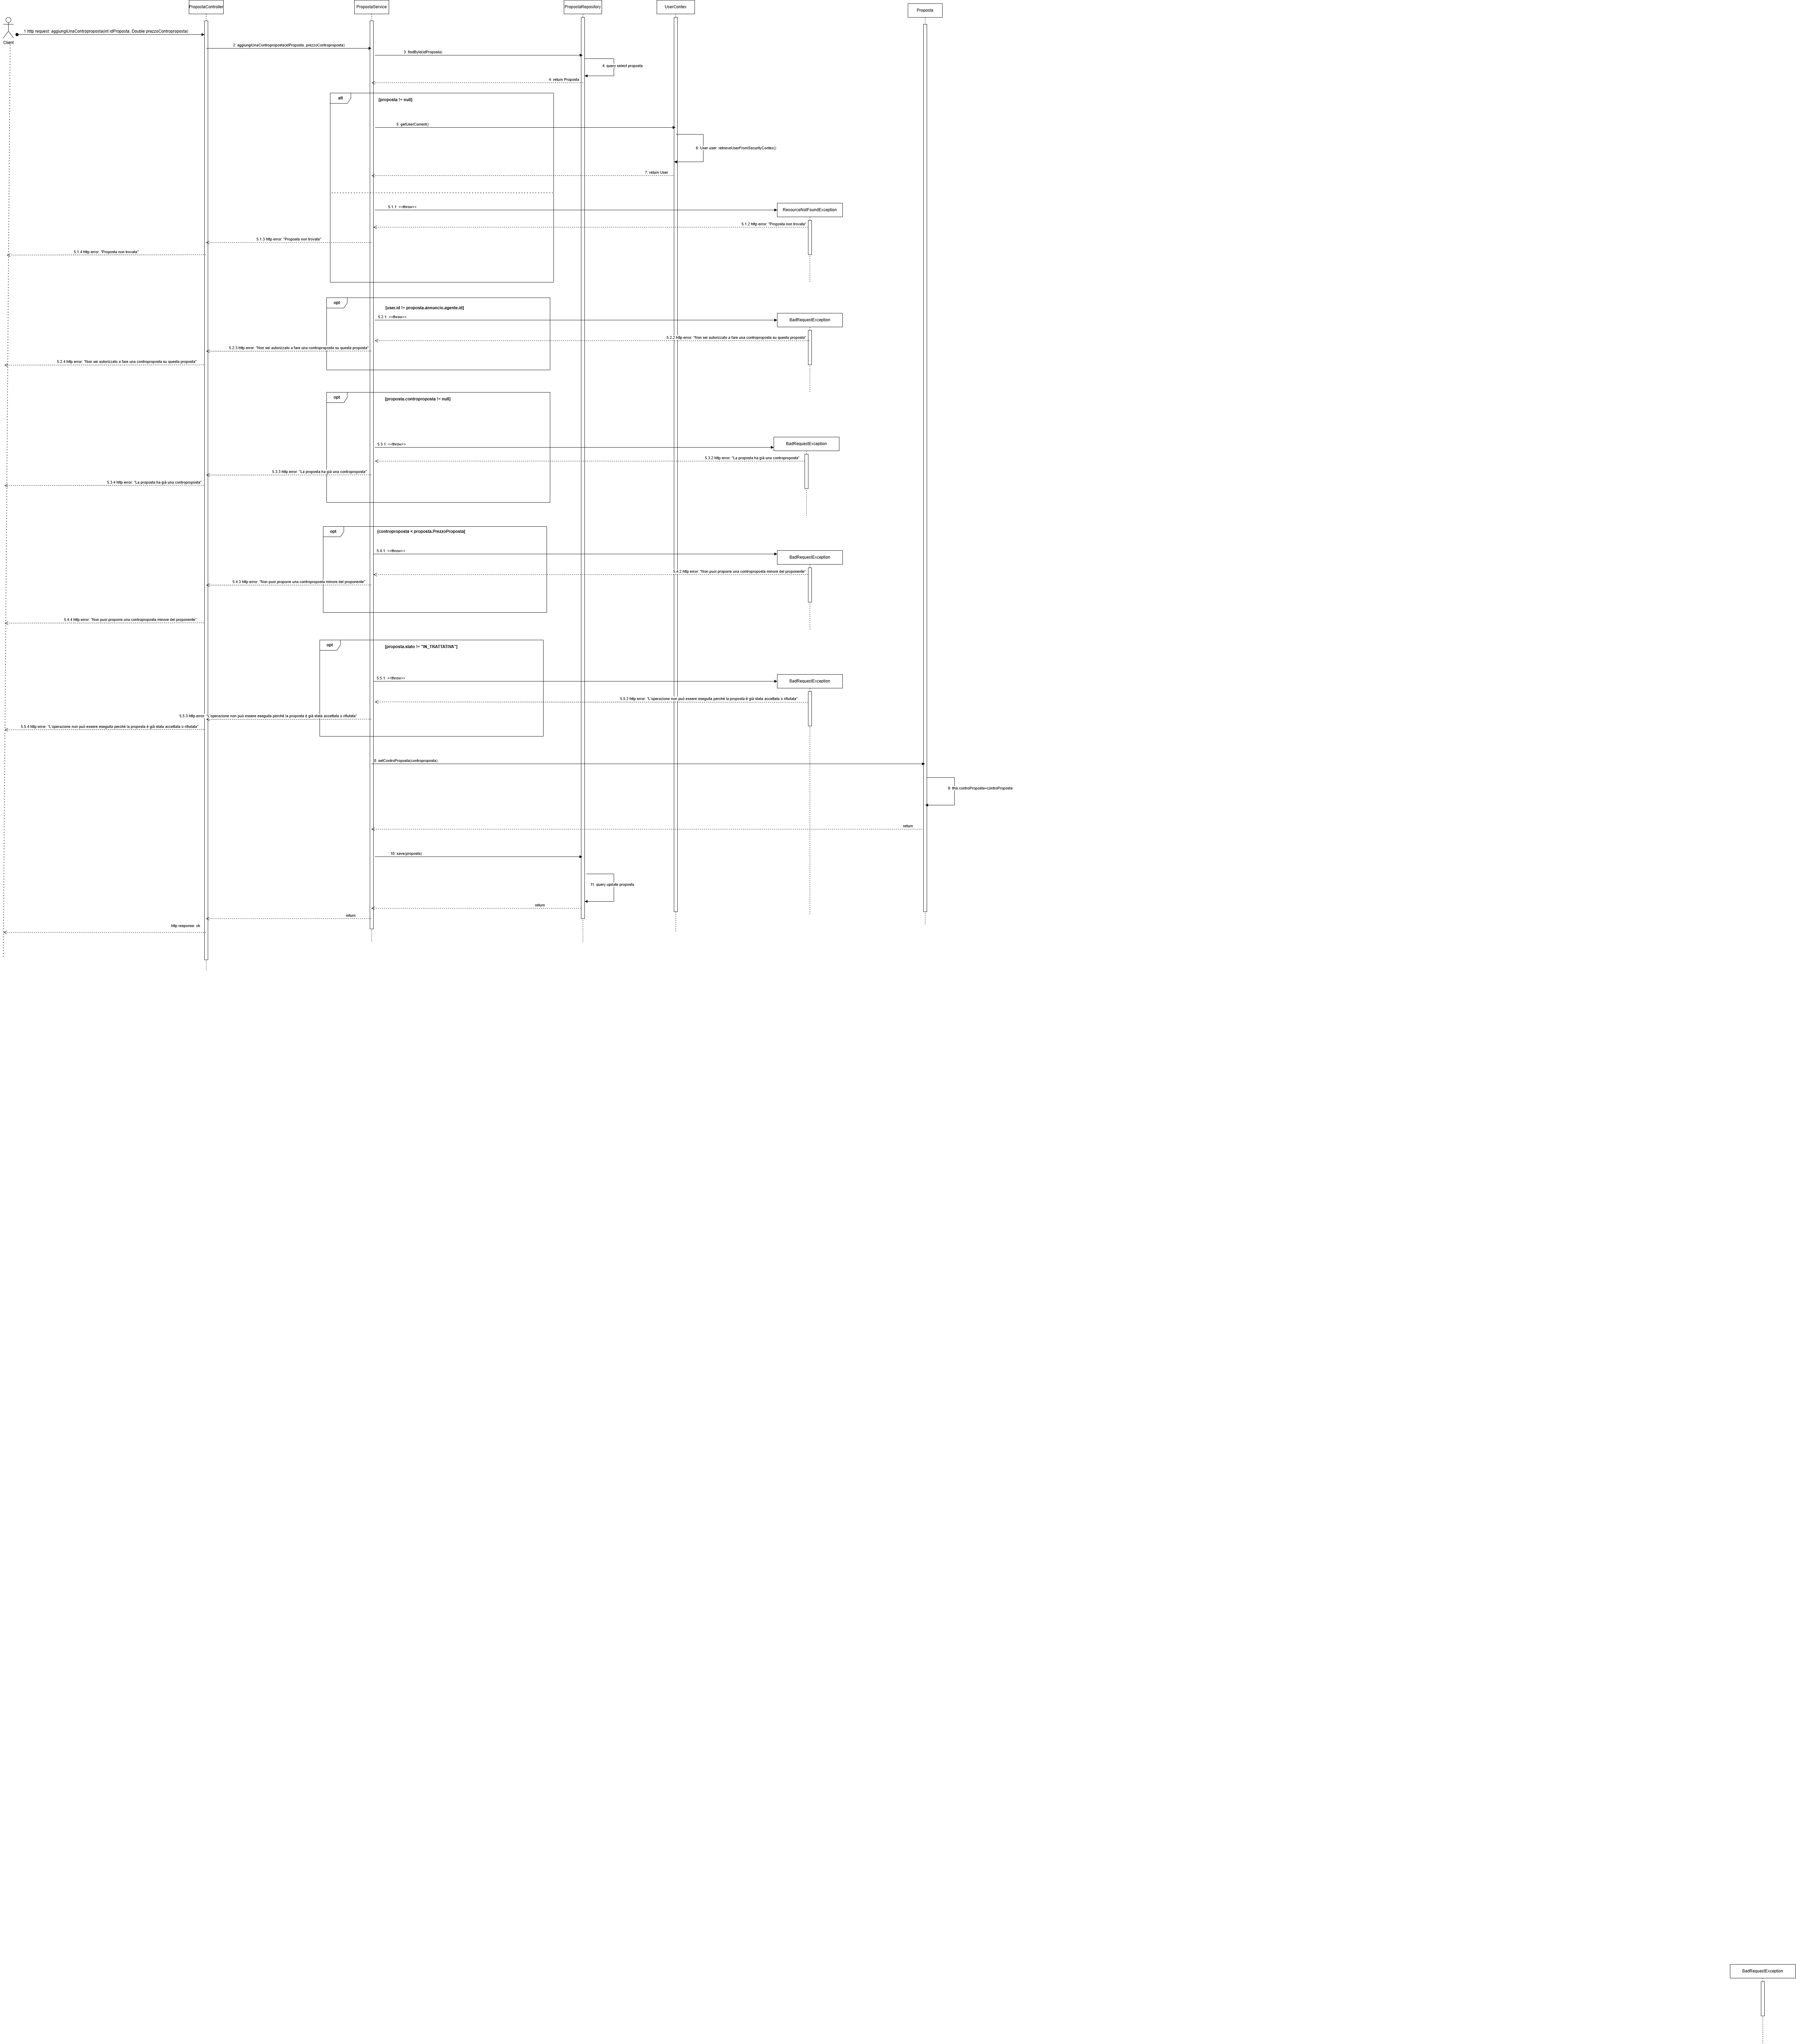
\includegraphics[width=\textwidth,height=\textheight,keepaspectratio]{Immagini/Sequence diagram/Sequence Diagram Effettua Controproposta.png}
	\caption[Sequence diagram 3]{Sequence Diagram del caso d'uso: Controproposta di un'offerta}
\end{figure}

\subsection{Caso d'uso: Registrazione di un Nuovo Agente}

\begin{figure}[H]
	\centering
	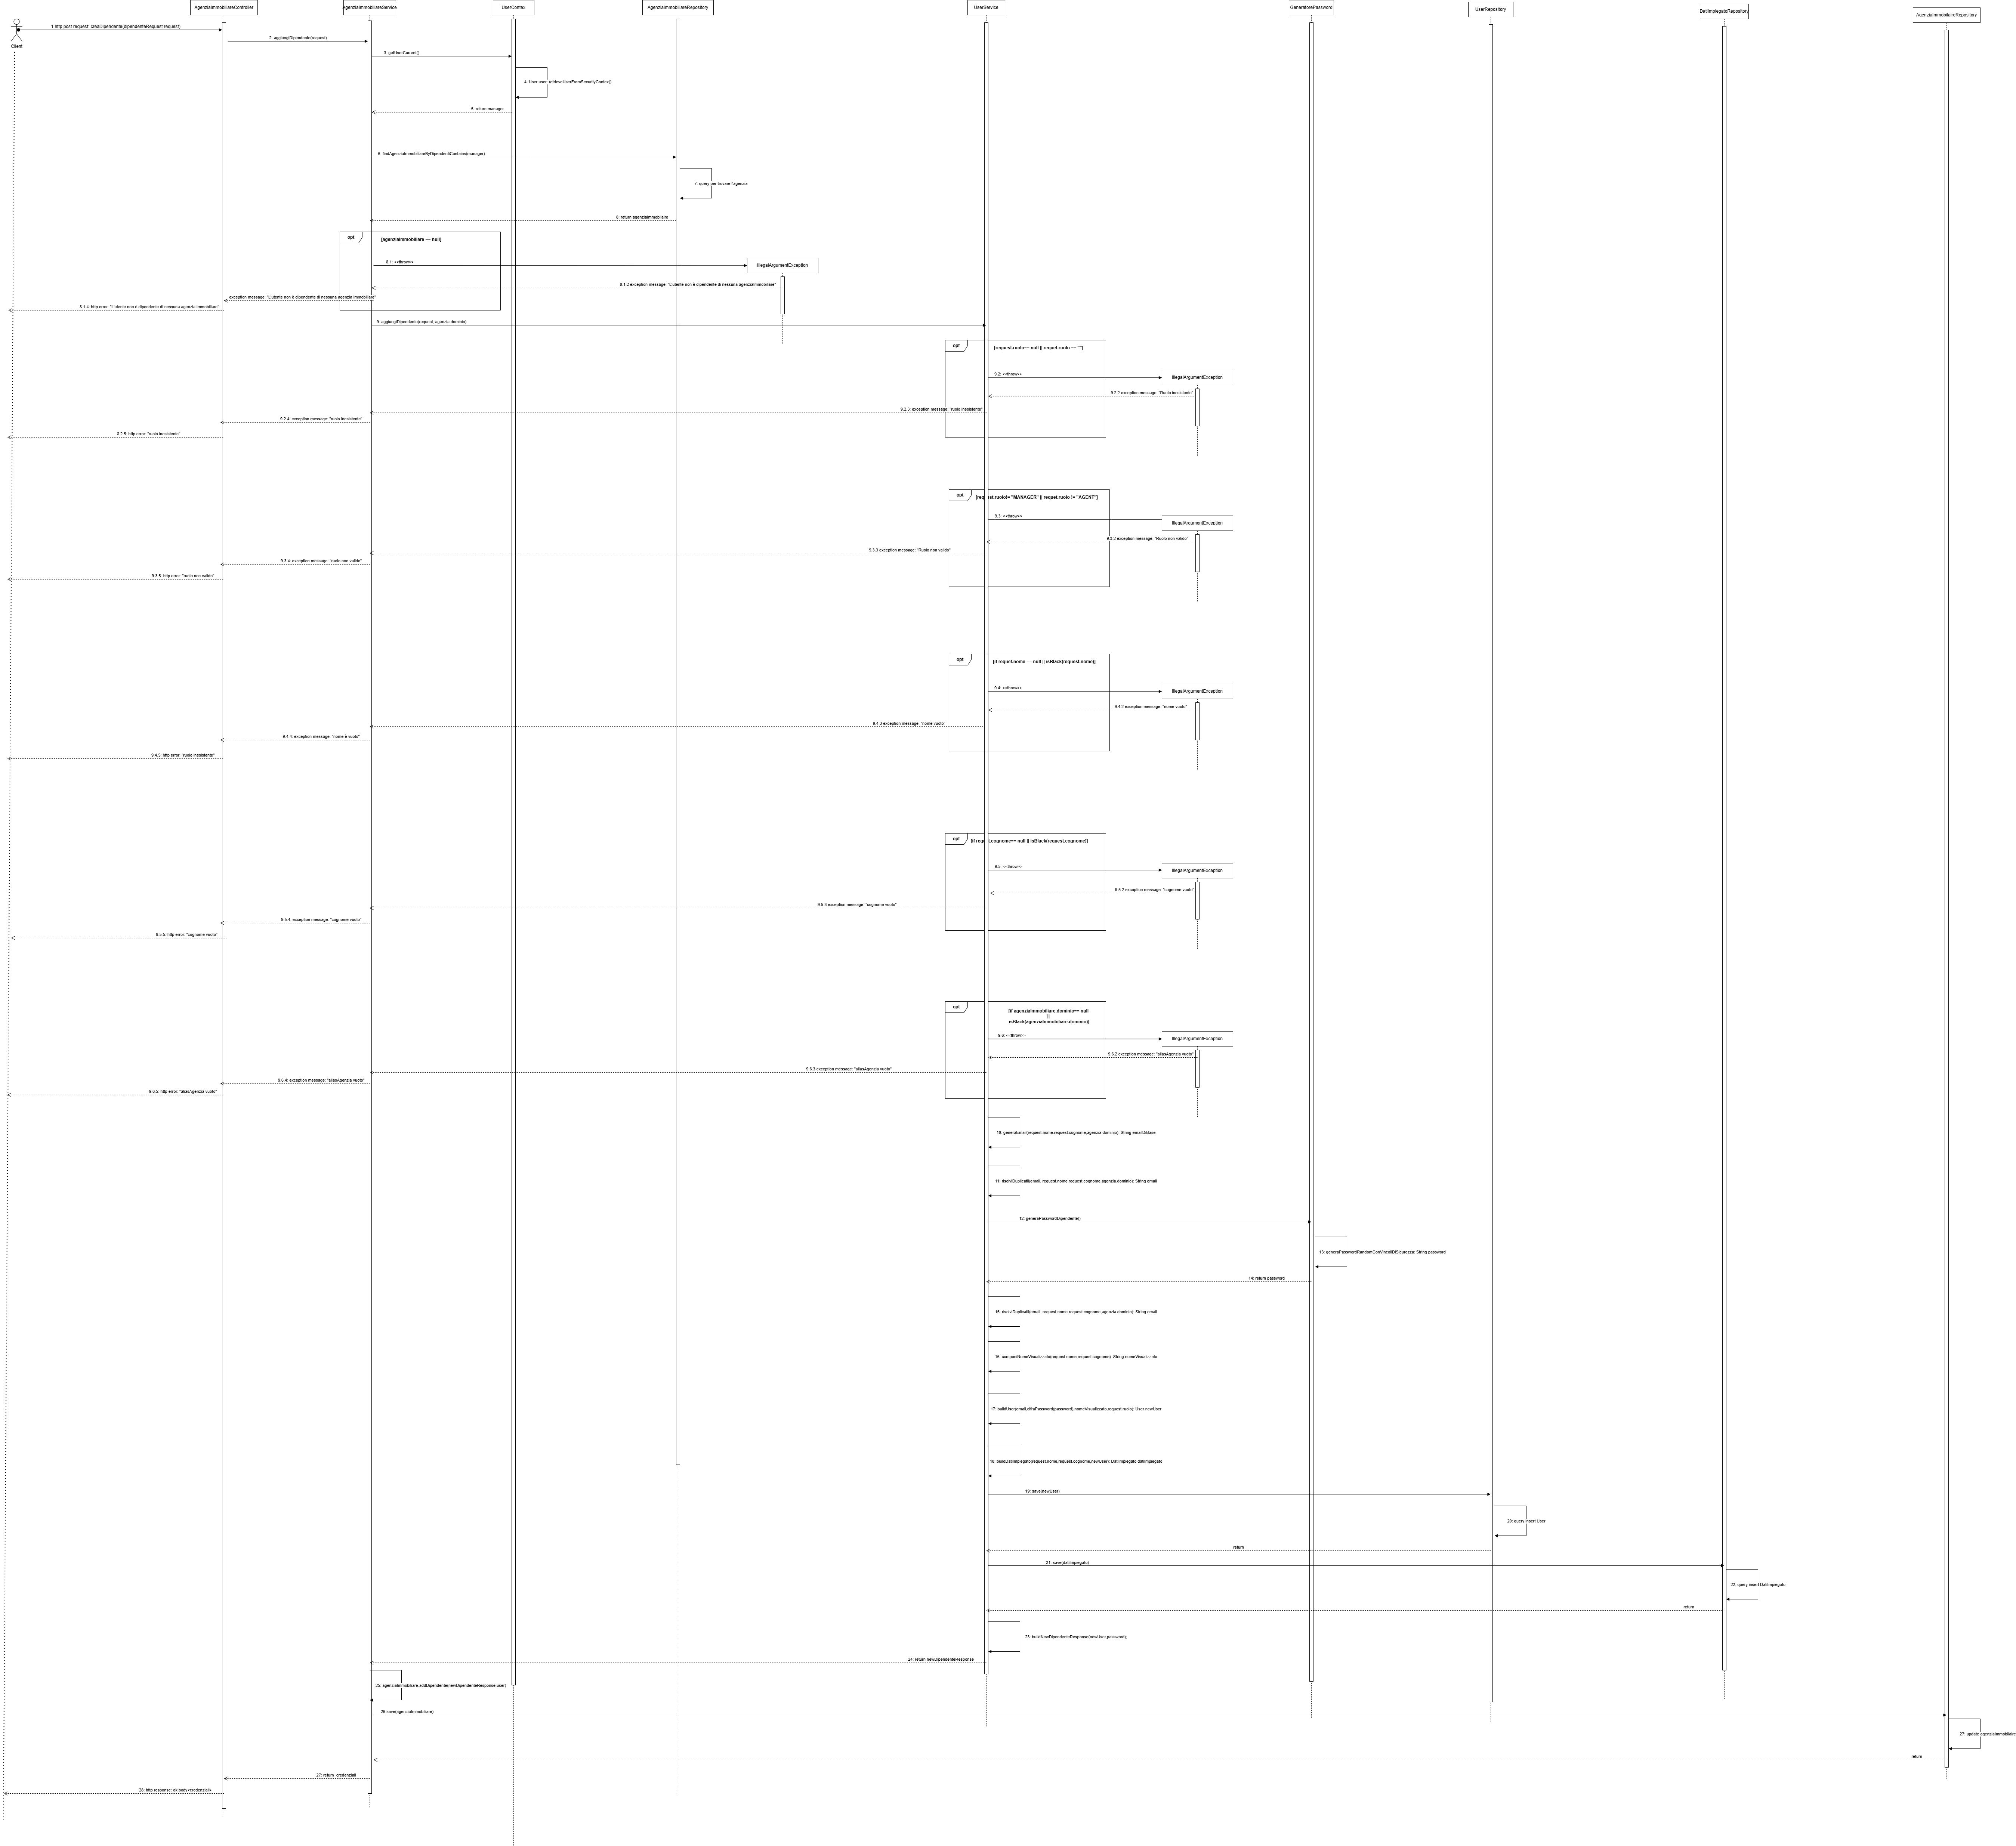
\includegraphics[width=\textwidth,height=\textheight,keepaspectratio]{Immagini/Sequence diagram/Sequence Diagram Aggiungi Dipendente.png}
	\caption[Sequence diagram 4]{Sequence Diagram del caso d'uso: Aggiungi Dipendente}
\end{figure}



% 4.Artefatti Software e documentazione del processo di sviluppo
\chapter{Processo di sviluppo}
\section{Introduzione}
Quando si sviluppa un software complesso, diventa necessario pianificare il lavoro da svolgere per creare un prodotto robusto e affidabile.\\
In questa sezione discuteremo dei metodi utilizzati per migliorare lo sviluppo del software, come il sistema di versionamento utilizzato e gli strumenti di pulizia del codice usati per ottenere un prodotto di alta qualità.\\
\section{Versionamento del codice}
È deciso di adottare il sistema di versionamento Git, usando la piattaforma GitHub per ospitare il repository del progetto. Essendo l'applicazione divisa in due blocchi precisi e distinti, il Front end Vue e il Server Backend Spring Boot, sono stati creati due repository per gestirli in modo separato ed evitare maggiori conflitti durante lo sviluppo.\\


% 5.Testing e valutazione dell’usabilità.
\chapter{Testing unitari}
\section{Introduzione}
Quando si sviluppa un software complesso, diventa necessario pianificare il lavoro da svolgere per creare un prodotto robusto e affidabile.\\
In questa sezione discuteremo dei metodi utilizzati per migliorare lo sviluppo del software, come il sistema di versionamento utilizzato e gli strumenti di pulizia del codice usati per ottenere un prodotto di alta qualità.\\
\section{Versionamento del codice}
È deciso di adottare il sistema di versionamento Git, usando la piattaforma GitHub per ospitare il repository del progetto. Essendo l'applicazione divisa in due blocchi precisi e distinti, il Front end Vue e il Server Backend Spring Boot, sono stati creati due repository per gestirli in modo separato ed evitare maggiori conflitti durante lo sviluppo.\\


% 6.Valutazione dell’usabilità.
\chapter{Valutazione dell'usabilità}
La \textbf{valutazione dell'usabilità} rappresenta una fase essenziale nel processo di sviluppo di un’interfaccia utente, consentendo di valutare l'efficacia, l’efficienza e la soddisfazione dell’utente nell’interazione con il sistema. In particolare, l'uso di mockup interattivi offre la possibilità di raccogliere feedback sulle scelte di design prima ancora della fase di sviluppo, riducendo i costi di eventuali revisioni e migliorando la qualità dell’esperienza utente.
\newline
L'obiettivo principale di questa sezione è identificare eventuali problemi di navigazione, ambiguità nelle interazioni o difficoltà nella comprensione delle funzionalità, al fine di ottimizzare l'interfaccia prima del rilascio definitivo.

\section{Expert Reviews / Inspections}

Per valutare la qualità complessiva dell’esperienza utente e la coerenza progettuale del sistema, è stata pianificata una revisione sistematica dell’interfaccia basata su una \textbf{valutazione euristica} secondo i principi di Nielsen \cite{nielsen1995}.  
L’attività ha avuto l’obiettivo di identificare punti di forza, criticità e incoerenze nel design, analizzando in due fasi distinte il \textit{prototipo realizzato in Figma} e successivamente la \textit{versione web implementata}.  

La revisione del prototipo Figma ha rappresentato un passaggio fondamentale prima dello sviluppo effettivo: ha consentito di riflettere in modo critico sulle scelte di interfaccia, di validare le principali logiche di navigazione e di anticipare eventuali problemi di usabilità.  
A differenza della versione web, il prototipo non consente un’interazione reale, ma offre comunque una base solida per verificare la chiarezza dei flussi e la coerenza visiva complessiva.

\subsection*{Obiettivi della Review}

Gli obiettivi principali dell’attività di \textit{Expert Review} sono stati:
\begin{itemize}
    \item Valutare la \textbf{usabilità} dei flussi principali del sistema, verificando la chiarezza dei percorsi e delle azioni disponibili.
    \item Analizzare la \textbf{coerenza visiva} rispetto alle linee guida di design definite nel brand e nel prototipo.
    \item Individuare problemi di \textbf{chiarezza, navigabilità e feedback} che possano compromettere l’esperienza d’uso.
    \item Identificare eventuali mancanze o ridondanze, con l’obiettivo di \textbf{migliorare la struttura informativa e la consistenza visiva}.
    \item Definire raccomandazioni per le fasi successive di sviluppo, in vista della revisione della \textbf{versione web funzionante}.
\end{itemize}

\subsection*{Motivazione della Checklist Scelta}

Per garantire una valutazione sistematica, replicabile e comparabile tra diverse aree dell’interfaccia, è stata utilizzata una \textbf{checklist di usabilità} costruita sui dieci principi di Nielsen.  
Questo approccio è stato scelto perché:
\begin{itemize}
    \item consente una \textbf{autovalutazione strutturata} anche in assenza di utenti reali o revisori esterni;
    \item può essere applicato sia a \textbf{prototipi statici} (come quelli sviluppati in Figma) sia a \textbf{interfacce interattive} e funzionanti;
    \item copre in modo ampio le dimensioni fondamentali dell’usabilità: visibilità dello stato del sistema, coerenza, prevenzione degli errori, efficienza, chiarezza e supporto all’utente.
\end{itemize}

\subsection*{Struttura della Checklist Euristica}

La checklist adottata si basa sui dieci principi classici di Nielsen, riformulati in forma di domande operative per adattarli al contesto del progetto.  
Ogni criterio è stato utilizzato come base per analizzare il prototipo Figma e successivamente la versione web.

\begin{table}[H]
\centering
\begin{tabular}{p{0.7cm} p{4cm} p{8cm}}
\hline
\textbf{\#} & \textbf{Criterio} & \textbf{Domanda di verifica} \\
\hline
1 & Visibilità dello stato del sistema & L’utente riceve sempre un feedback visivo o testuale dopo un’azione (salvataggio, invio, errore)? \\
2 & Corrispondenza tra sistema e mondo reale & Terminologia, icone e messaggi sono coerenti con il linguaggio del dominio immobiliare? \\
3 & Controllo e libertà dell’utente & È possibile annullare o correggere facilmente un’azione? \\
4 & Coerenza e standard & Colori, stili e componenti rispettano il design definito nel brand e nel prototipo? \\
5 & Prevenzione e gestione degli errori & I form prevengono gli errori tramite validazioni e messaggi chiari? \\
6 & Efficienza e flessibilità d’uso & Le operazioni più frequenti possono essere eseguite rapidamente, anche da dispositivi mobili? \\
7 & Chiarezza del contenuto & Testi e etichette sono comprensibili e privi di ambiguità? \\
8 & Supporto al riconoscimento & Le opzioni principali sono visibili e non richiedono memoria a breve termine all’utente? \\
9 & Feedback e conferme & Sono presenti messaggi di conferma dopo azioni critiche (pubblicazione, eliminazione, invio)? \\
10 & Aiuto e documentazione & È disponibile un supporto o una guida per l’utente in caso di difficoltà? \\
\hline
\end{tabular}
\caption{Checklist di valutazione euristica basata sui principi di Nielsen.}
\end{table}

\bigskip

La sezione seguente presenta nel dettaglio l’applicazione di questa checklist al \textbf{prototipo Figma}, con un’analisi critica dei dieci criteri e una successiva autovalutazione sintetica dei risultati ottenuti.

\subsection{Expert Review sul Prototipo Figma}

L’attività di revisione euristica è stata condotta sul prototipo sviluppato in \textit{Figma} prima della realizzazione della versione web.  
L’obiettivo è stato valutare il livello di usabilità e coerenza delle principali interfacce progettate, verificando la presenza di feedback, la chiarezza dei flussi e la consistenza grafica secondo i dieci principi di Nielsen.  

\subsubsection*{1. Visibilità dello stato del sistema}  
Nel prototipo sono stati previsti diversi meccanismi di feedback.  
Nei flussi \textit{Fai controproposta} e \textit{Registra dipendente} sono stati inseriti \textbf{indicatori di caricamento} per mostrare lo stato del sistema durante le operazioni.  
In tutti i form è presente un \textbf{sistema di validazione immediata}: i campi non validi vengono evidenziati in rosso e, nel caso della \textit{creazione di un annuncio}, il processo è suddiviso in step.  
Quando uno step contiene errori, il suo indicatore cambia colore e un box iniziale riepiloga i campi non validi.  
Tutti i flussi analizzati includono un \textbf{doppio messaggio di conferma} prima dell’esecuzione definitiva, ad eccezione della creazione di un annuncio.  
Nel complesso, il prototipo offre una buona visibilità dello stato del sistema, con l’unica criticità relativa all’assenza di conferma dopo la pubblicazione.

\subsubsection*{2. Corrispondenza tra sistema e mondo reale}  
Il linguaggio utilizzato è \textbf{semplice e diretto}, adatto agli utenti finali.  
Le sezioni con terminologia più specifica (legate alle agenzie immobiliari) risultano coerenti con il dominio e adatte a un pubblico professionale.  
Sono state impiegate \textbf{icone standard e universalmente riconoscibili}, affiancate da \textbf{tooltip descrittivi} che ne chiariscono il significato.  
L’unico aspetto ancora da migliorare riguarda la \textbf{scelta delle icone nello stepper} di creazione annuncio, dove sarebbe utile uno studio mirato per rendere più intuitivi i passaggi.

\subsubsection*{3. Controllo e libertà dell’utente}  
Il prototipo garantisce buone possibilità di annullamento e controllo.  
Tutti i popup includono una \textbf{“X” per chiudere o annullare}, e i messaggi di conferma prevedono esplicitamente un pulsante \textit{Annulla}.  
Le azioni potenzialmente distruttive, come la \textbf{disattivazione delle notifiche}, richiedono conferma; viceversa, l’attivazione non la richiede poiché non comporta rischi di perdita di dati.  
La progettazione su questo punto è stata ritenuta soddisfacente e coerente con le aspettative di usabilità.

\subsubsection*{4. Coerenza e standard}  
Il design mantiene nel complesso una \textbf{coerenza visiva} nei colori e nello stile dei pulsanti, in linea con il concept minimalista del progetto.  
Tuttavia, si è rilevata una \textbf{mancanza di uniformità nei popup}: nei diversi casi d’uso sono stati utilizzati modelli leggermente differenti, frutto di sperimentazioni grafiche ancora non consolidate.  
In fase di sviluppo sarà necessario \textbf{uniformare componenti e modali}, garantendo una coerenza piena tra tutti i flussi.

\subsubsection*{5. Prevenzione e gestione degli errori}  
La prevenzione degli errori è uno degli aspetti più curati nel prototipo.  
I form mostrano in tempo reale i campi non validi e forniscono \textbf{indicazioni visive chiare (rosso)} insieme a messaggi testuali.  
La combinazione di validazione immediata e conferme d’azione riduce significativamente il rischio di errori da parte dell’utente.  
Questo punto risulta pienamente soddisfatto.

\subsubsection*{6. Efficienza e flessibilità d’uso}  
Essendo un prototipo statico, l’efficienza d’uso è valutabile solo in parte.  
L’interfaccia è stata progettata per un utilizzo anche da \textbf{dispositivi verticali}, ma la resa migliore si ottiene in \textbf{orientamento orizzontale (landscape)}.  
Non sono state ancora considerate \textbf{scorciatoie o funzionalità avanzate} per utenti esperti (es. salvataggio bozza, importazione di dati da file), che potrebbero rappresentare un’evoluzione futura del progetto.  
Si riconosce quindi questo come un punto da sviluppare ulteriormente.

\subsubsection*{7. Chiarezza del contenuto}  
I testi sono \textbf{brevi, diretti e privi di tecnicismi}, con un linguaggio coerente e immediato.  
Quando una sola etichetta non è sufficiente, è previsto l’uso di \textbf{tooltip esplicativi}.  
Questo approccio consente una buona comprensione del flusso anche senza documentazione aggiuntiva.

\subsubsection*{8. Supporto al riconoscimento}  
Le principali funzioni sono \textbf{raggiungibili in pochi clic}.  
La \textit{header bar} consente di passare rapidamente tra ricerca, storico annunci e notifiche; inoltre, il passaggio tra l’area cliente e quella agenzia è reso accessibile dal \textit{footer}.  
Un test di eye-tracking condotto su alcune schermate del prototipo ha confermato la \textbf{corretta collocazione visiva} degli elementi più rilevanti, validando l’efficacia della struttura.

\subsubsection*{9. Feedback e conferme}  
Le operazioni critiche, come eliminazione o modifica, utilizzano lo stesso colore principale del sito, il che può generare confusione con azioni neutre.  
Si suggerisce di differenziare \textbf{visivamente le azioni distruttive} (es. usando toni di rosso o arancione) e di inserire messaggi di conferma più evidenti per i processi più delicati.  
Nonostante ciò, il comportamento rimane accettabile per utenti esperti.

\subsubsection*{10. Aiuto e documentazione}  
Non è stato previsto un sistema di aiuto, documentazione o FAQ, poiché il prototipo nasce in un contesto accademico.  
Tuttavia, in una versione completa sarebbe opportuno introdurre:  
\begin{itemize}
    \item una \textbf{sezione FAQ} o assistenza per i problemi più comuni;  
    \item \textbf{overlay o onboarding guidato} per i nuovi utenti;  
    \item pulsanti contestuali “Come funziona” nelle pagine più complesse.  
\end{itemize}

\subsubsection*{Autovalutazione e sintesi}  
La tabella seguente riassume il livello di soddisfacimento delle euristiche sul prototipo Figma (0 = non soddisfatto, 1 = parzialmente soddisfatto, 2 = soddisfatto).

\begin{table}[h!]
\centering
\begin{tabular}{p{0.4cm} p{4cm} p{1.5cm} p{7cm}}
\hline
\textbf{\#} & \textbf{Criterio} & \textbf{Valutazione} & \textbf{Motivazione sintetica} \\ \hline
1 & Visibilità stato & 2 & Feedback e validazioni chiare, manca solo conferma finale in creazione annuncio \\
2 & Corrispondenza mondo reale & 2 & Linguaggio semplice e coerente, icone chiare \\
3 & Controllo e libertà & 2 & Annulla e conferme sempre presenti \\
4 & Coerenza e standard & 1 & Popup non uniformi tra i flussi \\
5 & Prevenzione errori & 2 & Validazione in tempo reale e segnalazioni visive \\
6 & Efficienza/flessibilità & 1 & Assenza di scorciatoie e ottimizzazione solo parziale per mobile \\
7 & Chiarezza del contenuto & 2 & Testi sintetici e coerenti \\
8 & Supporto al riconoscimento & 2 & Navigazione semplice e confermata da test visivi \\
9 & Feedback/Conferme & 1 & Colori azioni critiche da differenziare \\
10 & Aiuto/Documentazione & 0 & Non prevista sezione di supporto \\ \hline
\end{tabular}
\caption{Autovalutazione euristica del prototipo Figma secondo i principi di Nielsen.}
\end{table}

\subsubsection*{Conclusioni}  
Il prototipo Figma risulta \textbf{completo, coerente e ben strutturato}, con una gestione accurata dei form, validazioni efficaci e buona leggibilità generale.  
I principali margini di miglioramento riguardano la \textbf{coerenza visiva dei popup}, la \textbf{differenziazione dei feedback critici} e l’assenza di un \textbf{sistema di aiuto} o onboarding.  
Questi aspetti costituiranno la base per le iterazioni successive e per l’ottimizzazione della versione web finale.



TODO Da fare bene la seocnda parte 

\textbf{Versione Web:} la checklist è stata applicata all’intero insieme di requisiti e funzionalità richiesti dal docente, permettendo una valutazione completa dell’interfaccia e dei flussi principali del sistema.

\subsection*{Definizione della Checklist di Usabilità}

La checklist elaborata si basa su una selezione adattata delle euristiche di Nielsen, ridotte e riformulate per meglio aderire al contesto del progetto.  
Ogni criterio è espresso come domanda di verifica utilizzata per valutare sia il prototipo sia il sito web.

\begin{table}[h!]
\centering
\begin{tabular}{p{0.8cm} p{4cm} p{7cm}}
\hline
\textbf{\#} & \textbf{Criterio} & \textbf{Domanda di verifica} \\
\hline
1 & Visibilità dello stato del sistema & L’utente riceve sempre un feedback visivo o testuale in seguito a un’azione (es. salvataggio, invio, errore)? \\
2 & Corrispondenza tra sistema e mondo reale & Terminologia, icone e messaggi sono coerenti con il linguaggio del dominio immobiliare? \\
3 & Controllo e libertà dell’utente & È possibile annullare o correggere facilmente un’azione (es. modifica o cancellazione di un annuncio)? \\
4 & Coerenza e standard & Colori, stili e pulsanti rispettano il design definito nel brand e nel prototipo Figma? \\
5 & Prevenzione e gestione degli errori & I form prevengono errori tramite validazioni e messaggi chiari? \\
6 & Efficienza e flessibilità d’uso & Le operazioni più frequenti possono essere completate rapidamente e da dispositivi mobili verticali? \\
7 & Chiarezza del contenuto & I testi e le etichette guidano l’utente nel flusso, senza ambiguità? \\
8 & Supporto al riconoscimento & Le opzioni principali sono sempre visibili senza richiedere memoria a breve termine all’utente? \\
9 & Feedback e conferme & Sono presenti messaggi di conferma dopo operazioni critiche (es. pubblicazione, eliminazione, invio)? \\
10 & Aiuto e documentazione & È disponibile una sezione informativa o un supporto base per l’utente? \\
\hline
\end{tabular}
\caption{Checklist di usabilità basata sulle euristiche di Nielsen, adattata al contesto del sito immobiliare multi-agenzia.}
\label{tab:checklist_usabilita}
\end{table}

\subsection*{Applicazione della Checklist}

La review è stata eseguita individualmente per ciascun caso d’uso su Figma e per l’intero insieme di funzionalità sulla versione web.  
I risultati sono stati successivamente confrontati per identificare le criticità più significative e le aree di miglioramento.




\section{Expert Reviews / Inspections}

Per valutare la qualità complessiva dell’esperienza utente e la coerenza progettuale del sistema, è stata pianificata una revisione sistematica dell’interfaccia basata su una \textbf{valutazione euristica} secondo i principi di Nielsen \cite{nielsen1995}.  
L’attività ha avuto l’obiettivo di identificare punti di forza, criticità e incoerenze nel design, analizzando in due fasi distinte il \textit{prototipo realizzato in Figma} e successivamente la \textit{versione web implementata}.  

La revisione del prototipo Figma ha rappresentato un passaggio fondamentale prima dello sviluppo effettivo: ha consentito di riflettere in modo critico sulle scelte di interfaccia, di validare le principali logiche di navigazione e di anticipare eventuali problemi di usabilità.  
A differenza della versione web, il prototipo non consente un’interazione reale, ma offre comunque una base solida per verificare la chiarezza dei flussi e la coerenza visiva complessiva.

\subsection*{Obiettivi della Review}

Gli obiettivi principali dell’attività di \textit{Expert Review} sono stati:
\begin{itemize}
    \item Valutare la \textbf{usabilità} dei flussi principali del sistema, verificando la chiarezza dei percorsi e delle azioni disponibili.
    \item Analizzare la \textbf{coerenza visiva} rispetto alle linee guida di design definite nel brand e nel prototipo.
    \item Individuare problemi di \textbf{chiarezza, navigabilità e feedback} che possano compromettere l’esperienza d’uso.
    \item Identificare eventuali mancanze o ridondanze, con l’obiettivo di \textbf{migliorare la struttura informativa e la consistenza visiva}.
    \item Definire raccomandazioni per le fasi successive di sviluppo, in vista della revisione della \textbf{versione web funzionante}.
\end{itemize}

\subsection*{Motivazione della Checklist Scelta}

Per garantire una valutazione sistematica, replicabile e comparabile tra diverse aree dell’interfaccia, è stata utilizzata una \textbf{checklist di usabilità} costruita sui dieci principi di Nielsen.  
Questo approccio è stato scelto perché:
\begin{itemize}
    \item consente una \textbf{autovalutazione strutturata} anche in assenza di utenti reali o revisori esterni;
    \item può essere applicato sia a \textbf{prototipi statici} (come quelli sviluppati in Figma) sia a \textbf{interfacce interattive} e funzionanti;
    \item copre in modo ampio le dimensioni fondamentali dell’usabilità: visibilità dello stato del sistema, coerenza, prevenzione degli errori, efficienza, chiarezza e supporto all’utente.
\end{itemize}

\subsection*{Struttura della Checklist Euristica}

La checklist adottata si basa sui dieci principi classici di Nielsen, riformulati in forma di domande operative per adattarli al contesto del progetto.  
Ogni criterio è stato utilizzato come base per analizzare il prototipo Figma e successivamente la versione web.

\begin{table}[H]
\centering
\begin{tabular}{p{0.7cm} p{4cm} p{8cm}}
\hline
\textbf{\#} & \textbf{Criterio} & \textbf{Domanda di verifica} \\
\hline
1 & Visibilità dello stato del sistema & L’utente riceve sempre un feedback visivo o testuale dopo un’azione (salvataggio, invio, errore)? \\
2 & Corrispondenza tra sistema e mondo reale & Terminologia, icone e messaggi sono coerenti con il linguaggio del dominio immobiliare? \\
3 & Controllo e libertà dell’utente & È possibile annullare o correggere facilmente un’azione? \\
4 & Coerenza e standard & Colori, stili e componenti rispettano il design definito nel brand e nel prototipo? \\
5 & Prevenzione e gestione degli errori & I form prevengono gli errori tramite validazioni e messaggi chiari? \\
6 & Efficienza e flessibilità d’uso & Le operazioni più frequenti possono essere eseguite rapidamente, anche da dispositivi mobili? \\
7 & Chiarezza del contenuto & Testi e etichette sono comprensibili e privi di ambiguità? \\
8 & Supporto al riconoscimento & Le opzioni principali sono visibili e non richiedono memoria a breve termine all’utente? \\
9 & Feedback e conferme & Sono presenti messaggi di conferma dopo azioni critiche (pubblicazione, eliminazione, invio)? \\
10 & Aiuto e documentazione & È disponibile un supporto o una guida per l’utente in caso di difficoltà? \\
\hline
\end{tabular}
\caption{Checklist di valutazione euristica basata sui principi di Nielsen.}
\end{table}

\bigskip

La sezione seguente presenta nel dettaglio l’applicazione di questa checklist al \textbf{prototipo Figma}, con un’analisi critica dei dieci criteri e una successiva autovalutazione sintetica dei risultati ottenuti.

\subsection{Expert Review sul Prototipo Figma}

L’attività di revisione euristica è stata condotta sul prototipo sviluppato in \textit{Figma} prima della realizzazione della versione web.  
L’obiettivo è stato valutare il livello di usabilità e coerenza delle principali interfacce progettate, verificando la presenza di feedback, la chiarezza dei flussi e la consistenza grafica secondo i dieci principi di Nielsen.  

\subsubsection*{1. Visibilità dello stato del sistema}  
Nel prototipo sono stati previsti diversi meccanismi di feedback.  
Nei flussi \textit{Fai controproposta} e \textit{Registra dipendente} sono stati inseriti \textbf{indicatori di caricamento} per mostrare lo stato del sistema durante le operazioni.  
In tutti i form è presente un \textbf{sistema di validazione immediata}: i campi non validi vengono evidenziati in rosso e, nel caso della \textit{creazione di un annuncio}, il processo è suddiviso in step.  
Quando uno step contiene errori, il suo indicatore cambia colore e un box iniziale riepiloga i campi non validi.  
Tutti i flussi analizzati includono un \textbf{doppio messaggio di conferma} prima dell’esecuzione definitiva, ad eccezione della creazione di un annuncio.  
Nel complesso, il prototipo offre una buona visibilità dello stato del sistema, con l’unica criticità relativa all’assenza di conferma dopo la pubblicazione.

\subsubsection*{2. Corrispondenza tra sistema e mondo reale}  
Il linguaggio utilizzato è \textbf{semplice e diretto}, adatto agli utenti finali.  
Le sezioni con terminologia più specifica (legate alle agenzie immobiliari) risultano coerenti con il dominio e adatte a un pubblico professionale.  
Sono state impiegate \textbf{icone standard e universalmente riconoscibili}, affiancate da \textbf{tooltip descrittivi} che ne chiariscono il significato.  
L’unico aspetto ancora da migliorare riguarda la \textbf{scelta delle icone nello stepper} di creazione annuncio, dove sarebbe utile uno studio mirato per rendere più intuitivi i passaggi.

\subsubsection*{3. Controllo e libertà dell’utente}  
Il prototipo garantisce buone possibilità di annullamento e controllo.  
Tutti i popup includono una \textbf{“X” per chiudere o annullare}, e i messaggi di conferma prevedono esplicitamente un pulsante \textit{Annulla}.  
Le azioni potenzialmente distruttive, come la \textbf{disattivazione delle notifiche}, richiedono conferma; viceversa, l’attivazione non la richiede poiché non comporta rischi di perdita di dati.  
La progettazione su questo punto è stata ritenuta soddisfacente e coerente con le aspettative di usabilità.

\subsubsection*{4. Coerenza e standard}  
Il design mantiene nel complesso una \textbf{coerenza visiva} nei colori e nello stile dei pulsanti, in linea con il concept minimalista del progetto.  
Tuttavia, si è rilevata una \textbf{mancanza di uniformità nei popup}: nei diversi casi d’uso sono stati utilizzati modelli leggermente differenti, frutto di sperimentazioni grafiche ancora non consolidate.  
In fase di sviluppo sarà necessario \textbf{uniformare componenti e modali}, garantendo una coerenza piena tra tutti i flussi.

\subsubsection*{5. Prevenzione e gestione degli errori}  
La prevenzione degli errori è uno degli aspetti più curati nel prototipo.  
I form mostrano in tempo reale i campi non validi e forniscono \textbf{indicazioni visive chiare (rosso)} insieme a messaggi testuali.  
La combinazione di validazione immediata e conferme d’azione riduce significativamente il rischio di errori da parte dell’utente.  
Questo punto risulta pienamente soddisfatto.

\subsubsection*{6. Efficienza e flessibilità d’uso}  
Essendo un prototipo statico, l’efficienza d’uso è valutabile solo in parte.  
L’interfaccia è stata progettata per un utilizzo anche da \textbf{dispositivi verticali}, ma la resa migliore si ottiene in \textbf{orientamento orizzontale (landscape)}.  
Non sono state ancora considerate \textbf{scorciatoie o funzionalità avanzate} per utenti esperti (es. salvataggio bozza, importazione di dati da file), che potrebbero rappresentare un’evoluzione futura del progetto.  
Si riconosce quindi questo come un punto da sviluppare ulteriormente.

\subsubsection*{7. Chiarezza del contenuto}  
I testi sono \textbf{brevi, diretti e privi di tecnicismi}, con un linguaggio coerente e immediato.  
Quando una sola etichetta non è sufficiente, è previsto l’uso di \textbf{tooltip esplicativi}.  
Questo approccio consente una buona comprensione del flusso anche senza documentazione aggiuntiva.

\subsubsection*{8. Supporto al riconoscimento}  
Le principali funzioni sono \textbf{raggiungibili in pochi clic}.  
La \textit{header bar} consente di passare rapidamente tra ricerca, storico annunci e notifiche; inoltre, il passaggio tra l’area cliente e quella agenzia è reso accessibile dal \textit{footer}.  
Un test di eye-tracking condotto su alcune schermate del prototipo ha confermato la \textbf{corretta collocazione visiva} degli elementi più rilevanti, validando l’efficacia della struttura.

\subsubsection*{9. Feedback e conferme}  
Le operazioni critiche, come eliminazione o modifica, utilizzano lo stesso colore principale del sito, il che può generare confusione con azioni neutre.  
Si suggerisce di differenziare \textbf{visivamente le azioni distruttive} (es. usando toni di rosso o arancione) e di inserire messaggi di conferma più evidenti per i processi più delicati.  
Nonostante ciò, il comportamento rimane accettabile per utenti esperti.

\subsubsection*{10. Aiuto e documentazione}  
Non è stato previsto un sistema di aiuto, documentazione o FAQ, poiché il prototipo nasce in un contesto accademico.  
Tuttavia, in una versione completa sarebbe opportuno introdurre:  
\begin{itemize}
    \item una \textbf{sezione FAQ} o assistenza per i problemi più comuni;  
    \item \textbf{overlay o onboarding guidato} per i nuovi utenti;  
    \item pulsanti contestuali “Come funziona” nelle pagine più complesse.  
\end{itemize}

\subsubsection*{Autovalutazione e sintesi}  
La tabella seguente riassume il livello di soddisfacimento delle euristiche sul prototipo Figma (0 = non soddisfatto, 1 = parzialmente soddisfatto, 2 = soddisfatto).

\begin{table}[h!]
\centering
\begin{tabular}{p{0.4cm} p{4cm} p{1.5cm} p{7cm}}
\hline
\textbf{\#} & \textbf{Criterio} & \textbf{Valutazione} & \textbf{Motivazione sintetica} \\ \hline
1 & Visibilità stato & 2 & Feedback e validazioni chiare, manca solo conferma finale in creazione annuncio \\
2 & Corrispondenza mondo reale & 2 & Linguaggio semplice e coerente, icone chiare \\
3 & Controllo e libertà & 2 & Annulla e conferme sempre presenti \\
4 & Coerenza e standard & 1 & Popup non uniformi tra i flussi \\
5 & Prevenzione errori & 2 & Validazione in tempo reale e segnalazioni visive \\
6 & Efficienza/flessibilità & 1 & Assenza di scorciatoie e ottimizzazione solo parziale per mobile \\
7 & Chiarezza del contenuto & 2 & Testi sintetici e coerenti \\
8 & Supporto al riconoscimento & 2 & Navigazione semplice e confermata da test visivi \\
9 & Feedback/Conferme & 1 & Colori azioni critiche da differenziare \\
10 & Aiuto/Documentazione & 0 & Non prevista sezione di supporto \\ \hline
\end{tabular}
\caption{Autovalutazione euristica del prototipo Figma secondo i principi di Nielsen.}
\end{table}

\subsubsection*{Conclusioni}  
Il prototipo Figma risulta \textbf{completo, coerente e ben strutturato}, con una gestione accurata dei form, validazioni efficaci e buona leggibilità generale.  
I principali margini di miglioramento riguardano la \textbf{coerenza visiva dei popup}, la \textbf{differenziazione dei feedback critici} e l’assenza di un \textbf{sistema di aiuto} o onboarding.  
Questi aspetti costituiranno la base per le iterazioni successive e per l’ottimizzazione della versione web finale.



TODO Da fare bene la seocnda parte 

\textbf{Versione Web:} la checklist è stata applicata all’intero insieme di requisiti e funzionalità richiesti dal docente, permettendo una valutazione completa dell’interfaccia e dei flussi principali del sistema.

\subsection*{Definizione della Checklist di Usabilità}

La checklist elaborata si basa su una selezione adattata delle euristiche di Nielsen, ridotte e riformulate per meglio aderire al contesto del progetto.  
Ogni criterio è espresso come domanda di verifica utilizzata per valutare sia il prototipo sia il sito web.

\begin{table}[h!]
\centering
\begin{tabular}{p{0.8cm} p{4cm} p{7cm}}
\hline
\textbf{\#} & \textbf{Criterio} & \textbf{Domanda di verifica} \\
\hline
1 & Visibilità dello stato del sistema & L’utente riceve sempre un feedback visivo o testuale in seguito a un’azione (es. salvataggio, invio, errore)? \\
2 & Corrispondenza tra sistema e mondo reale & Terminologia, icone e messaggi sono coerenti con il linguaggio del dominio immobiliare? \\
3 & Controllo e libertà dell’utente & È possibile annullare o correggere facilmente un’azione (es. modifica o cancellazione di un annuncio)? \\
4 & Coerenza e standard & Colori, stili e pulsanti rispettano il design definito nel brand e nel prototipo Figma? \\
5 & Prevenzione e gestione degli errori & I form prevengono errori tramite validazioni e messaggi chiari? \\
6 & Efficienza e flessibilità d’uso & Le operazioni più frequenti possono essere completate rapidamente e da dispositivi mobili verticali? \\
7 & Chiarezza del contenuto & I testi e le etichette guidano l’utente nel flusso, senza ambiguità? \\
8 & Supporto al riconoscimento & Le opzioni principali sono sempre visibili senza richiedere memoria a breve termine all’utente? \\
9 & Feedback e conferme & Sono presenti messaggi di conferma dopo operazioni critiche (es. pubblicazione, eliminazione, invio)? \\
10 & Aiuto e documentazione & È disponibile una sezione informativa o un supporto base per l’utente? \\
\hline
\end{tabular}
\caption{Checklist di usabilità basata sulle euristiche di Nielsen, adattata al contesto del sito immobiliare multi-agenzia.}
\label{tab:checklist_usabilita}
\end{table}

\subsection*{Applicazione della Checklist}

La review è stata eseguita individualmente per ciascun caso d’uso su Figma e per l’intero insieme di funzionalità sulla versione web.  
I risultati sono stati successivamente confrontati per identificare le criticità più significative e le aree di miglioramento.




% X. Fonti
\chapter{Fonti}
\begin{thebibliography}{9}
    \bibitem{nielsen1995} Nielsen, J. (1995). \textit{10 Heuristics for User Interface Design}. Nielsen Norman Group. Disponibile su: \url{https://www.nngroup.com/articles/ten-usability-heuristics/}.
    \bibitem{norman1988} Norman, D. A. (1988). \textit{The Psychology of Everyday Things}. Basic Books. (Ri-edizione: \textit{The Design of Everyday Things}, 2013).
    \bibitem{miller1956} Miller, G. A. (1956). \textit{The Magical Number Seven, Plus or Minus Two: Some Limits on Our Capacity for Processing Information}. Psychological Review, 63(2), 81-97.
    \bibitem{shneiderman2004} Shneiderman, B., \& Plaisant, C. (2004). \textit{Designing the User Interface: Strategies for Effective Human-Computer Interaction} (4ª ed.). Pearson.
    \bibitem{wickens2008} Wickens, C. D. (2008). \textit{Multiple Resources and Mental Workload}. Human Factors, 50(3), 449-455.
    \bibitem{pieters2004} Pieters, R., \& Wedel, M. (2004). \textit{Attention Capture in Advertising: Brand, Pictorial, and Text-Size Effects}. Journal of Marketing, 68(2), 36-50.
\end{thebibliography}

\end{document}
